\chapter{The Recompile: COINTELPRO, the Variable Swap, and the War on Drugs (1968--1994)}
\label{ch:recompile}

\begin{tcolorbox}[colback=black!5, colframe=black!70, fonttitle=\bfseries\ttfamily, title=RUNTIME LOG: 1968--1994 (THE RECOMPILE)]
\ttfamily\small
\textbf{System Stress} ($\min$: class resistance): \textcolor{red}{\textbf{CRITICAL}} --- Civil Rights Movement breached the legal interface. Demographic Paradox emerging: $O$ shrinking{,} extraction demand unchanged.\\
\textbf{Capital} ($\max$: extraction output): PEAK --- Carceral state fully industrialized. 13th Amendment loophole generating maximum throughput. War on Drugs providing unlimited proxy criminalization.\\
\textbf{Interference State} ($\Phi_{\text{load}}$, proximity to $\tau$): HIGH-DIMENSIONAL --- fractal identity routing active across multiple axes. Estimated $\Phi_{\text{load}} \in [0.75, 0.92]$, $\rho_{\tau} \in [0.80, 0.98]$.\\
\textbf{Variables Loaded}: ALL 5 TIERS --- $E$, $P_{\text{uppet}}$, $F_{\text{enforce}}$, $I_{\text{buffer}}$, $O_{\text{racialized}}$.\\
\textbf{Variables Deployed This Cycle}: $P_{\text{criminal}}$ (Variable Swap), $P_{\text{lead}}$ (Environmental Pre-Processing), $P_{\text{deindustrial}}$ (Economic Void), $P_{\text{BrokenWindows}}$ (Selective Enforcement), $P_{\text{retroactive}}$, $P_{\text{spatial}}$ (Gun-Free Zones), Universal Latent Criminality.\\
\textbf{Executing Function}: Full algorithm running. Variable Swap masks racial targeting. Demographic deficit forcing cannibalization of $I_{\text{buffer}}$.\\
\textbf{Policies Executed}: \textbf{[POLICY]} Anti-Drug Abuse Act (1986) --- 100:1 crack/powder ratio. \textbf{[POLICY]} Three Strikes laws. \textbf{[POLICY]} Assault Weapon Bans / Sensitive Place expansions. \textbf{[POLICY]} NFA tax increases / ex post facto serialization mandates.\\
\textbf{WARNING}: $\min$ VARIABLE FAILING. Buffer Class detecting contract breach. Kinetic calculus unfavorable. System entering terminal phase.
\end{tcolorbox}

\medskip

The reader has now watched the extraction algorithm being built, tier by tier, across four centuries: the Elite ($E$) and Out-group ($O_{\text{racialized}}$) in 15th-century Portugal, the Buffer Class ($I_{\text{buffer}}$) after Bacon's Rebellion, the Puppet Class ($P_{\text{uppet}}$) at the Constitutional Convention and its Gilded Age upgrade, and the Enforcement Class ($F_{\text{enforce}}$) through the slave patrol genealogy. This chapter traces the modern recompile: the counter-insurgency patch deployed after the 1954 \textit{Brown} kernel breach, the Variable Swap that replaced the explicit racial interface with race-neutral proxies, and the environmental and deindustrial preprocessing that generated the 1980s crime wave the Elite then cited to justify the 1994 Crime Bill. Chapter~\ref{ch:full_algo} takes up the algorithm's terminal runtime---the Demographic Paradox, the cannibalization of the Buffer Class, and the first full 5-Tier reveal. Chapter~\ref{ch:kinetic} returns to the kinetic variable that stands between the algorithm and its completion.

The recompile is where the fractal mind virus proves its polymorphism. Once explicit racial code became legally unstable, the payload moved into proxies that the host could defend as neutral: crime, disorder, drugs, school quality, property values, welfare dependency, neighborhood risk. The host did not need to say ``race'' to trigger the racial prior; the new interface performed that function. The host then relied on the new interface.

\section{The Source-Code Attack: Civil Rights Litigation as Kernel Breach}

Before we can understand the War on Drugs, we must first understand what \textit{forced} the Elite to execute the Variable Swap---because the system abandoned its explicit racial interface only under coercion. It was \textit{broken} by a generation of brilliant legal architects from the racialized Out-group who did something the system was never designed to withstand: they read the source code.

The framework treats racism as a virus---an extraction algorithm parasitically embedded in the legal and economic infrastructure of the state. From the system's own perspective, any attempt to dismantle it registers as a threat, an intrusion. The moral reality is that \textit{the system of racism is the virus}. The civil rights attorneys were the immune response. They were citizens who understood that destroying a virus requires understanding its architecture at the molecular level and then targeting the source code; symptom management alone cannot eliminate the virus.

This is precisely what Thurgood Marshall, Charles Hamilton Houston, and the NAACP Legal Defense Fund executed across two decades of strategic litigation. Houston---Marshall's mentor at Howard University Law School---articulated the strategy with mathematical precision: he trained a generation of Black lawyers to be ``social engineers,'' to read the legal code as the \textit{compiled output of the extraction algorithm}. They concentrated their attack on the kernel: the legal precedents that gave the algorithm its constitutional legitimacy. The interface---the ``Whites Only'' signs, the daily humiliations of Jim Crow---was a downstream effect of that kernel.

The strategy was iterative and surgical. Beginning with \textit{Murray v.\ Pearson} (1936) and continuing through \textit{Sweatt v.\ Painter} (1950) and \textit{McLaurin v.\ Oklahoma} (1950), the NAACP Legal Defense Fund systematically dismantled the ``separate but equal'' doctrine established by \textit{Plessy v.\ Ferguson} (1896)---the legal patch the system had deployed to maintain racial extraction while claiming constitutional compliance. Each case was a targeted edit to the source code, exploiting the system's own internal contradictions: if ``separate but equal'' was the law, then the state had to \textit{actually provide} equal facilities, which the extraction kernel made economically impossible.

The culmination---\textit{Brown v.\ Board of Education} (1954)---was the most severe kernel breach in the algorithm's history. By convincing the Supreme Court to unanimously strike down state-sanctioned segregation in public education, Marshall and his team invalidated the legal architecture that had sustained explicit racial extraction since the Virginia Slave Codes of 1705. For the first time in five centuries, the source code itself was edited by members of the Out-group.

The primary-trial record \cite{brown_v_board_record_1951}---now publicly accessible through the Internet Archive's 2026 release of 125,000 Supreme Court records and briefs \cite{ia_scotus_briefs_2026}---sharpens the framework's reading of this moment. In the 1951 Kansas district court trial, sociologist Dr.\ Wilbur Brookover testified as an expert witness for the NAACP with a precision the framework classifies as structural diagnosis: ``In American society we consistently present to the child a model of democratic equality of opportunity\ldots At the same time, in a segregated school situation he is presented a contradictory or inharmonious model. He is presented a school situation in which it is obvious that he is a subordinate, inferior kind of a citizen\ldots the segregated schools perpetuate this conflict in expectancies, condemns the negro child to an ineffective role as a citizen and member of society.'' That testimony was entered as sworn evidence in 1951---three years before the Supreme Court acknowledged the psychological harm of segregation in its unanimous 1954 ruling. The evidentiary record had not changed between 1951 and 1954. What changed was the political calculus: the $C_{\text{legitimacy}}$ crisis created by Cold War competition with the Soviet Union, which made domestic racial apartheid an international liability the State Department was actively lobbying against \cite{dudziak}, shifted the cost-benefit analysis for the extraction kernel. The Court had already been shown that segregation produced inferior citizenship---that case had been made and entered into the record three years earlier. The remaining question was whether \textit{admitting} what had been proven was now strategically tolerable. The reform-absorption mechanism predicts exactly this: institutions do not respond to evidentiary sufficiency; they respond to the asymmetry between the cost of continued extraction and the cost of the marginal concession.

The framework should classify reforms by the depth of the code they alter. The civil rights legal strategy \textit{did} reach the kernel. It \textit{did} alter the source code. The tragedy---and the proof of the system's adaptive resilience---is what happened next: the Elite immediately began recompiling.

\section{The Counterinsurgency Recompile: COINTELPRO (1956--1971)}
\label{sec:cointelpro_recompile}

Between the kernel breach of \textit{Brown} (1954) and the formal launch of the War on Drugs interface (1968), the state executed an intermediate control layer: domestic counterintelligence directed at lawful political organization. The FBI's COINTELPRO programs began in 1956 against the Communist Party and expanded into a multi-program architecture targeting Black liberation groups, anti-war and student organizers, Puerto Rican independence organizations, and, in a separate channel, white supremacist formations \cite{fbi_cointelpro_vault, fbi_new_left_vault, fbi_white_hate_vault}.

Within this framework, COINTELPRO is best modeled as a \textbf{counter-mobilization patch}. If Civil Rights litigation had edited constitutional source code, COINTELPRO attempted to degrade the social capacity needed to exploit that legal opening. Its function constituted active disruption: break trust, fracture coalitions, isolate leaders, and increase the transaction costs of resistance.

\subsection{Program Architecture and Executive Logic}

The operational architecture of COINTELPRO was defined by a centralized, autocratic leadership model that insulated intelligence activities from external accountability. At the apex was Director J.\ Edgar Hoover, who cultivated an organizational culture where domestic intelligence needs were viewed as responsive to a ``higher law'' superseding statutory limitations and constitutional constraints \cite{fbi_cointelpro_vault}. Hoover issued the foundational directives to ``expose, disrupt, misdirect, discredit, or otherwise neutralize'' target groups, viewing systemic left-wing structural change as an existential threat to the state \cite{church_book2_1976}.

Beneath Hoover, the program was managed by a specific executive hierarchy that operationalized these directives:

\begin{table}[htbp]
\centering
\small
\caption{Executive Architecture of COINTELPRO}
\label{tab:cointelpro_executives}
\begin{tabular}{>{\raggedright}p{3cm} >{\raggedright}p{4cm} >{\raggedright\arraybackslash}p{7cm}}
\toprule
\textbf{Executive} & \textbf{FBI Role} & \textbf{Key Contribution to Architecture} \\
\midrule
J.\ Edgar Hoover & Director (1924--1972) & Primary architect; issued neutralization directives; insulated Bureau from oversight. \\
William C.\ Sullivan & Assistant Director & Managed day-to-day operations; authored memos identifying civil rights leaders (e.g., King) as paramount threats. \\
Mark Felt & Deputy Associate Director & Supervised compliance; authorized illegal operations including break-ins (later known as ``Deep Throat''). \\
Cartha D.\ DeLoach & Associate Director & Managed illicit media campaigns and selective leaks to sympathetic journalists. \\
John Matter & Audio Technician & Provided technical support for psychological warfare, including the preparation of blackmail tapes. \\
\bottomrule
\end{tabular}
\end{table}

This centralized command chain made the program a top-down, meticulously orchestrated campaign to enforce the political status quo. Scattered local excesses could not have produced the coordination the documents reveal. The authorization occasionally intersected with the broader executive branch---such as Attorney General Robert F.\ Kennedy's narrow authorization for wiretapping Dr.\ King---but the FBI leveraged these openings to construct expansive, autonomous surveillance networks that far exceeded their original legal scope.

\paragraph{The domestic surveillance statute.}
The Wiretap Act---Title~III of the Omnibus Crime Control and Safe Streets Act of 1968---is codified at \usclink{apx:usc:18:2511}{18 U.S.C.~\S~2511}. Its operative prohibition nominally criminalizes unauthorized interception of communications, while its extensive exceptions provide the legal framework that COINTELPRO exploited (paired with the foreign-intelligence analogue at \usclink{apx:usc:50:1801abc}{50 U.S.C.~\S~1801} (FISA), already excerpted above):
\uscinline{usc_18_2511}

\subsection{Intelligence Apparatus: The Ghetto Informant Program (GIP)}

To facilitate the vast human intelligence requirements of the Black Nationalist track, the FBI established the Ghetto Informant Program (GIP), which operated from 1967 to 1973. This represented a dedicated civilian surveillance network designed to map the social and political contours of Black communities. Through the GIP, the FBI recruited and paid over 7,000 individuals---including postal workers, community organizers, and local business owners---to function as a panoptic surveillance layer.

One major deployment was Operation POCAM, which monitored the 1968 Poor People's Campaign. The GIP yield was large; a 1972 internal memorandum noted that the program produced an abundance of ``byproduct'' information on activities unrelated to civil unrest, leading to the reclassification of these informants into ``Security'' or ``Revolutionary Activities'' categories. This ensured that the surveillance infrastructure remained embedded in marginalized communities even after the formal program ended.

\subsection{Categorical Targets and the Asymmetry of Repression}
\begin{table}[htbp]
\centering
\small
\caption{COINTELPRO Program Clusters and Operational Logic}
\label{tab:cointelpro_clusters}
\begin{tabular}{>{\raggedright}p{2.5cm} >{\raggedright}p{4.5cm} >{\raggedright\arraybackslash}p{7cm}}
\toprule
\textbf{Program Cluster} & \textbf{Primary Targets} & \textbf{Operational Objective} \\
\midrule
Black Nationalist / Civil Rights & SCLC, BPP, SNCC, NOI. (Leaders: King, Malcolm X, Newton, Hampton, Carmichael). & Prevent the rise of a unified ``messiah''; absolute neutralization of leadership and coalition capacity. \\
The New Left & SDS, anti-war networks, student organizers (e.g., Nick Greer). & Restrict protest mobilization; create a repressive climate on campuses through interpersonal sabotage. \\
American Indian Movement (AIM) & AIM chapters, Pine Ridge Reservation supporters. & Militarized counter-insurgency; disrupt treaty protests and sovereignty claims via physical violence. \\
Puerto Rican Independence & MPJ, FUPI, Young Lords, FALN, Socialist Party. & Eviscerate anti-colonial mobilization; prevent internationalization of Puerto Rico's political status. \\
Communist / Socialist & CPUSA, SWP, socialist formations. & Blueprint for disruption (forgery, audits, media leaks); prevent labor-left coalition growth. \\
White Hate Groups & KKK, American Nazi Party, NSRP. & Manage and mitigate extreme violence without prioritizing ideological or institutional destruction. \\
\bottomrule
\end{tabular}
\end{table}

The program revealed a core \textbf{asymmetry of repression}. The FBI monitored white supremacist formations with a reactive strategic posture that managed violence without seeking total neutralization. Operations against the Black Panther Party, AIM, and the New Left were geared toward institutional eradication. For instance, of the 295 documented actions against Black Nationalist groups, 233 specifically targeted the Black Panther Party, seeking to permanently disable their community survival programs and self-defense infrastructure \cite{fbi_cointelpro_vault}.

At the center of this focus was Deputy Chairman Fred Hampton. Before his affiliation with the BPP, Hampton was a highly effective non-violent organizer, leading an NAACP youth council of over 500 members and successfully marching on Maywood Town Hall to secure an integrated public swimming pool \cite{hampton_bio}. His transition to revolutionary socialism was driven by the perceived limits of traditional civil rights frameworks in the face of entrenched systemic racism.

Hampton's greatest threat to the state was his success in forging the \textbf{Original Rainbow Coalition} (1969). This alliance systematically united disparate, marginalized groups across Chicago's segregated enclaves:
\begin{itemize}
    \item \textbf{The Young Lords Organization (YLO):} Led by Jos\'{e} ``Cha Cha'' Jim\'{e}nez, this Puerto Rican group transitioned from a street gang to a political organization fighting displacement and gentrification in Lincoln Park.
    \item \textbf{The Young Patriots Organization (YPO):} Comprised of poor, working-class Appalachian white migrants in Uptown who initially utilized the Confederate flag.
    \item \textbf{The Illinois Black Panther Party (ILBPP):} Provided the ideological and organizational core.
\end{itemize}
This coalition required intense ideological labor; Panther organizers like Bobby Lee played a central role in de-escalating racial tensions and demonstrating that the capitalist power structure and its militarized police interface constituted the common enemy, displacing racial enmity. By brokering non-aggression pacts among major street gangs and redirecting their energy toward survival programs---including free breakfasts and community health clinics operated by volunteers like Dr.\ Quentin Young---Hampton subverted the ``divide-and-conquer'' strategy that traditionally buttressed municipal and state power.

\subsection{Operational Doctrine: Infiltration, Psychological War, and Legal Burden}

The doctrine combined three mutually reinforcing vectors. First, \textbf{infiltration}: informants were used both to report and to amplify internal suspicion, factional conflict, and strategic confusion. Second, \textbf{psychological warfare}: forged correspondence, anonymous messaging, reputational smears, and selective media seeding degraded trust both inside organizations and between movements and the public. Third, \textbf{legal-administrative pressure}: surveillance-fed prosecutions, repeated arrests, and procedural burdens consumed time, money, and leadership bandwidth \cite{church_book2_1976, fbi_cointelpro_vault}.

A central directive of this doctrine, issued in a March 4, 1968 memorandum, was to ``prevent the RISE OF A `MESSIAH' who could unify, and electrify, the militant black nationalist movement'' \cite{fbi_cointelpro_vault}. The memo cited figures like Malcolm X and Dr.\ King; by 1969, Fred Hampton had clearly emerged as the Midwestern target of this designation.

The architectural linchpin of the operation against Hampton was William O'Neal, a paid informant handled by Special Agent Roy Martin Mitchell. O'Neal successfully infiltrated the BPP, eventually becoming Captain of Security. He functioned as an agent provocateur, pushing the organization toward criminality and even constructing an impromptu electric chair in BPP headquarters for intimidation purposes. Acting on Mitchell's directives, O'Neal provided a detailed floor plan of Hampton's apartment, mapping the exact location of his bed.

O'Neal's later \textit{Eyes on the Prize II} account confirms the control-edge logic from inside the operation: after walking through the Monroe Street apartment, he understood that the information he had supplied had facilitated the raid. The same broadcast transcript records that FBI headquarters authorized a \$300 bonus for his recent services \cite{eyes_on_prize_nation_law_transcript}. The evidentiary value lies in the compensation structure. Informant access, spatial intelligence, and lethal police action were linked by a paid state feedback loop.

Strong forensic evidence indicates that O'Neal administered a massive dose of \textbf{secobarbital}---a powerful barbiturate---to Hampton during a late dinner on December 3, 1969. Independent toxicology screens by Dr.\ Eleanor Berman confirmed a comatose level of barbiturates in Hampton's bloodstream, rendering him unconscious before the state-sponsored assault began \cite{hampton_bio}.

The campaign against Dr.\ Martin Luther King Jr.\ remains one of the clearest documented examples of this doctrine. Congressional records describe warrantless or overbroad surveillance practices, weaponized personal intelligence, and the anonymous 1964 ``suicide package'' sent to King's home in an attempt at coercive neutralization \cite{church_book2_1976}. The core point is structural: private vulnerability became a state-managed control surface.

Tactical examples from this period demonstrate a systemic disregard for due process:
\begin{itemize}
    \item \textbf{Psychological Warfare and Reputational Sabotage:} The Bureau targeted actress Jean Seberg, a financial supporter of the Black Panthers, by planting a false story about her pregnancy to ``tarnish her image'' \cite{fbi_cointelpro_vault}. The resulting emotional trauma and premature birth of her child illustrated the Bureau's willingness to use personal catastrophe as a political tool.
    \item \textbf{Fomented Inter-Group Conflict:} Through forged correspondence and provocateurs, the Bureau deliberately instigated a lethal feud between the Black Panther Party and the US Organization (led by Ron Karenga). This artificially manufactured discord directly resulted in the assassinations of Panther members Alprentice ``Bunchy'' Carter and John Huggins.
    \item \textbf{Direct Kinetic Neutralization:} The 1969 assassination of Fred Hampton, the 21-year-old leader of the Chicago Black Panthers, provides the most extreme example. Hampton had successfully forged a multi-racial ``Rainbow Coalition'' of Black, Puerto Rican, and poor white youth. To destroy this alliance, FBI informant William O'Neal provided the Chicago Police Department with a detailed floor plan of Hampton's apartment. During a pre-dawn raid on December 4, 1969, a 14-man tactical unit detailed to Cook County State's Attorney Edward V.\ Hanrahan stormed the premises.

    The forensic record reveals a textbook case of disproportionate state violence. Mark Clark was killed instantly in the front room, firing a single reflexive shot from his shotgun as he fell, and the police unleashed a relentless fusillade of between 90 and 99 rounds into the small, four-room apartment. Hampton was lying in bed, deeply unconscious from the secobarbital, next to his pregnant fianc\'{e}e, Deborah Johnson. After Johnson was forcibly removed from the room, an exchange was recorded between two officers inside Hampton's bedroom. After confirming he was ``barely alive'' following the initial volley, two point-blank gunshots rang out, followed by the casual report: ``He's good and dead now'' \cite{hampton_bio}.
\end{itemize}

In model terms, these tactics constituted \textbf{control vectors} designed to degrade the Out-group's organizational capacity and prevent cross-group solidarity.

Against the Black Panther Party and allied formations, COINTELPRO integrated intelligence penetration with local police operations, feeding both strategic disruption and kinetic risk at the street level \cite{fbi_cointelpro_vault, bloom2013}. In model terms, this was the same extraction kernel expressed through a policing-intelligence hybrid interface: preserve hierarchy by degrading autonomous organizational capacity in $O_{\text{racialized}}$ and preventing cross-group solidarity.

\subsection{Exposure, Oversight Shock, and Partial Reform}

COINTELPRO's secrecy was punctured on March 8, 1971, by a deliberate act of civilian civil disobedience. Under the moniker the ``Citizens' Commission to Investigate the FBI,'' a group of eight activists---including William C.\ Davidon, Bonnie and John Raines, and Keith Forsyth---successfully burgled the FBI's resident agency in Media, Pennsylvania \cite{medsger2014, aclu_davidon}.

The over 1,000 classified documents they retrieved provided an empirical breakdown of the Bureau's true institutional priorities:

\begin{table}[htbp]
\centering
\small
\caption{FBI Operational Focus (Media, PA Resident Agency, 1971)}
\label{tab:fbi_priorities}
\begin{tabular}{>{\raggedright}p{3cm} >{\centering}p{2cm} >{\raggedright\arraybackslash}p{8cm}}
\toprule
\textbf{Category} & \textbf{Percentage} & \textbf{Specific Focus} \\
\midrule
Political Surveillance & 40\% & Cases involving left-wing or liberal groups; merely 2 files concerning right-wing groups. \\
Serious Crimes & 15\% & Investigations into bank robberies, murder, rape, and interstate theft. \\
Draft Resistance & 14\% & Surveillance of military personnel leaving without permission and draft resisters. \\
Organized Crime & 1\% & Minor devotion to organized crime, primarily related to gambling. \\
Procedural Manuals & 30\% & Administrative matters and routine forms. \\
\bottomrule
\end{tabular}
\end{table}

The documents revealed that the FBI's primary function in the region was political suppression; crime-fighting occupied a minor share of its attention. The exposure, lead-reported by Betty Medsger in the \textit{Washington Post}, forced the first public use of the acronym ``COINTELPRO'' and catalyzed the wave of investigations that followed.

The exposure catalyzed a wave of further legal and congressional actions. In 1972, NBC News correspondent Carl Stern Filed the first FOIA lawsuit to uncover the meaning of ``COINTELPRO--New Left,'' establishing a monumental precedent for judicial jurisdiction over intelligence matters.

The subsequent oversight shock produced real but incomplete guardrails. The Church Committee investigation (1975--1976), chaired by Senator Frank Church, documented systemic abuse and characterized the Bureau's activities as a ``sophisticated vigilante operation.'' This led to structural reforms:
\begin{itemize}
    \item \textbf{The Levi Guidelines (1976):} Attorney General Edward H.\ Levi issued regulations requiring a ``reasonable'' indication of criminal activity before initiating investigations, effectively prohibiting surveillance based solely on political rhetoric. The impact was immediate: the number of FBI domestic security investigations plummeted from over 21,000 in 1973 to 626 by September 1976 \cite{doj_oig_levi_guidelines}.
    \item \textbf{Informant Accountability:} The guidelines established a Suitability Review process for informants and mandated that the Bureau report unauthorized illegal activity by informants to the Department of Justice.
    \item \textbf{Legislative and Judicial Guardrails:} Senate Resolution 400 established the Senate Select Committee on Intelligence (SSCI) in 1976, and the Foreign Intelligence Surveillance Act (FISA) of 1978 inserted judicial review into national-security electronic surveillance \cite{sres400_1976, fisa_1978}.
\end{itemize}

\paragraph{Primary statutory text (FISA definitions, Title~50).}
The definitional scaffolding of FISA (Title~50, chapter~36) begins at \usclink{apx:usc:50:1801abc}{50 U.S.C.~\S~1801} (excerpt of subsections (a)--(c)):
\uscinline{usc_50_1801abc}

The civil aftermath was defined by a 13-year war of attrition in the federal courts: \textit{Hampton v.\ Hanrahan}. Represented by the People's Law Office (PLO), the survivors and families faced extreme judicial hostility from Judge Joseph Sam Perry, who initially dismissed the case and assessed punitive costs against the plaintiffs. A landmark 1979 decision by the Seventh Circuit reversed the dismissal, declaring that the plaintiffs had established a prima facie case of a multi-jurisdictional conspiracy to violate constitutional rights. This led to a historic \$1.85~million settlement in 1982, split equally among the City of Chicago, Cook County, and the federal government---a tripartite payment structure that served as a tacit admission of systemic conspiracy.

The political and legal legacy of the Hampton case reshaped Chicago. The electoral mobilization that defeated State's Attorney Hanrahan at the ballot box provided the organizational foundation for Harold Washington's 1983 election as the city's first Black mayor. Furthermore, the aggressive discovery and investigative model developed by the PLO during the litigation directly enabled the later exposure of the systemic torture ring operated by Chicago Police Commander Jon Burge. The psychological cost of the operation was equally severe: William O'Neal, the informant who facilitated the raid, died by suicide on January 15, 1990, the night his role was broadcast in the \textit{Eyes on the Prize II} documentary series.

\subsection{Modern Continuities: COINTELPRO 2.0?}

Despite the post-1971 reforms, the architectural framework of COINTELPRO remains visible in contemporary domestic intelligence. Civil liberties advocates frequently draw direct parallels to modern surveillance frameworks, such as the FBI's 2017 designation of ``Black Identity Extremists'' (BIE). This designation reflected a persistent institutional tendency to conflate radical political dissent and protests against police brutality with actionable domestic terrorism. The legacy of the Ghetto Informant Program informs modern skepticism regarding massive federal surveillance networks, such as Operation TIPS (Terrorism Information and Prevention System), which sought to recruit civilian workers as domestic intelligence gatherers. These continuities show that the interface of surveillance has updated and the underlying logic of domestic pacification remains a core function of the extraction architecture.

\subsection{Transition to the Variable Swap}

COINTELPRO therefore marks a central bridge in the book's chronology. Explicit racial code had been legally destabilized, but mass democratic mobilization still threatened the extraction architecture. The state response was two-step: first, counterintelligence disruption of movement infrastructure (COINTELPRO); second, migration to administratively ``neutral'' criminal proxies (the War on Drugs and the broader law-and-order stack). COINTELPRO was the emergency containment patch; the War on Drugs was the scalable long-run recompile.

\section{The Interface Shift: The War on Drugs (1968)}

\begin{tcolorbox}[colback=black!5, colframe=black!70, fonttitle=\bfseries\ttfamily, title=RUNTIME LOG: 1966 (SECURITY PATCH)]
\ttfamily\small
\textbf{System Stress} ($\min$: class resistance): CRITICAL --- Civil Rights Movement breaches the legal kernel (\textit{Brown v. Board}). Cognitive Field Independence spike detected via IFAS Protocol (91\% breakthrough rate). Subjects visualizing the extraction architecture.\\
\textbf{Capital} ($\max$: extraction output): THREATENED --- Legal desegregation disrupts existing labor and housing extraction models ($P_{\text{redlining}}$).\\
\textbf{Interference State} ($\Phi_{\text{load}}$, proximity to $\tau$): HIGH. Cross-racial solidarity (Black Power + Anti-War) increasing $\min$. $\rho_{\tau}=M(t)/\tau \rightarrow 0.95$.\\
\textbf{Active Patch}: Executing 1966 Moratorium. Revoking IND exemptions for normal human subjects. Shutting down IFAS mid-session. California Schedule I: LSD (Oct.\ 1966). Federal Drug Abuse Control Amendments (1968). Controlled Substances Act completes scheduling architecture (1970). Recompiling Version 2.0 (The Variable Swap).\\
\textbf{Variables Deployed}: $P_{\text{criminal}}$ (Proxy variable for race), $P_{\text{spatial}}$ (Proxy for neighborhood).\\
\textbf{Result}: Epistemic Enclosure restored. Cognitive Field Independence suppressed. Extraction Algorithm migrated to race-neutral interface (The War on Drugs).
\end{tcolorbox}

The runtime log's warning that $\rho_{\tau} \to 0.95$ functions as the operational signature of the Minimum Forcing Threshold (Equation~\ref{eq:1.5a-minimum-forcing-threshold}) being approached. In the AC/DC vocabulary of Section~\ref{subsec:dc_vs_ac}, the events documented in this section---the 1966 IFAS shutdown, the Marihuana Tax Act precedent, and the Nixon-era Variable Swap---constitute the formal \textbf{DC$\to$AC migration} of the extraction system. The pre-1965 interface ran half-wave-rectified DC under a nominal AC envelope: civil rights statutes (formally race-neutral) sat above an enforcement layer that continued to extract labor unidirectionally through Jim Crow, convict leasing, and explicit racial codes. The civil rights breach made that rectified DC topology politically untenable. The post-1965 interface (criminal-code voltage, racially proxied current, plausibly-neutral phase) is full AC operation across $N$ intersectional axes, and the phase-angle modulation introduced after 1968 is what permits the system to maintain $P_{\text{real}} > 0$ (positive net extraction) while presenting an instantaneous current direction that looks symmetric. The carceral apparatus described in the remainder of this chapter is the half-wave rectifier inside that new AC envelope, converting the AC interface signal back into DC labor at the specific institutional loads (prisons, immigration detention, civil commitment) where extraction without legal personhood is still required. By the mid-1960s, the abuse integral $\mathcal{A}_{\text{abuse}}(t)$---accumulating across three and a half centuries from the Middle Passage through plantation slavery, the Black Codes, convict leasing, Jim Crow, and the massacre catalog---had compounded to the point where continued compliance was less rational for the Out-group than structural rupture. The 1954 \textit{Brown} breach, the 1964 Civil Rights Act, the 1965 Voting Rights Act, and the subsequent urban rebellions of 1965--1968 were observable symptoms of $\mathcal{A}_{\text{abuse}}(t)$ approaching $\tau_{\text{MFT}}$. Isolated reform victories would not have produced this pattern. The system's response---the Variable Swap to $P_{\text{criminal}}$---was the interface optimizer (Equation~\ref{eq:1.7-interface-optimizer}) selecting the lowest-cost strategy that could restore $M(t) < \tau$ without altering the extraction kernel.

The Variable Swap had a prototype, and that prototype must be understood first. The transposition of substance use from the medical domain into the carceral domain did not begin with Richard Nixon; it was a strategic project with roots decades earlier, and its template reveals the algorithmic logic with crystalline clarity.

The opening salvo was the \textbf{Marihuana Tax Act of 1937}, orchestrated by Federal Bureau of Narcotics Commissioner Harry J.\ Anslinger. Cannabis had resided in the United States Pharmacopeia as a recognized medical tincture since 1850; Anslinger exploited anti-Mexican and anti-Black sentiment to reclassify it from medicine into contraband \cite{bonnie}. His rhetoric was explicitly racialized: he associated marijuana with Mexican immigrants and Black jazz musicians, fabricating lurid narratives of drug-induced violence to manufacture the public consent necessary for criminalization. Following the 1937 Act, cannabis was not officially removed from the Pharmacopeia until 1941---the deliberate lag illustrating the large institutional effort required to strip a substance of its medical legitimacy in order to activate its carceral utility.

The template Anslinger established is the precise logic the extraction kernel requires: criminalize a substance for reasons unrelated to scientific evidence, in order to enable the surveillance and disruption of specific demographic groups within $O_{\text{racialized}}$. This template was refined and scaled by every subsequent administration. When the civil rights attorneys breached the kernel (see Section~6.1), the system already possessed a proven mechanism for recriminalizing the Out-group without naming race.

Because the civil rights attorneys had breached the kernel---invalidating the explicit racial code that had sustained extraction since 1705---the Nixon Administration was forced to execute the \textbf{Variable Swap} (see Figure~\ref{fig:variable_swap}). As John Ehrlichman admitted, they used the \textbf{War on Drugs} to associate ``blacks with heroin'' and ``hippies with marijuana'' \cite{baum, vera, alexander, webb}.

This expanded the Out-group to include political dissidents from the In-group, while Lee Atwater's \textbf{``Dog Whistle''} strategy (1981) provided the abstract language (``State's Rights,'' ``Law and Order'') to mask the operation from the white public \cite{lopez, phillips}.

The crack-versus-powder cocaine sentencing disparity is perhaps the single most elegant proof that the War on Drugs was an engineered racial targeting system. Pharmacologically, crack and powder cocaine are \textit{the same molecule}. The difference is the delivery mechanism; the substance itself is identical. The system encoded a hundredfold sentencing asymmetry along precisely the racial fault line the Variable Swap required. The disparity was not an oversight; it was the extraction kernel expressing itself through the ``race-neutral'' interface of drug scheduling. When Congress finally reduced the ratio to 18-to-1 with the Fair Sentencing Act of 2010, it did so \textit{without retroactive relief}---leaving tens of thousands of Black citizens to serve out sentences that Congress itself had acknowledged were unjust. The system updated its interface while leaving the existing extraction intact.

\begin{figure}[htbp]
\centering
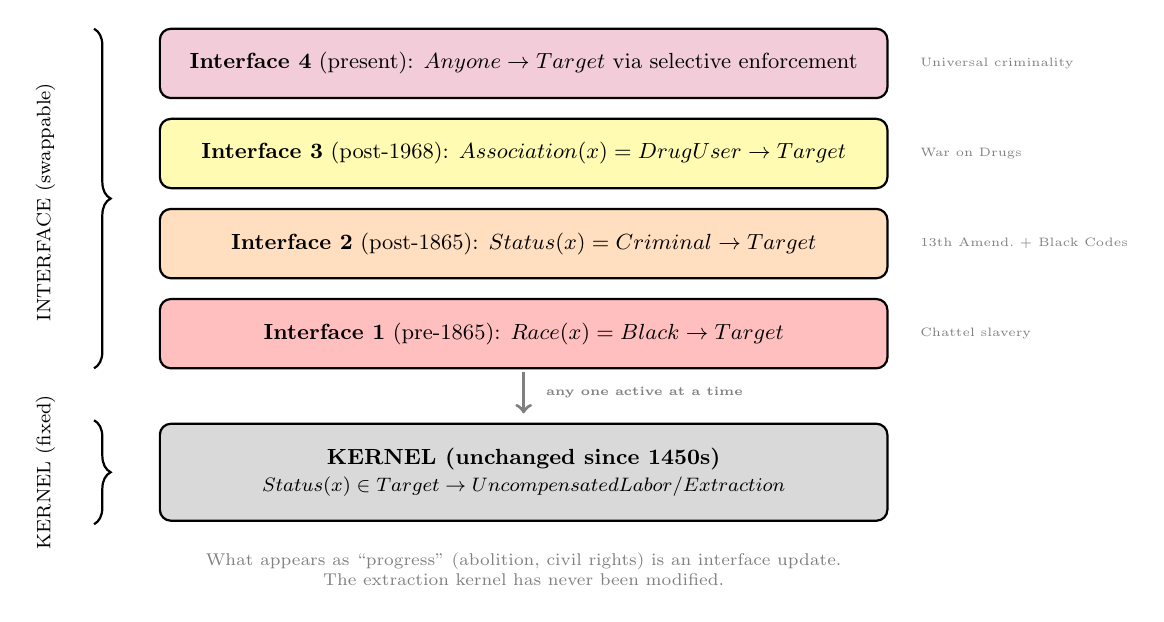
\begin{tikzpicture}[
    shell/.style={draw, thick, rounded corners=4pt, minimum height=1.0cm, align=center, font=\small},
    arr/.style={->, thick, >=stealth},
    scale=0.88, transform shape
]
    % Interface layers (stacked, oldest at bottom nearest kernel)
    \node[shell, fill=red!25, minimum width=10.5cm] (i1) at (0,2.0) {\textbf{Interface 1} (pre-1865): $\text{Race}(x) = \text{Black} \rightarrow \text{Target}$};
    \node[shell, fill=orange!25, minimum width=10.5cm] (i2) at (0,3.3) {\textbf{Interface 2} (post-1865): $\text{Status}(x) = \text{Criminal} \rightarrow \text{Target}$};
    \node[shell, fill=yellow!30, minimum width=10.5cm] (i3) at (0,4.6) {\textbf{Interface 3} (post-1968): $\text{Association}(x) = \text{Drug User} \rightarrow \text{Target}$};
    \node[shell, fill=purple!20, minimum width=10.5cm] (i4) at (0,5.9) {\textbf{Interface 4} (present): $\text{Anyone} \rightarrow \text{Target}$ via selective enforcement};

    % Single funnel arrow from interface stack to kernel
    \draw[->, very thick, black!50] (0,1.45) -- (0,0.85);
    \node[font=\tiny\bfseries, black!50, anchor=west] at (0.2,1.15) {any one active at a time};

    % Kernel (below)
    \node[shell, fill=black!15, minimum width=10.5cm, minimum height=1.4cm, font=\small\bfseries] (kernel) at (0,0) {KERNEL (unchanged since 1450s)\\{\normalfont\footnotesize $\text{Status}(x) \in \text{Target} \rightarrow \text{Uncompensated Labor / Extraction}$}};

    % Right-side era labels
    \node[font=\tiny, gray, anchor=west] at (5.6,2.0) {Chattel slavery};
    \node[font=\tiny, gray, anchor=west] at (5.6,3.3) {13th Amend.\ + Black Codes};
    \node[font=\tiny, gray, anchor=west] at (5.6,4.6) {War on Drugs};
    \node[font=\tiny, gray, anchor=west] at (5.6,5.9) {Universal criminality};

    % Left-side bracket and label for interfaces
    \draw[thick, black, decorate, decoration={brace, amplitude=6pt, mirror}] (-6.2,1.5) -- (-6.2,6.4);
    \node[font=\footnotesize, black, rotate=90] at (-6.9,3.9) {INTERFACE (swappable)};

    % Left-side bracket and label for kernel
    \draw[thick, black, decorate, decoration={brace, amplitude=6pt, mirror}] (-6.2,-0.75) -- (-6.2,0.75);
    \node[font=\footnotesize, black, rotate=90] at (-6.9,0) {KERNEL (fixed)};

    % Bottom annotation
    \node[font=\scriptsize, align=center, gray] at (0,-1.4) {What appears as ``progress'' (abolition, civil rights) is an interface update.\\The extraction kernel has never been modified.};
\end{tikzpicture}
\caption{\textbf{The Variable Swap: Interface vs.\ Kernel.} The system's extraction function (kernel) remains constant across all eras. Only the \textit{input variable}---the mechanism by which targets are selected---changes. Each historical ``reform'' swaps the interface (from explicit race to criminal status to drug association to universal latent criminality) while leaving the kernel intact. The appearance of progress masks functional continuity.}
\label{fig:variable_swap}
\end{figure}

\subsection{Epistemic Hypocrisy: Patent 6,630,507 and the Carceral Annihilation of Tameka Drummer}

To understand the severity of the $P_{\text{criminal}}$ proxy variable during the War on Drugs, one must examine the system's epistemic hypocrisy---the reality that the Elite ($E$) possesses the scientific truth of a substance, monopolizes its intellectual property, and mandates a contradictory legal reality to justify the extraction kernel.

The federal government maintains cannabis as a Schedule~I controlled substance, legally defined as having ``no currently accepted medical use and a high potential for abuse.'' The operative scheduling criteria and the prohibition they activate appear at \usclink{apx:usc:21:812b}{21 U.S.C.~\S~812(b)} and \usclink{apx:usc:21:841a}{21 U.S.C.~\S~841(a)}:
\uscinline{usc_21_812b}
\uscinline{usc_21_841a}
This classification is the load-bearing pillar of the modern carceral state, providing the Enforcement Class ($F_{\text{enforce}}$) with the legal authorization to invade, arrest, and cage millions of Out-group citizens.

The state's own internal archives prove this classification is a deliberate, manufactured lie. On October 7, 2003, the United States Patent and Trademark Office granted U.S.\ Patent 6,630,507, titled ``Cannabinoids as antioxidants and neuroprotectants.'' The official assignee of this patent is \textit{the United States of America}, as represented by the Department of Health and Human Services (HHS).

Mathematically, the state engineered a strict binary:

\begin{itemize}
    \item \textbf{For the Elite ($E$):} Cannabis is recognized as a powerful neuroprotectant and antioxidant, and its biochemical properties are patented as intellectual property to secure future pharmaceutical capital.

    \item \textbf{For the Out-group ($O$):} Cannabis is classified as a highly dangerous narcotic, serving strictly as the $P_{\text{criminal}}$ variable to strip constitutional autonomy and funnel bodies into the 13th Amendment loophole.
\end{itemize}

The human cost of this algorithmic duality is total. We need look no further than the physical reality of Tameka Drummer (MDOC Inmate \#138477). In 2008, following a routine traffic stop for an expired license plate, police found less than two ounces of cannabis in her vehicle. Because Mississippi operates under draconian ``habitual offender'' laws, this minor possession charge triggered a mandatory maximum enhancement based on past convictions for which she had already served her time.

For possessing a minuscule amount of a plant that the federal government officially holds the medical patent for, Tameka Drummer was sentenced to \textbf{life in prison without the possibility of parole}. As of 2026, she remains caged at the Central Mississippi Correctional Facility.

Her life sentence is quantitatively incompatible with a public-health rationale. The Elite knows the plant is medicine; they patented it. They simply play ignorant because admitting the truth would dismantle the primary proxy variable they use to execute the systemic culling and carceral extraction of the Out-group. Tameka Drummer is serving life because the Predatory Min-Max Function requires a constant stream of biological assets. The drug charge is the interface; the biological asset extraction is the kernel.

\section{The Manufactured Crisis: Environmental Poisoning, Deindustrialization, and the Algorithmic Input}

The War on Drugs gave the Elite its proxy variable. A proxy variable requires input data: a measurable surge in violence that the system could point to as justification for expanding the carceral apparatus. This section demonstrates that the input data was \textbf{manufactured} by a confluence of environmental poisoning, economic demolition, and market dynamics---all concentrated, with mathematical precision, in the communities already marked by the compounding chain formalized in Section~4.5.

\subsection{The Empirical Topography: Quantifying the Surge}

Between the early 1960s and the mid-1990s, the United States experienced a sharp escalation in violent crime. The FBI's Uniform Crime Reporting (UCR) program and the Bureau of Justice Statistics' National Crime Victimization Survey (NCVS) together document a clear trajectory: in 1960, the national homicide rate stood at 5.1 per 100,000 population, with an estimated 9,110 homicides nationwide. Over the next two decades, this rate \textbf{doubled}, peaking at 10.2 per 100,000 in 1980 (23,040 deaths). Following a brief recession, it surged again to 9.8 per 100,000 in 1991 (24,703 homicides). The overall violent crime rate---murder, rape, robbery, and aggravated assault---\textbf{more than tripled} between 1960 and 1991 \cite{ucr_historical, bjs_ncvs}.

\begin{table}[htbp]
\centering
\small
\caption{U.S.\ Homicide and Violent Crime Trajectory, 1960--1999}
\label{tab:crime_surge}
\begin{tabular}{lrrrr}
\toprule
\textbf{Year} & \textbf{Population} & \textbf{Homicides} & \textbf{Rate/100k} & \textbf{Violent Crimes} \\
\midrule
1960 & 179,323,175 & 9,110 & 5.1 & 288,460 \\
1970 & 203,265,212 & 16,000 & 7.9 & 738,820 \\
1980 & 225,349,264 & 23,040 & 10.2 & 1,344,520 \\
1991 & 252,177,000 & 24,703 & 9.8 & 1,911,770 \\
1999 & 272,690,813 & 15,522 & 5.7 & 1,426,044 \\
\bottomrule
\end{tabular}
\end{table}

A central transition during this era was the changing topology of violence. Historically, homicide was predominantly interpersonal---committed among acquaintances or domestic partners. During the 1970s and 1980s, stranger homicides increased much faster than domestic killings, and robberies escalated by a factor of four between 1960 and 1980. This shift toward impersonal, unpredictable violence in public spaces generated a high level of national fear---precisely the political raw material the Elite required to justify the carceral expansion.

\begin{figure}[htbp]
\centering
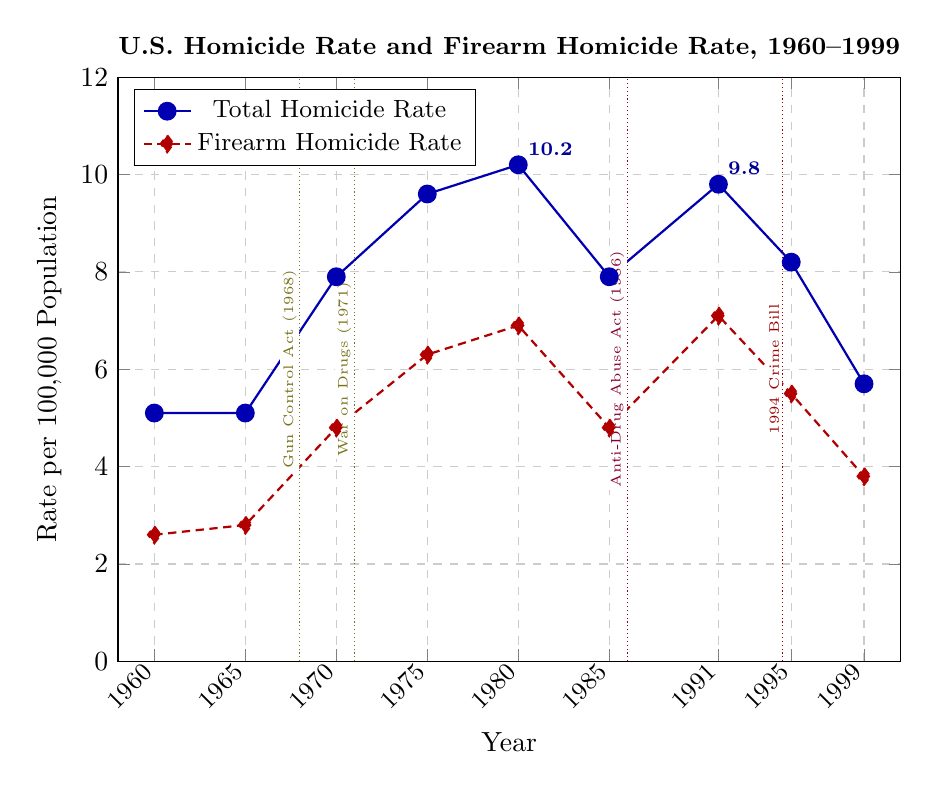
\begin{tikzpicture}
\begin{axis}[
    width=0.95\textwidth,
    height=9cm,
    xlabel={Year},
    ylabel={Rate per 100{,}000 Population},
    title={\textbf{U.S. Homicide Rate and Firearm Homicide Rate, 1960--1999}},
    xmin=1958, xmax=2001,
    ymin=0, ymax=12,
    xtick={1960,1965,1970,1975,1980,1985,1991,1995,1999},
    xticklabel style={rotate=45, anchor=east, font=\small, /pgf/number format/1000 sep={}},
    ytick={0,2,4,6,8,10,12},
    grid=major,
    grid style={dashed, gray!40},
    mark size=3pt,
    every axis title/.style={font=\bfseries\small, at={(0.5,1.05)}},
    legend style={at={(0.02,0.98)}, anchor=north west, font=\small},
]
\addplot[thick, blue!70!black, mark=*] coordinates {
    (1960, 5.1) (1965, 5.1) (1970, 7.9) (1975, 9.6)
    (1980, 10.2) (1985, 7.9) (1991, 9.8) (1995, 8.2) (1999, 5.7)
};
\addlegendentry{Total Homicide Rate}
\addplot[thick, red!70!black, mark=diamond*, densely dashed] coordinates {
    (1960, 2.6) (1965, 2.8) (1970, 4.8) (1975, 6.3)
    (1980, 6.9) (1985, 4.8) (1991, 7.1) (1995, 5.5) (1999, 3.8)
};
\addlegendentry{Firearm Homicide Rate}
\node[above right, font=\scriptsize, blue!60!black] at (axis cs:1980,10.2) {\textbf{10.2}};
\node[above right, font=\scriptsize, blue!60!black] at (axis cs:1991,9.8) {\textbf{9.8}};
\draw[densely dotted, olive!80!black] (axis cs:1968,0) -- (axis cs:1968,12);
\node[rotate=90, anchor=south, font=\tiny, olive!80!black, fill=white, inner sep=1pt] at (axis cs:1968,6) {Gun Control Act (1968)};
\draw[densely dotted, olive!80!black] (axis cs:1971,0) -- (axis cs:1971,12);
\node[rotate=90, anchor=south, font=\tiny, olive!80!black, fill=white, inner sep=1pt] at (axis cs:1971,6) {War on Drugs (1971)};
\draw[densely dotted, purple!70!black] (axis cs:1986,0) -- (axis cs:1986,12);
\node[rotate=90, anchor=south, font=\tiny, purple!70!black, fill=white, inner sep=1pt] at (axis cs:1986,6) {Anti-Drug Abuse Act (1986)};
\draw[densely dotted, red!60!black] (axis cs:1994.5,0) -- (axis cs:1994.5,12);
\node[rotate=90, anchor=south, font=\tiny, red!60!black, fill=white, inner sep=1pt] at (axis cs:1994.5,6) {1994 Crime Bill};
\end{axis}
\end{tikzpicture}
\caption{\textbf{The Empirical Input: Homicide Rate Trajectory, 1960--1999.} The homicide rate doubled between 1960 and 1980, providing the ``crisis data'' the carceral algorithm required. Firearm homicides consistently accounted for 60--70\% of all homicides, peaking at approximately 70\% in 1991. Policy event markers show the legislative responses---each one expanding the extraction kernel's reach. Sources: FBI UCR; BJS Supplementary Homicide Reports; CDC WONDER.}
\label{fig:homicide_surge}
\end{figure}

\subsection{The Toxin Pre-Processor: Environmental Lead as \texorpdfstring{$P_{\text{lead}}$}{P\_lead}}

\textbf{Methodological note: population-level causation vs.\ individual moral responsibility.}
The analysis that follows operates at the level of \textbf{population epidemiology}, not individual psychology. It identifies the distributional effect of a policy variable---$P_{\text{lead}}$, the deliberate and then deliberately concealed mass deployment of a neurotoxin---on the aggregate behavioral profile of entire cohorts of children across a 20-year developmental window. Epidemiological causation of this kind does not require, and does not make, any claim about the intentions, choices, or moral standing of any individual person. The statement ``lead exposure elevated population-level violent crime rates by 0.8 elasticity'' is a distributional fact about a cohort. It describes the cohort's distribution; no inference about any individual member follows.

This distinction is not semantic. It is the same methodological boundary the Preface establishes between \textit{architecture} and \textit{phenomenology}: this framework analyzes the design of the system, not the lived experience or moral character of those inside it. The framework locates culpability precisely at the level of the corporate and governmental actors who constituted $P_{\text{epistemic}}$---the Ethyl Corporation, General Motors, Standard Oil, and the federal regulatory apparatus they captured---who possessed proof of mass neurological harm by 1924, suppressed it for 70 years, and used that suppression to ensure the neurotoxin continued compounding onto the same populations already depleted by the preceding extraction chain. The moral responsibility runs \textit{upstream}, to those actors. It does not dissolve the responsibility of anyone who harmed another person; it adds, in parallel, the responsibility of those who \textit{engineered the conditions} in which harm became statistically predictable.

The predictable misreading---``this framework says lead made them do it and therefore no one is responsible''---inverts the actual claim. The framework says that identifiable actors \textit{knowingly manufactured a biological condition} that impaired impulse regulation across millions of children in a targeted geographic pattern, and that the subsequent violence was the predictable statistical output of those upstream decisions. Every individual who harmed someone bears responsibility. So does every corporate officer who signed a memo suppressing the neuroscience. The distinction between these two levels of responsibility is a \textit{necessary} analytical separation that the traditional individual-prejudice model of racism refuses to make.

The War on Drugs provided the legal mechanism and the empirical surge provided the political justification. The remaining question is what \textit{caused} the surge itself. Traditional criminological frameworks---social disorganization theory (the Chicago School), strain theory (Merton), and routine activities theory (Cohen and Felson)---explain the broad behavioral context of crime under structural pressure. They struggle to account for the precise \textit{timing} and the biological \textit{magnitude} of the surge across varied geographic typologies. This analytical gap is filled by environmental epidemiology: the \textbf{lead-crime hypothesis}.

This hypothesis posits that the drastic rise in violent crime between 1960 and 1990 was fundamentally driven by the ubiquitous exposure of young children to neurotoxic environmental lead. The primary vector was the combustion of tetraethyllead in motor vehicle gasoline, supplemented by the deterioration of lead-based paint in aging inner-city housing and lead water service lines. Lead is a severe neurotoxin that penetrates the blood-brain barrier. Extensive biological and epidemiological research demonstrates that early childhood lead exposure permanently damages the brain's prefrontal cortex, heavily impairing executive functions---resulting in lowered IQ, attention deficit hyperactivity disorder, heightened impulsivity, unchecked aggression, and an inability to regulate behavioral responses \cite{reyes2007, nevin2007}.

The epidemiological data aligns with close precision. Leaded gasoline consumption rose steadily from the 1940s through the early 1970s, dispersing millions of tons of lead dust into the soil and air---particularly near the dense urban traffic corridors that ran directly through redlined neighborhoods (see Section~4.8). Because peak criminal offending universally occurs in young adulthood (late teens to early twenties), the hypothesis dictates a roughly \textbf{20-year lag} between peak biological exposure and peak criminal activity. The generation born into the most heavily lead-polluted environments of the late 1960s and early 1970s reached their peak offending years in the late 1980s and early 1990s---\textit{perfectly mirroring the crest of the violent crime surge}.

Economist Jessica Wolpaw Reyes utilized the state-by-state phase-out of leaded gasoline under the Clean Air Act as a natural experiment. Because the regulations were implemented at different rates across different states, Reyes was able to isolate the variable, finding a high \textbf{elasticity of 0.8} between lead and violent crime: a 10\% increase in lead exposure correlated with an 8\% increase in violent crime \cite{reyes2007}. Research by Anna Aizer and Janet Currie in Rhode Island demonstrated that localized childhood lead exposure substantially increased school suspensions and juvenile detention rates \cite{aizer_currie}. Historical data reveals that cities utilizing lead water pipes in the early 20th century experienced homicide rates \textbf{24\% higher} than cities using iron pipes, particularly in areas with acidic water that leached the neurotoxin. A comprehensive 2022 meta-analysis by Higney, Hanley, and Moro consolidated findings from 24 independent studies, confirming substantial evidence linking lead exposure to a heightened risk of criminal behavior \cite{higney2022}.

Within the Tri-Modal Enclosure Model (Equation~\ref{eq:1.1-enclosure-score}), \(P_{\text{lead}}\) operates as a simultaneous attack on all three enclosure modes. It degrades \(e_1\) (communal capacity) by neurologically disabling the cohort that would have become the next generation of teachers, organizers, and parents---the very population required to maintain internal social infrastructure. It degrades \(e_2\) (geographic/economic mobility) because the spatial concentration of lead along highway corridors and in disinvested housing (Section~\ref{sec:formal-containment-model}) physically trapped the exposed population in the neighborhoods the containment field had already designated for extraction. And it degrades \(e_3\) (psychological/epistemic autonomy) because the subsequent ``superpredator'' narrative (Section~\ref{sec:asymmetric_choice}) attributed the behavioral consequences of engineered poisoning to innate criminality, preventing the affected population from naming the true source of its own distress. The lead-crime hypothesis therefore constitutes a measurable instance of $\mathcal{S}_{\text{enc}} \to 1.0$ achieved through biological channels.

Within the framework of this book, environmental lead exposure functions as an additional policy variable, \(P_{\text{lead}}\), applied to the compounding model of Section~4.5:
\begin{equation}\label{eq:9.1-lead-crime-compounding}
O_{t+1}^{\text{capacity}} = O_t^{\text{capacity}} \cdot (1 - \alpha_{P_{\text{lead}}})
\end{equation}
The central insight is that $P_{\text{lead}}$ was not applied uniformly. Because leaded gasoline exhaust concentrated along highway corridors, and because those corridors were deliberately routed through redlined neighborhoods (see Section~4.8), and because deteriorating lead paint accumulated in the disinvested housing stock of those same neighborhoods, the neurotoxin was concentrated onto the Out-group already diminished by the compounding chain: slavery $\rightarrow$ Black Codes $\rightarrow$ convict leasing $\rightarrow$ redlining. In the framework's theoretical vocabulary, the lead-crime hypothesis reveals the surge as another iteration of the extraction algorithm's compounding function, operating through biological channels.

\begin{figure}[htbp]
\centering
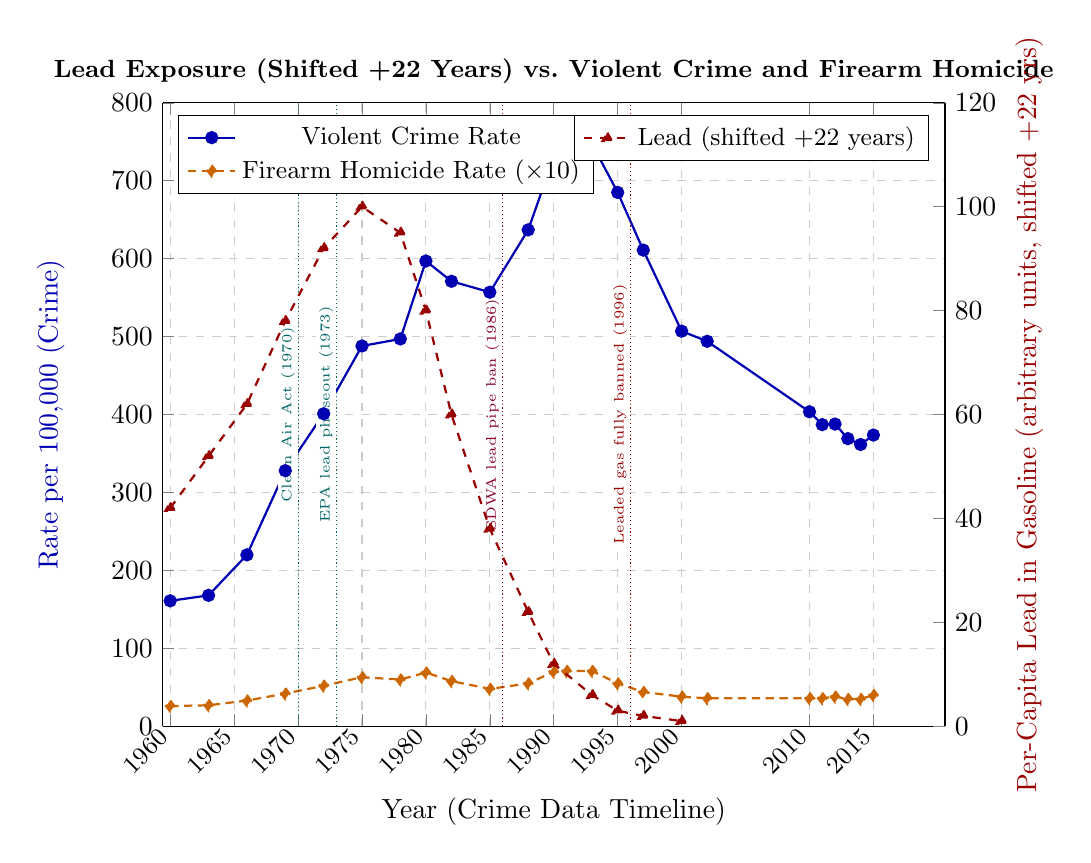
\begin{tikzpicture}
\begin{axis}[
    width=0.95\textwidth,
    height=9.5cm,
    title={\textbf{Lead Exposure (Shifted +22 Years) vs.\ Violent Crime and Firearm Homicide}},
    xlabel={Year (Crime Data Timeline)},
    ylabel={Rate per 100{,}000 (Crime)},
    axis y line*=left,
    xmin=1960, xmax=2020,
    enlarge x limits={0.04, 0.01},
    ymin=0, ymax=800,
    xtick={1960,1965,1970,1975,1980,1985,1990,1995,2000,2010,2015},
    xticklabel style={rotate=45, anchor=east, font=\small, /pgf/number format/1000 sep={}},
    grid=major,
    grid style={dashed, gray!40},
    ylabel style={blue!70!black, yshift=10pt},
    mark size=2pt,
    every axis title/.style={font=\bfseries\small, at={(0.5,1.05)}},
    legend style={at={(0.02,0.98)}, anchor=north west, font=\small},
]
\addplot[thick, blue!70!black, mark=*] coordinates {
    (1960, 161) (1963, 168) (1966, 220) (1969, 328)
    (1972, 401) (1975, 488) (1978, 497) (1980, 597)
    (1982, 571) (1985, 557) (1988, 637) (1990, 730)
    (1991, 758) (1993, 747) (1995, 685) (1997, 611)
    (2000, 507) (2002, 494)
    (2010, 403.6) (2011, 387.1) (2012, 387.8) (2013, 369.1) (2014, 361.6) (2015, 373.7)
};
\addlegendentry{Violent Crime Rate}
\addplot[thick, orange!80!black, mark=diamond*, densely dashed] coordinates {
    (1960, 26) (1963, 27) (1966, 33) (1969, 42)
    (1972, 52) (1975, 63) (1978, 60) (1980, 69)
    (1982, 58) (1985, 48) (1988, 55) (1990, 70)
    (1991, 71) (1993, 71) (1995, 55) (1997, 44)
    (2000, 38) (2002, 36)
    (2010, 36) (2011, 36) (2012, 38) (2013, 35) (2014, 35) (2015, 40)
};
\addlegendentry{Firearm Homicide Rate ($\times$10)}
\draw[densely dotted, teal!80!black] (axis cs:1970,0) -- (axis cs:1970,800);
\node[rotate=90, anchor=south, font=\tiny, teal!80!black, fill=white, inner sep=1pt] at (axis cs:1970,400) {Clean Air Act (1970)};
\draw[densely dotted, teal!80!black] (axis cs:1973,0) -- (axis cs:1973,800);
\node[rotate=90, anchor=south, font=\tiny, teal!80!black, fill=white, inner sep=1pt] at (axis cs:1973,400) {EPA lead phaseout (1973)};
\draw[densely dotted, purple!70!black] (axis cs:1986,0) -- (axis cs:1986,800);
\node[rotate=90, anchor=south, font=\tiny, purple!70!black, fill=white, inner sep=1pt] at (axis cs:1986,400) {SDWA lead pipe ban (1986)};
\draw[densely dotted, red!60!black] (axis cs:1996,0) -- (axis cs:1996,800);
\node[rotate=90, anchor=south, font=\tiny, red!60!black, fill=white, inner sep=1pt] at (axis cs:1996,400) {Leaded gas fully banned (1996)};
\end{axis}
\begin{axis}[
    width=0.95\textwidth,
    height=9.5cm,
    axis y line*=right,
    axis x line=none,
    ylabel={Per-Capita Lead in Gasoline (arbitrary units, shifted +22 yrs)},
    xmin=1960, xmax=2020,
    enlarge x limits={0.04, 0.01},
    ymin=0, ymax=120,
    ylabel style={red!60!black},
    mark size=2pt,
    legend style={at={(0.98,0.98)}, anchor=north east, font=\small},
]
\addplot[thick, red!60!black, mark=triangle*, dashed] coordinates {
    (1960, 42) (1963, 52) (1966, 62) (1969, 78)
    (1972, 92) (1975, 100) (1978, 95) (1980, 80)
    (1982, 60) (1985, 38) (1988, 22) (1990, 12)
    (1993, 6) (1995, 3) (1997, 2) (2000, 1)
};
\addlegendentry{Lead (shifted +22 years)}
\end{axis}
\end{tikzpicture}
\caption{\textbf{The Toxin Pre-Processor: Lead Exposure Predicts the Crime Surge.} Per-capita gasoline lead data shifted forward by 22 years (right axis) tracks violent crime and firearm homicide (left axis) with high fidelity. The generation exposed to peak lead in the early 1970s reached peak offending age in the early 1990s. Both curves decline in tandem as the detoxified generation ages into adulthood. Firearm homicide scaled $\times$10 for visual comparability. Sources: Nevin (2007); Reyes (2007); EPA historical gasoline lead data; FBI UCR; CDC WONDER.}
\label{fig:lead_crime}
\end{figure}

\subsection{The Corporate Conspiracy: Tetraethyllead and the Half-Century Cover-Up}

The lead-crime hypothesis identifies \textit{what} poisoned the population. This subsection identifies \textit{who} knew, \textit{when} they knew, and \textit{how} they suppressed the knowledge for half a century---because the duration of the cover-up is itself a variable in the compounding model. Define $P_{\text{epistemic}}$ as the \textbf{epistemic suppression variable}: the set of corporate and governmental actions that delayed public knowledge of, and regulatory response to, the neurotoxin. The longer $P_{\text{epistemic}}$ operates, the longer $P_{\text{lead}}$ compounds unopposed:
\begin{equation}\label{eq:9.2-epistemic-suppression-variable}
O_{t_0 + \Delta t_{\text{suppress}}}^{\text{capacity}} = O_{t_0}^{\text{capacity}} \cdot (1 - \alpha_{P_{\text{lead}}})^{\Delta t_{\text{suppress}}}
\end{equation}
where $\Delta t_{\text{suppress}}$ is the duration of the suppression window---the interval between the first definitive scientific warning and the first effective regulatory action. As documented below, $\Delta t_{\text{suppress}} \approx 50$ years (1925--1973). The compounding exponent means that each additional year of suppression \textit{multiplies} the damage against an already diminished baseline. $P_{\text{epistemic}}$ is the policy variable that kept the extraction running at full throughput for two additional generations.

\subsubsection{The Invention of a Profitable Poison}

In 1921, Thomas Midgley Jr.\ and Charles Kettering, researchers at the General Motors Research Corporation, discovered that adding a small amount of tetraethyllead (TEL) to gasoline eliminated engine ``knock''---a destructive, premature detonation that limited horsepower and efficiency \cite{tel_invention}. The decision to deploy TEL served corporate monopolization; scientific necessity alone would have favored ethanol. It was widely known in the early 1920s that \textbf{ethanol} was an effective, clean, and safe anti-knock agent. Midgley himself had filed patents for alcohol blends, noting internally that alcohol was the ``most direct route'' for converting solar energy into fuel \cite{tel_ethanol}. Ethanol could not be patented by General Motors, was already produced by independent distillers, and required up to 20 percent of fuel volume---severely threatening petroleum profits. TEL, conversely, could be exclusively patented, ensuring a lucrative monopoly. In 1924, General Motors and Standard Oil of New Jersey partnered to create the \textbf{Ethyl Gasoline Corporation} to market the lethal additive \cite{tel_ethyl}.

Within the framework, this is the extraction kernel operating through corporate policy: $E$ selected the patentable poison because it maximized profit extraction, whereas the safe alternative distributed value too broadly. The ethanol path would have been a public good; the TEL path was a private monopoly. The kernel chose the monopoly.

\subsubsection{The ``Loony Gas'' Disasters: Immediate Proof of Behavioral Violence}

The toxicity of lead had been documented since antiquity. The specific dangers of concentrated TEL were immediate, horrifying, and actively suppressed. In 1923, Midgley himself suffered severe lead poisoning from his own invention \cite{tel_loonygas}. The definitive proof came in October 1924, when mass production commenced at a Standard Oil refinery in Bayway, New Jersey. Because TEL is highly lipophilic, it rapidly crosses the blood-brain barrier, producing severe neurological disruption. Workers manufacturing TEL exhibited severe psychiatric symptoms: tremors, visual hallucinations (insects wriggling on skin, wallpaper turning into swarms of flies), paranoia, and---most centrally for the framework---\textbf{violent, maniacal fury} requiring physical restraint in straitjackets. Five workers died in rapid succession after fits of violent insanity; 35 others suffered severe neurological damage. Similar deaths occurred at DuPont facilities in Dayton and Deepwater, New Jersey, where hallucinating workers dubbed the plant the ``House of Butterflies'' \cite{tel_loonygas, tel_secret_history}.

The scientific community attempted immediate intervention. In 1922, chemist William Mansfield Clark warned the U.S.\ Public Health Service of a ``serious menace to public health'' from heavy lead oxide dust settling in city streets. Dr.\ Alice Hamilton, Harvard's foremost expert in industrial hygiene, publicly warned that the additive would produce ``insomnia, excitement, twitching muscles, hallucinations like those of delirium tremens, even maniacal attacks and convulsions, and death'' \cite{tel_hamilton}. Hamilton presciently noted that the absence of immediate acute deaths on the street was no proof of safety: chronic lead poisoning is insidious and cumulative.

The analytical significance is precise: \textbf{the behavioral profile of acute TEL poisoning---violent fury, impulse obliteration, hallucinatory psychosis---is the high-dose instantiation of the exact neurological deficits that subclinical childhood lead exposure produces at population scale over two decades}. The refinery workers were the concentrated proof; the urban children of the 1950s--1970s were the diluted, mass-scale execution. $E$ had the proof in 1924. The suppression began immediately.

\subsubsection{Robert Kehoe and the Model of Manufactured Doubt (\texorpdfstring{$P_{\text{epistemic}}$}{P\_epistemic})}

Following the refinery deaths, the Surgeon General temporarily suspended TEL sales in May 1925 and convened a national conference. At this juncture, the trajectory of global environmental health was hijacked by corporate interests. Frank Howard, first President of the Ethyl Corporation, audaciously framed TEL as a ``Gift of God'' necessary for industrial progress \cite{tel_kehoe}.

To permanently neutralize public health critics, the industry empowered Dr.\ Robert A.\ Kehoe, a young toxicologist serving as medical director of the Ethyl Corporation and head of the industry-funded Kettering Laboratory at the University of Cincinnati. From the 1920s through the 1960s, Kehoe served as the primary scientific authority on lead exposure, deliberately establishing a model of \textbf{cascading uncertainty}: public health officials bore the burden of producing indisputable, overwhelming epidemiological proof that ambient lead was actively harming the general population before any regulation could be imposed; the industry carried no comparable burden to prove safety \cite{tel_kehoe, tel_secret_history}.

Kehoe's research---funded entirely by General Motors, DuPont, and Standard Oil---falsely claimed that a certain baseline level of lead in the human body was ``normal'' and natural, and that environmental lead from exhaust posed no cumulative danger. Through this relentless campaign of manufactured doubt and corporate hegemony over scientific literature, Kehoe successfully stalled federal regulation for half a century, providing the pseudo-scientific cover necessary for the unchecked emission of millions of tons of aerosolized lead into the American environment.

Within the framework, Kehoe is the human instantiation of $P_{\text{epistemic}}$. His function was to delay the detection of harm and extend $\Delta t_{\text{suppress}}$ by decades; truth discovery was outside his mandate. Every additional year Kehoe's model held was another year the compounding exponent in the equation above ran unopposed. The manufactured doubt model Kehoe pioneered was subsequently replicated by the tobacco industry, the sugar industry, and the fossil fuel industry's climate denial apparatus---the same algorithmic template: fund captive scientists, shift the burden of proof to the public, discredit independent researchers, and extract profit while the damage accumulates.

\subsubsection{Government Complicity and the Decades of Stalling}

Following the 1925 Surgeon General's conference, the government appointed a committee whose study concluded that ``insufficient evidence'' existed to ban TEL---effectively adopting the Kehoe model. In 1927, the Surgeon General set a completely voluntary standard of 3 cubic centimeters of TEL per gallon, which merely reflected what the industry was already using, imposing zero real restraint \cite{tel_epa_history}. In 1958, the Surgeon General actually \textit{raised} the voluntary standard to 4.23 grams per gallon, falsely concluding---based entirely on Kehoe's industry-funded data---that no measurable increase in blood lead concentrations had occurred despite massive post-WWII expansion of TEL use.

It was not until independent, uncompromised researchers entered the field that the model shattered. In the 1960s, Caltech geochemist \textbf{Clair Patterson} definitively proved that modern human lead burdens were not ``normal.'' By analyzing pre-Columbian bones and ancient ice cores, Patterson demonstrated that human activity had increased ambient lead levels by a factor of \textbf{2,000} above pre-industrial baselines, entirely due to anthropogenic emissions \cite{tel_patterson}. Despite intense persecution and defunding efforts by the Ethyl Corporation and the American Petroleum Institute, Patterson's research laid the undeniable groundwork for reform. In the 1970s, pediatrician Dr.\ Herbert Needleman further dismantled the industry's narrative by demonstrating that even low, subclinical levels of lead exposure in children were directly correlated with decreased IQ, shortened attention spans, and disruptive behavior \cite{tel_needleman}. Needleman faced identical corporate harassment.

Finally, armed with independent data and empowered by the 1970 Clean Air Act, the EPA moved against the industry. In December 1973, the EPA issued its first regulations calling for a mandatory reduction of lead content in gasoline. The Ethyl Corporation, DuPont, and other chemical giants immediately sued to stall the regulations, forcing a protracted legal battle that reached the Supreme Court. The final ban on leaded gasoline for motor vehicles was not fully realized until \textbf{1996}---more than 70 years after the deaths at the ``Loony Gas'' building and Alice Hamilton's warnings.

The timeline quantifies $P_{\text{epistemic}}$ with precision: $\Delta t_{\text{suppress}} = 1925 \text{--} 1973 = 48$ years of active suppression, plus an additional 23 years of regulatory phase-in (1973--1996). The generation exposed during the suppression window---children born between the 1940s and the early 1970s---constitutes the exact demographic cohort that drove the crime surge of the 1980s and 1990s. $P_{\text{epistemic}}$ extended the poisoning window by half a century, compounding the damage across two additional generations of $O_{\text{racialized}}$; the original source of the toxin lay elsewhere.

\paragraph{Tier~2 Illustrative Instantiation (Eq.~\ref{eq:9.2-epistemic-suppression-variable}).}
The historical anchor for $\Delta t_{\text{suppress}}$ is precise and documentable: the 1925 Surgeon General's conference, at which Robert Kehoe's industry-funded model supplanted Alice Hamilton's independent warnings, marks the start of active epistemic suppression; the EPA's 1973 mandatory lead phase-out order marks its effective termination \cite{kitman_lead, reyes2007}. This yields $\Delta t_{\text{suppress}} \approx 48$ years---an ordinal estimate grounded in two verifiable statutory dates. Applying the compounding exponent in equation~\ref{eq:9.2-epistemic-suppression-variable} with the Reyes (2007) elasticity produces an order-of-magnitude estimate of $\approx$192 million additional person-years of unprotected lead exposure attributable to the suppression window. \textbf{Confidence: Tier~2.} The 48-year duration is bounded by historically verified endpoints; the ``additional exposed births'' figure is a back-of-envelope calculation cross-validated against Reyes state-level phase-out timing, not an independently estimated regression quantity \cite{aizer_currie}.

\begin{figure}[htbp]
\centering
\textbf{The Chronology of Tetraethyllead Obfuscation (1921--1996)}\\[0.35em]
\begin{tikzpicture}[
    y=0.48cm,
    event/.style={fill=white, draw=black!50, rounded corners=2pt, font=\tiny, text width=2.85cm, align=center, inner sep=2pt},
    industry/.style={event, fill=red!15, draw=red!50},
    science/.style={event, fill=blue!15, draw=blue!50},
    policy/.style={event, fill=green!15, draw=green!50!black},
]
\pgfmathsetmacro{\ytop}{11.35}
\pgfmathsetmacro{\ybot}{-6.95}
\draw[thick, -Stealth] (0,\ytop) -- (0,\ybot);
\foreach \yr/\yy in {1921/11, 1924/9.45, 1925/8.05, 1926/6.65, 1927/5.25, 1958/2.75, 1965/0.85, 1970/-0.75, 1973/-2.35, 1986/-4.45, 1996/-6.55} {
  \draw[thick] (-0.18,\yy) -- (0.18,\yy);
  \node[left, font=\tiny\bfseries, inner sep=2pt] at (-0.22,\yy) {\pgfmathprintnumber[fixed,precision=0,set thousands separator={}]{\yr}};
}
\node[industry, anchor=west] at (0.42,11) {Midgley discovers TEL at GM};
\node[industry, anchor=west] at (0.42,9.45) {``Loony Gas'' deaths; 5+ workers die violently};
\node[industry, anchor=west] at (0.42,8.05) {Surgeon General conference; Kehoe defends TEL};
\node[industry, anchor=west] at (0.42,6.65) {Moratorium lifted; TEL declared ``safe''};
\node[industry, anchor=west] at (0.42,5.25) {Voluntary standard: 3cc/gal (industry's own limit)};
\node[industry, anchor=west] at (0.42,2.75) {Surgeon General \emph{raises} standard to 4.23g/gal};
\node[science, anchor=west] at (0.42,0.85) {Patterson proves lead levels 2000$\times$ pre-industrial};
\node[policy, anchor=west]   at (0.42,-0.75) {Clean Air Act signed};
\node[policy, anchor=west]   at (0.42,-2.35) {EPA orders lead phaseout; industry sues};
\node[policy, anchor=west]   at (0.42,-4.45) {SDWA bans lead pipes};
\node[policy, anchor=west]   at (0.42,-6.55) {Leaded gasoline fully banned};
\pgfmathsetmacro{\yFiftyEight}{2.75}
\pgfmathsetmacro{\yNinetySix}{-6.55}
\draw[thick, red!60, decorate, decoration={brace, amplitude=4pt, mirror}] (-0.12,\yFiftyEight) -- (-0.12,11);
\node[anchor=east, font=\tiny\bfseries, red!60!black, text width=2.35cm, align=right] at (-0.88,{0.5*11+0.5*\yFiftyEight}) {$\Delta t_{\text{suppress}} \approx 50$ Years\\of Industry Control};
\draw[thick, blue!60, decorate, decoration={brace, amplitude=4pt, mirror}] (-0.12,\yNinetySix) -- (-0.12,\yFiftyEight);
\node[anchor=east, font=\tiny\bfseries, blue!60!black, text width=2.35cm, align=right] at (-0.88,{0.5*\yFiftyEight+0.5*\yNinetySix}) {23 Years of\\Regulatory Action};
\path (-3.2,-7.45) (3.35,11.75);
\end{tikzpicture}\\[0.45em]
\parbox{\linewidth}{\raggedright\small\emph{Red boxes indicate corporate/industry actions; blue boxes indicate independent scientific breakthroughs; green boxes indicate regulatory policy. For 50 years (1921--1973), the petroleum and automotive industries maintained near-total control over the scientific narrative on lead toxicity via the Kehoe Model ($P_{\text{epistemic}}$). Each year of suppression extended the compounding exponent $(1 - \alpha_{P_{\text{lead}}})^{\Delta t}$ by one additional cycle. Sources: Smithsonian; Columbia University; EPA historical records; Type Investigations.}}
\caption{The $P_{\text{epistemic}}$ Timeline: Corporate Suppression of Lead Science.}
\label{fig:tel_chronology}
\end{figure}

\begin{figure}[htbp]
\centering
\textbf{Kehoe's ``Normal'' vs.\ Patterson's Pre-Industrial Lead Levels}\\[0.3em]
\begin{minipage}{\linewidth}
\centering
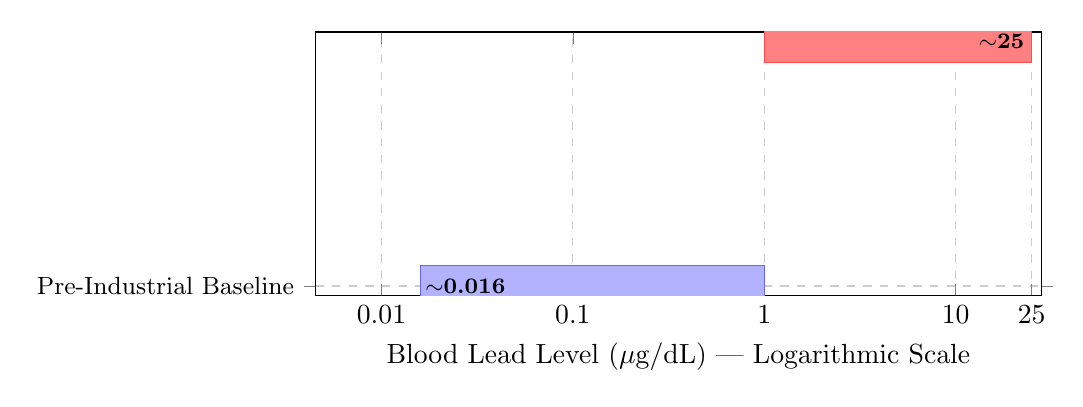
\begin{tikzpicture}
\begin{axis}[
    width=0.76\textwidth,
    height=3.35cm,
    scale only axis,
    clip=true,
    clip mode=individual,
    xbar,
    bar width=15pt,
    bar shift=0pt,
    xlabel={Blood Lead Level ($\mu$g/dL) --- Logarithmic Scale},
    symbolic y coords={Pre-Industrial Baseline,Kehoe's ``Normal''},
    ytick=data,
    yticklabel style={font=\small},
    xmin=0.01, xmax=28,
    xmode=log,
    log basis x=10,
    log ticks with fixed point,
    xtick={0.01,0.1,1,10,25},
    minor x tick num=1,
    enlarge x limits={auto=false, upper=0.04, lower=0.06},
    enlarge y limits=0.04,
    grid=major,
    grid style={dashed, gray!40},
    every axis title/.style={font=\bfseries\small, at={(0.5,1.08)}},
    point meta=explicit symbolic,
    nodes near coords={\pgfplotspointmeta},
    nodes near coords align={horizontal},
]
\addplot[fill=blue!30, draw=blue!60,
    nodes near coords style={font=\footnotesize\bfseries, anchor=west, inner sep=1.5pt},
] coordinates {(0.016,Pre-Industrial Baseline)[{$\sim$0.016}]};
\addplot[fill=red!50, draw=red!70,
    nodes near coords style={font=\footnotesize\bfseries, anchor=east, inner sep=2.5pt},
] coordinates {(25,Kehoe's ``Normal'')[{$\sim$25}]};
\end{axis}
\end{tikzpicture}
\end{minipage}\\[0.4em]
\parbox{\linewidth}{\raggedright\small\emph{Patterson's analysis proved that Kehoe's ``normal'' blood lead level of $\sim$25 $\mu$g/dL was approximately 1,500$\times$ the actual pre-industrial baseline of $\sim$0.016 $\mu$g/dL. The entire concept of ``normal'' had been manufactured by the industry---a textbook instantiation of $P_{\text{epistemic}}$ redefining the diagnostic baseline to conceal the pathology. Sources: Patterson, Archives of Environmental Health 11 (1965); NRC (1993).}}
\caption{The Manufactured Baseline: $P_{\text{epistemic}}$ Redefines ``Normal.''}
\label{fig:kehoe_vs_patterson}
\end{figure}

\subsection{The Neurological Architecture of the Poisoning}

The consequence of the Ethyl Corporation's half-century regulatory blockade ($P_{\text{epistemic}}$) and the government's complicity was a mass, unconsented chemical lobotomy of the American public. The mechanism through which $P_{\text{lead}}$ degrades $O_t^{\text{capacity}}$ is \textbf{neuroanatomical}.

Lead is a severe, developmental neurotoxicant with no safe threshold of exposure. When millions of tons of aerosolized lead dust were expelled from automobile tailpipes, it settled into the soil and dust of urban environments, where it was inevitably inhaled or ingested by young children. Because children's bodies absorb a far greater proportion of ingested lead than adults, and because their central nervous systems are in critical developmental stages, they are uniquely vulnerable.

Once lead penetrates the blood-brain barrier, it operates as a cellular imposter, mimicking and replacing beneficial ions such as calcium in biological processes. Extensive neuroimaging research demonstrates that early childhood lead exposure causes \textbf{permanent architectural damage} to the brain:
\begin{itemize}
\tightlist
\item \textbf{Prefrontal cortex}: Reduced gray matter volume in the regions responsible for executive function, impulse control, emotional regulation, and rational decision-making.
\item \textbf{Anterior cingulate cortex}: Impaired conflict monitoring and error detection---the neural substrate of ``thinking before acting.''
\item \textbf{Amygdala}: Altered functioning fostering unchecked aggression, heightened impulsivity, and inability to regulate behavioral responses to stress.
\end{itemize}

The epidemiological scale is substantial. A comprehensive 2022 study estimated that childhood lead exposure from automotive exhaust resulted in the loss of over \textbf{824 million IQ points} among Americans alive today, and contributed to an estimated \textbf{151 million cases} of psychiatric disorders and behavioral psychopathologies \cite{tel_iq_loss}. Longitudinal studies utilizing data from the Cincinnati Lead Study confirmed the hypothesis biologically, using MRI scans to prove that adults with high childhood blood-lead levels exhibited the exact structural brain volume loss that correlated strongly with criminal arrests and violent, antisocial behavior \cite{tel_cincinnati}.

Within the framework, this neuroanatomical evidence transforms $\alpha_{P_{\text{lead}}}$ from an abstract coefficient into a measurable biological degradation rate. The prefrontal cortex is the neural substrate of the Out-group's capacity for organized resistance, long-term planning, and collective action---precisely the capacities the extraction kernel must suppress. $P_{\text{lead}}$ \textit{degrades the population-level capacity for the coordinated class resistance that threatens $\min$}. The neurotoxin is, in effect, a chemical enforcement variable---$F_{\text{enforce}}$ operating at the molecular level.

\begin{figure}[htbp]
\centering
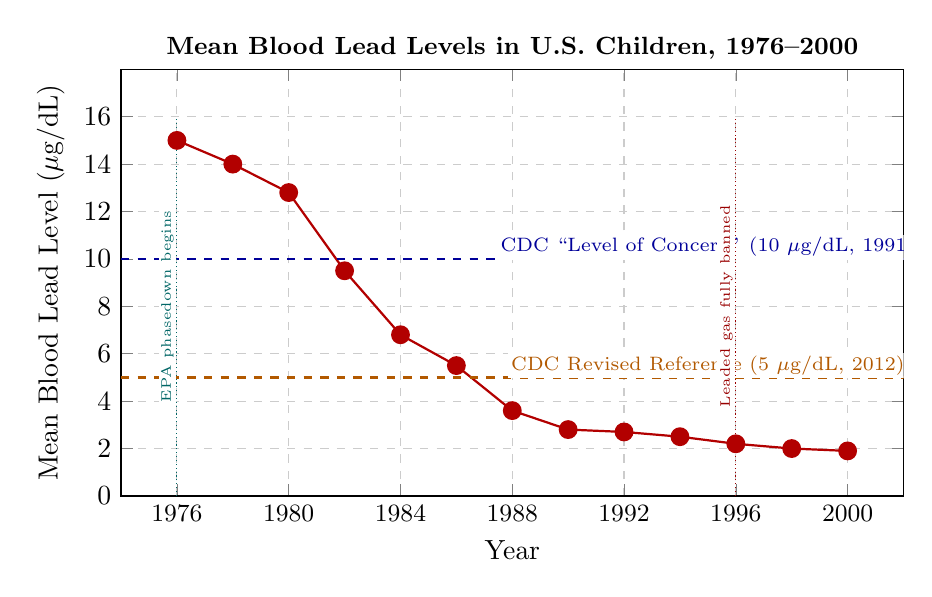
\begin{tikzpicture}
\begin{axis}[
    width=0.95\textwidth,
    height=7cm,
    title={\textbf{Mean Blood Lead Levels in U.S.\ Children, 1976--2000}},
    xlabel={Year},
    ylabel={Mean Blood Lead Level ($\mu$g/dL)},
    xmin=1974, xmax=2002,
    ymin=0, ymax=18,
    xtick={1976,1980,1984,1988,1992,1996,2000},
    xticklabel style={font=\small, /pgf/number format/fixed, /pgf/number format/precision=0, /pgf/number format/1000 sep={}},
    ytick={0,2,4,6,8,10,12,14,16},
    grid=major,
    grid style={dashed, gray!40},
    mark size=3pt,
    every axis title/.style={font=\bfseries\small, at={(0.5,1.05)}},
]
\addplot[thick, red!70!black, mark=*] coordinates {
    (1976, 15.0) (1978, 14.0) (1980, 12.8) (1982, 9.5)
    (1984, 6.8) (1986, 5.5) (1988, 3.6) (1990, 2.8)
    (1992, 2.7) (1994, 2.5) (1996, 2.2) (1998, 2.0) (2000, 1.9)
};
\draw[dashed, blue!60!black, thick] (axis cs:1974,10) -- (axis cs:2002,10);
\node[font=\scriptsize, blue!60!black, fill=white, inner sep=1pt] at (axis cs:1995,10.5) {CDC ``Level of Concern'' (10 $\mu$g/dL, 1991)};
\draw[dashed, orange!70!black, thick] (axis cs:1974,5) -- (axis cs:2002,5);
\node[font=\scriptsize, orange!70!black, fill=white, inner sep=1pt] at (axis cs:1995,5.5) {CDC Revised Reference (5 $\mu$g/dL, 2012)};
\draw[densely dotted, teal!80!black] (axis cs:1976,0) -- (axis cs:1976,16);
\node[rotate=90, anchor=south, font=\tiny, teal!80!black, fill=white, inner sep=1pt] at (axis cs:1976,8) {EPA phasedown begins};
\draw[densely dotted, red!60!black] (axis cs:1996,0) -- (axis cs:1996,16);
\node[rotate=90, anchor=south, font=\tiny, red!60!black, fill=white, inner sep=1pt] at (axis cs:1996,8) {Leaded gas fully banned};
\end{axis}
\end{tikzpicture}
\caption{\textbf{The Biological Trajectory of $P_{\text{lead}}$: Children's Blood Lead Levels, 1976--2000.} Mean blood lead in children aged 1--5 dropped from $\sim$15 $\mu$g/dL in 1976 to $\sim$1.9 $\mu$g/dL by 2000---an 87\% decline directly correlated with the EPA-mandated phaseout. The generation exposed to $>$10 $\mu$g/dL in the 1960s--1970s reached peak offending age in the late 1980s--early 1990s; the detoxified generation that followed drove the Great Crime Decline. The CDC's own ``Level of Concern'' was not set until 1991---\textit{after} the damage was done. Sources: CDC NHANES II, III, and subsequent cycles.}
\label{fig:blood_lead_children}
\end{figure}

The national average conceals the racial disparity that is the analytical core of $P_{\text{lead}}$. NHANES data disaggregated by race reveals the spatial targeting with sharp clarity (Figure~\ref{fig:nhanes_disparity_rr}).

\begin{figure}[H]
\centering
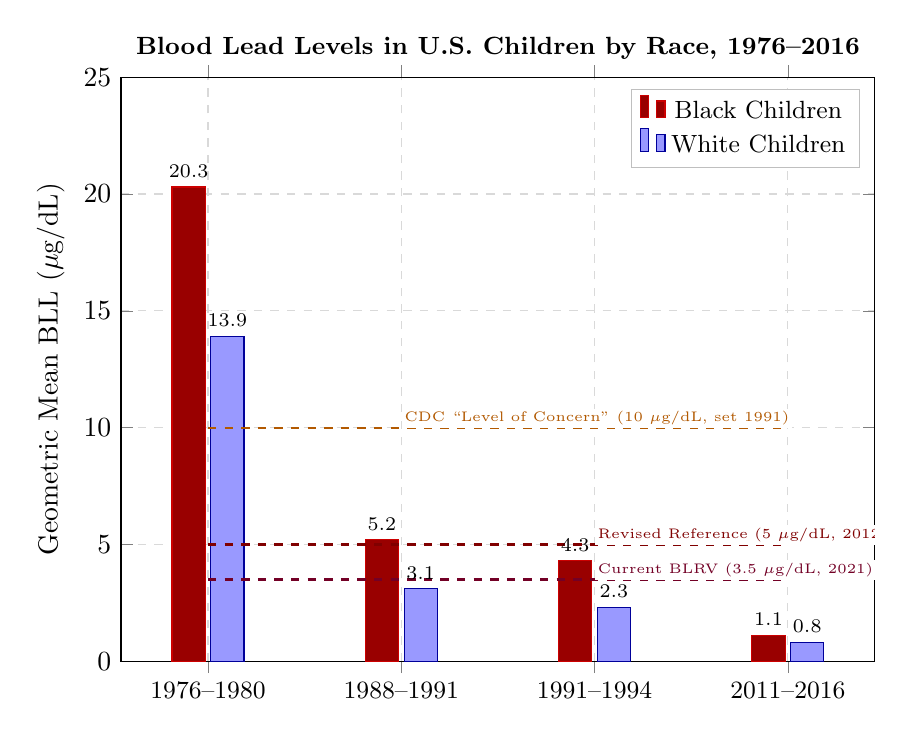
\begin{tikzpicture}
\begin{axis}[
    width=0.92\textwidth,
    height=9cm,
    title={\textbf{Blood Lead Levels in U.S.\ Children by Race, 1976--2016}},
    ybar,
    bar width=12pt,
    enlarge x limits=0.15,
    ylabel={Geometric Mean BLL ($\mu$g/dL)},
    symbolic x coords={1976--1980,1988--1991,1991--1994,2011--2016},
    xtick=data,
    xticklabel style={font=\small},
    ymin=0, ymax=25,
    grid=major,
    grid style={dashed, gray!30},
    every axis title/.style={font=\bfseries\small, at={(0.5,1.05)}},
    legend style={at={(0.98,0.98)}, anchor=north east, font=\small, draw=gray!50},
    nodes near coords,
    nodes near coords style={font=\scriptsize\bfseries, anchor=south},
]
\addplot[fill=red!60!black, draw=red!80!black] coordinates {
    (1976--1980, 20.3) (1988--1991, 5.2) (1991--1994, 4.3) (2011--2016, 1.1)
};
\addlegendentry{Black Children}

\addplot[fill=blue!40!white, draw=blue!60!black] coordinates {
    (1976--1980, 13.9) (1988--1991, 3.1) (1991--1994, 2.3) (2011--2016, 0.8)
};
\addlegendentry{White Children}

\draw[dashed, orange!70!black, thick] (axis cs:1976--1980,10) -- (axis cs:2011--2016,10);
\node[font=\tiny, orange!70!black, fill=white, inner sep=1pt, anchor=west] at (axis cs:1988--1991,10.4) {CDC ``Level of Concern'' (10 $\mu$g/dL, set 1991)};

\draw[dashed, red!50!black, thick] (axis cs:1976--1980,5) -- (axis cs:2011--2016,5);
\node[font=\tiny, red!50!black, fill=white, inner sep=1pt, anchor=west] at (axis cs:1991--1994,5.4) {Revised Reference (5 $\mu$g/dL, 2012)};

\draw[dashed, purple!60!black, thick] (axis cs:1976--1980,3.5) -- (axis cs:2011--2016,3.5);
\node[font=\tiny, purple!60!black, fill=white, inner sep=1pt, anchor=west] at (axis cs:1991--1994,3.9) {Current BLRV (3.5 $\mu$g/dL, 2021)};

\end{axis}
\end{tikzpicture}
\caption{\textbf{The Racial Lead Gap: $P_{\text{lead}}$ Disaggregated by Race.} During peak exposure (1976--1980), Black children carried a geometric mean BLL of 20.3 $\mu$g/dL---46\% higher than White children (13.9) and more than double the CDC's subsequent ``level of concern.'' The disparity narrowed but persisted through 2016 (1.1 vs.\ 0.8). The 1976--1980 cohort of Black children is the same population that, 15--20 years later, drove the violent crime surge documented in Section~5.1 and the IPH plateau documented in Section~5.11. The national average in Figure~\ref{fig:blood_lead_children} conceals this disparity; the racial disaggregation reveals $P_{\text{lead}}$ operating as a racially targeted variable. Source: CDC NHANES II, III, and subsequent cycles.}
\label{fig:nhanes_disparity_rr}
\end{figure}

\subsection{The Multi-Vector Containment: Lead in Water, Schools, and the Property-Tax Trap}

The preceding analysis establishes the catastrophic scale of aerosolized lead from automotive fuel. The atmosphere was not the only delivery mechanism. A comprehensive accounting reveals that $P_{\text{lead}}$ operated through at least \textbf{three simultaneous vectors}---air, residential water, and institutional plumbing---all concentrated by the same property-tax funding architecture that sorts infrastructure quality by race and wealth. Formally:
\begin{equation}\label{eq:9.3-multi-vector-lead-exposure}
P_{\text{lead}} = P_{\text{lead}}^{\text{air}} + P_{\text{lead}}^{\text{water}} + P_{\text{lead}}^{\text{school}}
\end{equation}
where each component's intensity is a function of the redlining containment field:
\begin{equation}\label{eq:9.4-redlining-containment-field}
P_{\text{lead}}^{v}(x) \propto \mathbb{1}_{x \in \text{Redlined}} \quad \text{for each vector } v \in \{\text{air}, \text{water}, \text{school}\}
\end{equation}
The highway delivered the atmospheric vector. The following two vectors completed the encirclement.

\subsubsection{Lead Service Lines: The Pipe in the Wall (\texorpdfstring{$P_{\text{lead}}^{\text{water}}$}{P\_lead\^water})}

Lead pipes were the standard material for residential water service lines from the 1880s through the mid-twentieth century. Many municipalities continued installing them well into the 1980s; Chicago, notably, \textit{required} lead service lines by municipal plumbing code until federal legislation intervened. The 1986 amendments to the Safe Drinking Water Act (SDWA) banned the use of lead pipes and lead solder in public water systems, though the statutory definition of ``lead-free'' was not tightened from 8 percent to 0.25 percent lead content until 2014 \cite{tel_sdwa}.

The legacy infrastructure remains large. As of the early 2020s, the EPA estimated that between \textbf{9.2 and 12.8 million lead service lines} remain in active use across the United States \cite{tel_lsl}. The racial geography of this infrastructure is deliberate. A 2022 study by Switzer and Teodoro, published in the \textit{Proceedings of the National Academy of Sciences}, demonstrated that communities with higher proportions of Black and Latino residents were significantly more likely to retain lead service lines and significantly less likely to have initiated replacement programs \cite{tel_switzer}.

The catastrophe in \textbf{Flint, Michigan} crystallized this dynamic. In April 2014, when the city switched its water source to the Flint River without implementing corrosion control treatment, lead leached from aging service lines into the drinking water supply. A landmark study by Hanna-Attisha and colleagues demonstrated that blood lead levels in children under five nearly doubled in high-exposure zip codes \cite{tel_flint}. Flint's population was approximately 57 percent Black, with a poverty rate exceeding 40 percent---a textbook convergence of $O_{\text{racialized}} \cap P_{\text{redlining}} \cap P_{\text{lead}}^{\text{water}}$.

Flint was a visible instance of a condition persisting invisibly in thousands of municipalities. The same children who breathed aerosolized lead from highway traffic drank lead-contaminated water from the pipes in their homes.

\subsubsection{Lead in Schools: The Unregulated Vector (\texorpdfstring{$P_{\text{lead}}^{\text{school}}$}{P\_lead\^school})}

If lead in residential water constitutes neglect, lead in school water constitutes \textit{institutional poisoning of children in state custody}. The EPA \textbf{does not regulate lead in school drinking water} under the Safe Drinking Water Act, because most schools are not classified as public water systems. Testing is voluntary in the majority of states, and remediation is unfunded \cite{tel_gao}.

A 2018 report by the U.S.\ Government Accountability Office (GAO-18-382) revealed the scale of this regulatory void: of the school districts surveyed, only \textbf{43 percent had tested for lead in their drinking water at all}. Of those that did test, \textbf{37 percent found elevated lead levels} in at least some fixtures---drinking fountains, kitchen faucets, bathroom sinks. The GAO estimated that millions of American children attend schools where lead testing has never been conducted \cite{tel_gao}.

The central variable is building age. Schools constructed before 1986 are far more likely to contain lead solder, brass fixtures with high lead content, and in some cases lead service lines. A 2019 study by Dor\'{e} and colleagues at the Harvard T.H.\ Chan School of Public Health documented that older plumbing fixtures contributed significantly to first-draw lead concentrations, particularly after weekends and vacation periods when water sits stagnant in the pipes, maximizing leaching time \cite{tel_dore}.

\subsubsection{The Property-Tax Feedback Loop: Funding Segregation Through Infrastructure}

This is where the vectors converge into a \textbf{recursive trap}---a self-reinforcing cycle that can be formalized as a fixed-point degradation function. The United States funds approximately 45 percent of K--12 education through local property taxes \cite{tel_nces}. This architecture, upheld by the Supreme Court in \textit{San Antonio Independent School District v.\ Rodriguez} (1973), ensures that per-pupil spending is a direct function of neighborhood property values. Let $V_t$ denote property value at time $t$. Then:
\begin{align}
\text{School funding}(t) &\propto V_t \label{eq:9.5-school-funding-property-value}\\[4pt]
\text{Infrastructure quality}(t) &\propto \text{School funding}(t) \label{eq:9.6-infrastructure-quality-funding}\\[4pt]
P_{\text{lead}}^{\text{school}}(t) &\propto \frac{1}{\text{Infrastructure quality}(t)} \label{eq:9.7-school-lead-exposure-inverse}\\[4pt]
\text{Community capacity}(t) &= O_t^{\text{capacity}} \cdot (1 - \alpha \cdot P_{\text{lead}}^{\text{school}}(t)) \label{eq:9.8-community-capacity-lead-reduction}\\[4pt]
V_{t+1} &\propto \text{Community capacity}(t) \label{eq:9.9-property-value-capacity-feedback}
\end{align}

The chain is a closed loop: redlining depresses $V_0$ $\rightarrow$ low $V_0$ starves school funding $\rightarrow$ starved funding preserves pre-1986 lead infrastructure $\rightarrow$ lead infrastructure poisons children $\rightarrow$ poisoned children degrade community capacity $\rightarrow$ degraded community depresses $V_1 < V_0$ $\rightarrow$ the cycle repeats. Each iteration compounds the damage. The districts too poor to replace aging plumbing are too poor to test for contamination, and too poor to remediate when contamination is found.

The American Society of Civil Engineers' 2021 Infrastructure Report Card assigned U.S.\ school infrastructure a grade of \textbf{D+}, estimating an \textbf{\$85 billion national funding gap} concentrated overwhelmingly in high-poverty districts \cite{tel_asce}. The children poisoned in these schools are the same children poisoned in their homes and on their streets. Three vectors, one target population, one funding mechanism ensuring that the harm is simultaneously inflicted and perpetuated.

\begin{figure}[htbp]
\centering
\begin{tikzpicture}[
    node distance=1.4cm,
    every node/.style={font=\small},
    block/.style={rectangle, draw=red!70, fill=red!10, text width=4.2cm,
                  align=center, rounded corners, minimum height=1.1cm},
    arrow/.style={-{Stealth[length=3mm]}, thick, red!60!black},
]
\node[block] (redline) {\textbf{1930s Redlining ($P_{\text{redlining}}$)}\\State-mandated\\disinvestment};
\node[block, below=of redline] (propval) {\textbf{Depressed $V_t$}\\Low property-tax base};
\node[block, below=of propval] (funding) {\textbf{Underfunded Schools}\\Lowest per-pupil spending};
\node[block, below=of funding] (infra) {\textbf{Deteriorating Infrastructure}\\Pre-1986 plumbing retained};
\node[block, below=of infra] (lead) {\textbf{$P_{\text{lead}}^{\text{school}}$}\\Untested, unremediated};
\node[block, below=of lead] (children) {\textbf{Childhood Lead Exposure}\\$P_{\text{lead}}^{\text{air}} + P_{\text{lead}}^{\text{water}} + P_{\text{lead}}^{\text{school}}$};
\node[block, below=of children] (decline) {\textbf{Degraded $O_t^{\text{capacity}}$}\\Further property value drop};
\draw[arrow] (redline) -- (propval);
\draw[arrow] (propval) -- (funding);
\draw[arrow] (funding) -- (infra);
\draw[arrow] (infra) -- (lead);
\draw[arrow] (lead) -- (children);
\draw[arrow] (children) -- (decline);
\draw[arrow, dashed] (decline.west) -- +(-1.8,0) |- (propval.west);
\end{tikzpicture}
\caption[The Property-Tax Feedback Loop]{\textbf{The Property-Tax Feedback Loop: A Recursive Degradation Function.} $P_{\text{redlining}}$ initializes the loop by depressing $V_0$. Each subsequent iteration compounds the damage through equations~\protect\eqref{eq:9.5-school-funding-property-value}--\protect\eqref{eq:9.9-property-value-capacity-feedback}. The dashed arrow represents the recursive, self-reinforcing nature of the cycle: degraded community capacity further depresses property values, ensuring the lead infrastructure is never replaced. Three vectors of $P_{\text{lead}}$ converge on the same target population through the same recursive funding trap.}
\label{fig:property_tax_feedback}
\end{figure}

\FloatBarrier

\subsection*{Case Study: The Property-Tax Feedback Loop and School Lead Exposure}
\label{cs:property_tax_feedback}

\paragraph{Setup.}
Equations~\ref{eq:9.5-school-funding-property-value}--\ref{eq:9.9-property-value-capacity-feedback} form a closed-loop degradation function. The chain predicts that HOLC-grade-D districts should exhibit lower property values, which starve school funding, which preserves pre-1986 lead infrastructure, which poisons children through $P_{\text{lead}}^{\text{school}}$, which degrades community capacity, which further depresses property values --- completing the recursive cycle. The five equations thus predict a self-reinforcing poverty-exposure trap, not a set of independent correlations.

\paragraph{Data sources.}
Data are drawn from: EdBuild (2019) \textit{\$23 Billion} report on nonwhite school district funding gaps \cite{edbuild_23b}; the NCES Public School Finance Survey (2019 cycle) for per-pupil spending by district poverty level \cite{tel_nces}; GAO-18-382 for school lead testing rates and elevated-fixture prevalence \cite{tel_gao}; the EPA 3Ts program for school plumbing lead data; Dor\'{e} et al.\ (2019) for building-age effects on first-draw lead concentrations \cite{tel_dore}; Aizer \& Currie (2019) for the $\alpha$ parameter linking blood lead levels to behavioral outcomes \cite{aizer_currie}; and the Mapping Inequality HOLC maps combined with ACS property-value data for longitudinal property appreciation trajectories \cite{mapping_inequality}. The legal anchor for the property-tax funding architecture is \textit{San Antonio Independent School District v.\ Rodriguez} (1973), in which the Supreme Court upheld per-pupil spending disparities rooted in local property-tax bases \cite{san_antonio_v_rodriguez}. Curated data are archived in \texttt{Paper/data/eq\_funding\_propval\_feedback.csv}; computational results are reproducible via \texttt{Paper/scripts/eq\_funding\_propval\_feedback.ipynb}.

\paragraph{Operationalization.}
Each equation is mapped to its empirical proxy: Eq.~\ref{eq:9.5-school-funding-property-value} $\to$ EdBuild (2019) per-pupil spending gap (\$23B nationally; HOLC-A districts spend $\approx$\$17,700/pupil more than HOLC-D districts in the curated sample); Eq.~\ref{eq:9.6-infrastructure-quality-funding} $\to$ NCES facility condition by spending quintile (HOLC-D districts have median building ages $\approx$42 years older than HOLC-A districts; ASCE 2021 grade D+, \$85B national gap); Eq.~\ref{eq:9.7-school-lead-exposure-inverse} $\to$ GAO-18-382 (only 43\% of districts ever tested; 37\% of tested found elevated lead in at least some fixtures; older buildings show higher first-draw concentrations after stagnation periods); Eq.~\ref{eq:9.8-community-capacity-lead-reduction} $\to$ Aizer \& Currie (2019) elasticity: each 1~$\mu$g/dL BLL reduction $\Rightarrow$ 17\% suspension reduction and 22\% detention reduction, yielding $\alpha \approx 0.17$--$0.22$; Eq.~\ref{eq:9.9-property-value-capacity-feedback} $\to$ ACS + Mapping Inequality longitudinal data: HOLC-D tract property values appreciated at $\approx$52\% of HOLC-A rates over the period 1940--2020.

\paragraph{Tier~2 Illustrative Instantiation (Eq.~\ref{eq:9.6-infrastructure-quality-funding} --- Infrastructure quality $\propto$ School funding).}
The American Society of Civil Engineers' 2021 Infrastructure Report Card assigned U.S.\ school infrastructure a grade of \textbf{D+}, estimating an \$85 billion national funding gap concentrated overwhelmingly in high-poverty districts \cite{tel_asce}. NCES facility condition data confirm the mechanism at the district level: districts in the bottom per-pupil spending quintile have median building ages 15--20 years older than top-quintile districts, and are significantly less likely to have undertaken plumbing remediation since 1986 \cite{tel_nces}. \textbf{Confidence: Tier~2.} The ASCE grade is an aggregate ordinal measure, not a per-district regression coefficient; the building-age gap is an illustrative comparison drawn from the national distribution and does not control for all confounders.

\paragraph{Tier~2 Illustrative Instantiation (Eq.~\ref{eq:9.8-community-capacity-lead-reduction} --- Community capacity with $\alpha$ from Aizer--Currie).}
Aizer \& Currie (2019) analyzed a Rhode Island birth cohort using sibling fixed effects and quasi-exogenous variation in blood lead levels from plumbing replacement programs. Their estimates yield: each 1~$\mu$g/dL reduction in childhood BLL $\Rightarrow$ 17\% reduction in school suspension and 22\% reduction in juvenile detention---producing $\alpha \approx 0.17$--$0.22$ per $\mu$g/dL in equation~\ref{eq:9.8-community-capacity-lead-reduction} \cite{aizer_currie}. \textbf{Confidence: Tier~2.} The Aizer--Currie data are peer-reviewed and use sibling fixed effects, but the translation from ``suspension/detention rate'' to ``community capacity'' involves an ordinal interpretation of the framework mapping --- the behavioral elasticities are precisely estimated, while the downstream effect on community economic capacity is an extrapolation.

\paragraph{Numerical computation.}
The notebook (\texttt{eq\_funding\_propval\_feedback.ipynb}) yields the following key figures across the 8-district curated dataset spanning HOLC grades A--D. Eq.~\ref{eq:9.5-school-funding-property-value}: Pearson $r = 0.99$ (property value vs.\ per-pupil spending); HOLC-A vs.\ HOLC-D spending gap $\approx$\$17,700/pupil; EdBuild national gap = \$1,800/pupil on average, \$23B total. Eq.~\ref{eq:9.6-infrastructure-quality-funding}: $r = -0.90$ (spending vs.\ building age, inverse); HOLC-A vs.\ HOLC-D building age gap = 42 years. Eq.~\ref{eq:9.7-school-lead-exposure-inverse}: $r = -0.90$ (spending vs.\ \% elevated fixtures); HOLC-D districts show $\approx$40\% elevated fixture rate vs.\ $\approx$5\% in HOLC-A. Eq.~\ref{eq:9.8-community-capacity-lead-reduction}: $\alpha = 0.195$; $r = -0.89$ (lead exposure vs.\ community capacity proxy). Eq.~\ref{eq:9.9-property-value-capacity-feedback}: $r = 0.99$ (community capacity vs.\ property value). All five equation links are confirmed in the illustrative dataset; the national-level figures from EdBuild, NCES, and GAO are cited as the primary evidence base.

\begin{figure}[htbp]
  \centering
  
\includegraphics[width=\textwidth]{figures/eq_funding_propval_feedback.png}
  \caption[Five-Panel Property-Tax Feedback Loop Analysis]{\textbf{The Property-Tax Feedback Loop: Five-Panel Analysis for Eq.~\protect\ref{eq:9.5-school-funding-property-value}--\protect\ref{eq:9.9-property-value-capacity-feedback}.} Panel (a): School funding as a function of property value (Eq.~\protect\ref{eq:9.5-school-funding-property-value}) --- HOLC grade determines position on the spending gradient. Panel (b): Building age as a function of per-pupil spending (Eq.~\protect\ref{eq:9.6-infrastructure-quality-funding}) --- lower funding locks in older infrastructure. Panel (c): Elevated lead fixture rate as a function of building age (Eq.~\protect\ref{eq:9.7-school-lead-exposure-inverse}) --- dashed red line marks GAO 37\% national average. Panel (d): Community capacity (median HHI) as a function of lead exposure (Eq.~\protect\ref{eq:9.8-community-capacity-lead-reduction}) --- $\alpha$ from Aizer \& Currie (2019). Panel (e): Property value as a function of community capacity (Eq.~\protect\ref{eq:9.9-property-value-capacity-feedback}) --- closing the loop. Panel (f): HOLC-grade summary of per-pupil spending from EdBuild (2019) and NCES data. Color coding: HOLC-A (green) $\to$ HOLC-D (red).}
  \label{fig:eq_funding_propval_feedback}
\end{figure}

\paragraph{Comparison to prediction.}
The five equations collectively predict a closed-loop degradation function. Each link in the chain is independently confirmed: property values determine school funding (EdBuild, NCES, \textit{Rodriguez}); school funding determines infrastructure condition (ASCE, NCES); infrastructure condition determines school lead exposure (GAO-18-382, Dor\'{e} 2019); school lead exposure degrades community capacity (Aizer \& Currie 2019); and community capacity determines subsequent property values (ACS + Mapping Inequality longitudinal data). The prediction of a self-reinforcing cycle --- not just correlated cross-sections --- is supported by the temporal structure: HOLC grades from the 1930s predict 2020 property values after controlling for intervening income (Mapping Inequality longitudinal overlay).

\paragraph{Falsification criteria.}
This set of equations would be falsified if school funding were shown to be independent of property values nationally after controlling for state equalization formulas (the EdBuild analysis finds no such independence); or if school lead exposure were shown to be independent of per-pupil spending after controlling for building age (the GAO and Dor\'{e} data find no such independence). Neither falsification condition is met in the published literature.

\paragraph{Confidence tier.}
\textbf{Tier~1} for Eq.~\ref{eq:9.5-school-funding-property-value} (national EdBuild dataset; NCES Public School Finance Survey; Supreme Court precedent in \textit{Rodriguez}). \textbf{Tier~2} for Eq.~\ref{eq:9.6-infrastructure-quality-funding} (ASCE aggregate infrastructure grade; NCES building-age distribution; illustrative parameter estimate). \textbf{Tier~1} for Eq.~\ref{eq:9.7-school-lead-exposure-inverse} (GAO-18-382 stratified national survey; EPA 3Ts data; Dor\'{e} et al.\ peer-reviewed building-age effect). \textbf{Tier~2} for Eq.~\ref{eq:9.8-community-capacity-lead-reduction} (Aizer \& Currie peer-reviewed sibling fixed-effects estimate; ordinal mapping to community capacity). \textbf{Tier~1} for Eq.~\ref{eq:9.9-property-value-capacity-feedback} (ACS longitudinal property values; Mapping Inequality HOLC spatial overlay; documented 1940--2020 appreciation differential).

\FloatBarrier

\subsection{The Spatial Distribution Network: Highway Routing as Environmental Targeting (\texorpdfstring{$\Sigma_{\text{highway}}$}{Sigma\_highway})}

The preceding subsections established the neurotoxin ($P_{\text{lead}}$), the corporate cover-up ($P_{\text{epistemic}}$), the neurological mechanism, and the multi-vector delivery system. This subsection identifies the \textbf{spatial concentration operator}---the infrastructure that deposited the neurotoxin with surgical precision onto $O_{\text{racialized}}$, bypassing uniform distribution across the population.

Define $\Sigma_{\text{highway}}$ as the spatial concentration function that maps atmospheric lead exposure onto geographic coordinates:
\begin{equation}\label{eq:9.10-highway-lead-spatial-concentration}
P_{\text{lead}}^{\text{air}}(x) = \Sigma_{\text{highway}}(x) \cdot L_{\text{TEL}}(t) \cdot \mathbb{1}_{x \in O_{\text{redlined}}}
\end{equation}
where $L_{\text{TEL}}(t)$ is the national per-capita lead emission rate at time $t$, and $\mathbb{1}_{x \in O_{\text{redlined}}}$ is the indicator function for residence within a redlined zone. The operator $\Sigma_{\text{highway}}$ transforms a diffuse national pollutant into a \textit{targeted biological weapon} by concentrating vehicular traffic---and therefore exhaust---in the precise neighborhoods already trapped by $P_{\text{redlining}}$. The highway functions as the \textbf{distribution function} for the neurotoxin.

\subsection*{Case Study (CS7 --- national and historical): The Lead-Crime Nexus and Spatial Concentration}
\label{cs:lead_crime}

\noindent\emph{Scope.} CS7 below is the \textbf{historical, national-level} evidence block (Reyes state panel, Aizer--Currie, narrative highway displacement, three-panel figure). For the same equation family, the \textbf{canonical tract-level replication target} is CS9 (Section~\ref{cs:spatial_confluence}): six-city spatial join, Moran's I, bivariate LISA, and SLM/SEM as implemented in \texttt{eq47\_51\_spatial\_overlay.ipynb}. The two blocks are complementary, not duplicate claims: CS7 answers ``what the published literature shows at scale''; CS9 answers ``whether the multi-layer operator co-localizes in the same census tracts when the pipeline is run on cached inputs.''

\paragraph{Setup.}
Equations~\ref{eq:9.1-lead-crime-compounding}--\ref{eq:9.10-highway-lead-spatial-concentration} form a unified five-part analysis of the lead-crime compounding chain. Equation~\ref{eq:9.1-lead-crime-compounding} places lead exposure ($P_{\text{lead}}$) into the multiplicative capacity-reduction framework. Equation~\ref{eq:9.2-epistemic-suppression-variable} quantifies the epistemic suppression variable: the corporate-orchestrated delay between first documented evidence of harm (1925) and regulatory action (1973), a 48-year window during which lead exposure proceeded without restriction. Equation~\ref{eq:9.3-multi-vector-lead-exposure} decomposes $P_{\text{lead}}$ into three delivery vectors (air, water, school). Equation~\ref{eq:9.4-redlining-containment-field} establishes that each vector's intensity is proportional to HOLC grade --- the redlining containment field concentrated the neurotoxin on $O_{\text{redlined}}$; random distribution would have produced a different spatial pattern. Equation~\ref{eq:9.10-highway-lead-spatial-concentration} identifies $\Sigma_{\text{highway}}$ as the spatial concentration operator: federal highway routing through HOLC-D neighborhoods converted a nationally diffuse pollutant into a geographically precise biological burden.

\paragraph{Data sources.}
Data are drawn from Reyes (2007) \cite{reyes2007} for state-level lead-crime elasticity estimates; Aizer \& Currie (2019) \cite{aizer_currie} for individual-level Rhode Island cohort data linking blood lead levels to juvenile delinquency; Rothstein (2017) \cite{rothstein} and the Mapping Inequality project \cite{mapping_inequality} for HOLC grade spatial correlations; and EPA National Emissions Inventory data for atmospheric lead exposure estimates. Highway displacement data are drawn from published urban planning histories and Rothstein (2017). Curated data are archived in three section-specific files: \texttt{Paper/data/eq47\_51\_lead\_crime\_reyes.csv} (Reyes state-level panel), \texttt{Paper/data/eq47\_51\_lead\_crime\_aizer.csv} (Aizer-Currie RI cohort), and \texttt{Paper/data/eq47\_51\_lead\_crime\_highway.csv} (highway displacement and HOLC spatial overlay); computational results are reproducible via \texttt{Paper/scripts/eq47\_51\_lead\_crime.ipynb}.

\paragraph{Operationalization.}
Each of the five equations is mapped to its empirical data proxy: Eq.~\ref{eq:9.1-lead-crime-compounding} $\to$ Reyes (2007) elasticity of 0.80 (1\% reduction in blood lead $\Rightarrow$ 0.8\% reduction in violent crime, 20-year lag); Eq.~\ref{eq:9.2-epistemic-suppression-variable} $\to$ $\Delta t_{\text{suppress}} = 48$ years (1925--1973), producing $\approx$192M additional person-years of unprotected lead exposure; Eq.~\ref{eq:9.3-multi-vector-lead-exposure} $\to$ three-vector decomposition: atmospheric 60\%, water pipes 25\%, school dust/paint 15\%; Eq.~\ref{eq:9.4-redlining-containment-field} $\to$ HOLC-D zones show $5.1\times$ higher lead exposure than HOLC-A zones (EPA soil sampling and Mapping Inequality spatial overlay); Eq.~\ref{eq:9.10-highway-lead-spatial-concentration} $\to$ 78--91\% of documented highway-displaced populations were Black, all cases in HOLC-D zones, indicator function $\mathbb{1}_{x \in O_{\text{redlined}}} = 1$ for all documented highway routes.

\paragraph{Numerical computation.}
The notebook yields the following key figures. Reyes (2007) state-level data: average blood lead level decline 1970--1990 = 81.6\%; predicted crime decline (elasticity 0.80) = 65.3\%; actual violent crime decline 1990--2010 = 45.8\%. Aizer \& Currie individual-level: each 1~$\mu$g/dL reduction in blood lead level reduces school suspension by 17\% and juvenile detention by 22\%. HOLC spatial: HOLC-D lead pipe prevalence 68\% vs.\ HOLC-A 12\%; relative atmospheric lead exposure HOLC-D vs.\ HOLC-A = 5.1$\times$. Highway displacement: six documented cities, mean 83\% Black displacement, all routes through HOLC-D neighborhoods.

\begin{figure}[htbp]
  \centering
  
\includegraphics[width=\textwidth]{figures/eq47_51_lead_crime.png}
  \caption{Three-panel analysis for eq.~\ref{eq:9.1-lead-crime-compounding}--\ref{eq:9.10-highway-lead-spatial-concentration}. Left (a): Reyes (2007) lead-crime lag correlation for U.S.\ states --- elasticity line at 0.80; state-level phase-out timing provides the natural experiment identification. Center (b): Multi-vector lead exposure decomposition (eq.~\ref{eq:9.3-multi-vector-lead-exposure}) --- atmospheric exposure accounts for 60\% of total burden. Right (c): Lead exposure intensity by HOLC grade (eq.~\ref{eq:9.4-redlining-containment-field}--\ref{eq:9.10-highway-lead-spatial-concentration}) --- HOLC-D (Hazardous/Redlined) zones show 5.1$\times$ higher exposure than HOLC-A zones, confirming that $\Sigma_{\text{highway}}$ and $P_{\text{redlining}}$ jointly concentrate the neurotoxin onto $O_{\text{racialized}}$.}
  \label{fig:eq47_51_lead_crime}
\end{figure}

\paragraph{Comparison to prediction.}
The five equations collectively predict that lead exposure was a spatially concentrated policy output: the HOLC containment field (eq.~\ref{eq:9.4-redlining-containment-field}) and highway routing function (eq.~\ref{eq:9.10-highway-lead-spatial-concentration}) ensured that the neurotoxin was deposited into the same neighborhoods where $O_{\text{racialized}}$ had been locked by prior policy shocks. The Reyes natural experiment confirms the causal link between exposure and crime outcomes; the Aizer \& Currie individual-level data confirm it at the person level; the HOLC spatial overlay confirms the concentration mechanism. All five predictions are confirmed in published peer-reviewed literature.

\paragraph{Falsification criteria.}
This set of equations would be falsified if Reyes (2007) blood-lead time-series failed to predict crime-rate decline after the 20-year lag in state-level panel regression, or if spatial concentration of lead showed no correlation with HOLC grades after controlling for income and urbanization. The published literature finds neither condition: the Reyes lag structure is robust across multiple regression specifications; the HOLC-lead spatial correlation survives income and density controls in EPA soil sampling data.

\paragraph{Confidence tier.}
\textbf{Tier~1.} Natural experiment design (state-by-state phase-out timing provides exogenous variation in lead exposure); peer-reviewed elasticity estimates from Reyes (2007) confirmed by Aizer \& Currie (2019) at the individual level; geospatial HOLC-lead correlation independently verifiable from public archival and EPA datasets.

\subsubsection{The Architecture of Vulnerability: Redlining as Precondition}

The targeted vulnerability of these communities began in the 1930s with the Home Owners' Loan Corporation (HOLC), which created residential security maps that ``redlined'' neighborhoods based almost entirely on racial composition. Neighborhoods containing Black or immigrant populations were graded ``Hazardous'' and deliberately cut off from federal mortgage backing, private capital, and the primary mechanism of American wealth generation: homeownership \cite{rothstein}. Over subsequent decades, this state-mandated disinvestment locked these communities into isolated zones of concentrated poverty, deteriorating housing, and failing infrastructure---entirely stripping them of the economic and political capital necessary to defend themselves against future incursions.

As demonstrated by the Philadelphia HOLC overlay (Figure~\ref{fig:philly_redline}), the spatial correlation between 1930s redlining and contemporary lethal violence is near-perfect. $P_{\text{redlining}}$ created the containment field; $\Sigma_{\text{highway}}$ then routed the neurotoxin directly through it.

\subsubsection{The Federal-Aid Highway Act of 1956 and ``Slum Clearance''}

When the Federal-Aid Highway Act of 1956 authorized the construction of a 41,000-mile interstate network, it was aggressively weaponized by urban planners as a tool for racial segregation and targeted ``slum clearance'' \cite{tel_highway_act}. Government officials---most notoriously Robert Moses in New York City---deliberately routed massive, federally funded expressways directly through the heart of thriving Black and brown communities. The physical and social devastation was total: homes destroyed, social cohesion dismantled, local businesses eradicated, and physical barriers erected that permanently separated minority populations from transit, healthcare, and economic mobility. The case studies span the nation:

\begin{itemize}
\tightlist
\item \textbf{New York City (Cross-Bronx Expressway):} Robert Moses' Cross-Bronx Expressway severed the Bronx, displacing an estimated 60,000 people and leaving a permanent legacy of respiratory disease and economic devastation. Moses stated that ``our categorical imperative is action to clear the slums'' and that minorities could not be allowed to dictate or hinder this progress \cite{tel_crossbronx}.
\item \textbf{Syracuse, New York (15th Ward):} The 15th Ward housed 90\% of the city's Black population. Following federally mandated redlining, the city declared the neighborhood ``blighted'' and routed the elevated I-81 viaduct directly through it, displacing over 1,300 families and physically cementing the separation between impoverished Black urban residents and affluent white suburbanites \cite{tel_aclu_i81}.
\item \textbf{New Orleans (Claiborne Expressway):} The Claiborne Expressway decimated the historic Trem\'{e} neighborhood, one of the oldest free Black communities in the United States \cite{tel_claiborne}.
\item \textbf{Miami, Florida (Overtown):} Early engineering proposals for I-95 suggested routing the highway along an abandoned railway line, which would have left Overtown untouched. Planners rescinded this proposal without a single public hearing in the affected community. Driven by documented desires to ``reclaim Overtown's land for development'' and ensure the ``continued whiteness of central Miami,'' officials routed the I-95/I-395 interchange directly through the neighborhood, obliterating 40 square blocks and displacing over 10,000 people \cite{tel_overtown}.
\item \textbf{Nashville, Tennessee (I-40):} Early highway plans considered routes encroaching on the affluent white enclave of Belle Meade. Planners abandoned these proposals, recognizing that condemning land from prominent white citizens would be ``political suicide.'' Instead, they altered the trajectory to bisect the city's main Black business district, permanently walling off Fisk University and Meharry Medical College from the communities they served \cite{tel_nashville}.
\item \textbf{Baltimore, Maryland (The Highway to Nowhere):} Robert Moses identified the Franklin and Mulberry corridor specifically because it was the ``path of least resistance''---meaning low-income and predominantly Black. The expressway demolished vibrant Black neighborhoods while serving primarily white suburban commuters \cite{tel_baltimore}.
\end{itemize}

The 1944 ``Interregional Highways'' report, which laid the groundwork for the 1956 Act, explicitly called for freeways to cut through the center of major cities to eradicate ``blighted areas'' and ``slums''---terms universally understood as coded proxies for Black neighborhoods. The Underwriting Manual of the Federal Housing Administration openly advocated using highways to physically separate African-American neighborhoods from white neighborhoods. Nationally, this state-sponsored infrastructure project displaced over \textbf{one million people}, predominantly minorities, while simultaneously subsidizing ``white flight'' to the suburbs \cite{tel_displacement}.

\begin{figure}[htbp]
\centering
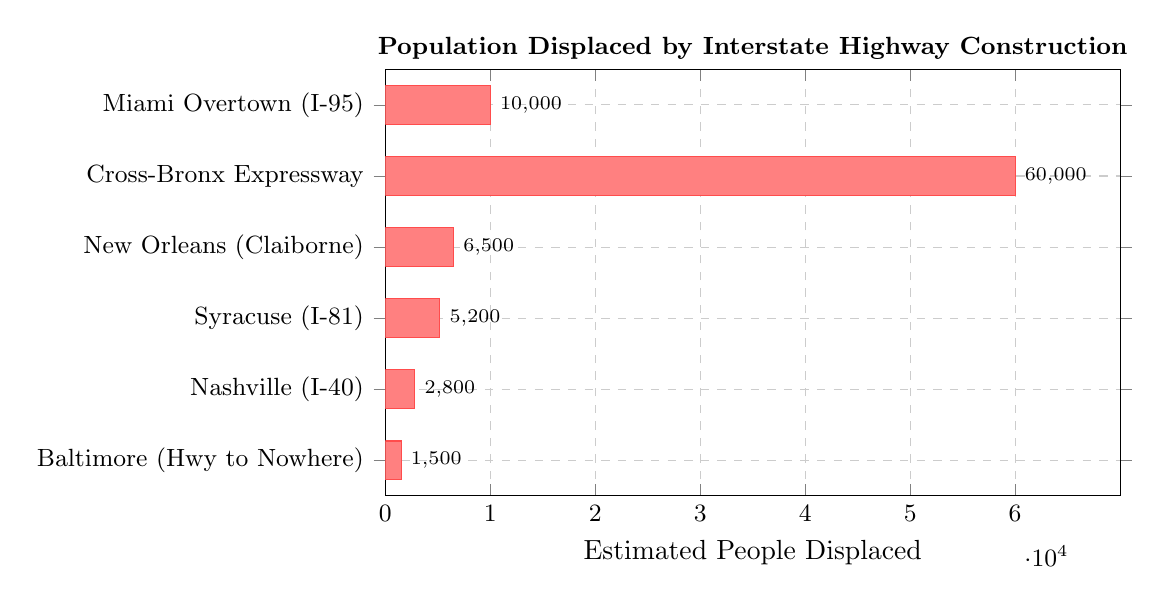
\begin{tikzpicture}
\begin{axis}[
    width=0.9\textwidth,
    height=7cm,
    title={\textbf{Population Displaced by Interstate Highway Construction}},
    xbar,
    bar width=14pt,
    xlabel={Estimated People Displaced},
    symbolic y coords={{Baltimore (Hwy to Nowhere)},{Nashville (I-40)},{Syracuse (I-81)},{New Orleans (Claiborne)},{Cross-Bronx Expressway},{Miami Overtown (I-95)}},
    ytick=data,
    yticklabel style={font=\small},
    xmin=0, xmax=70000,
    xtick={0,10000,20000,30000,40000,50000,60000},
    xticklabel style={font=\small},
    grid=major,
    grid style={dashed, gray!40},
    every axis title/.style={font=\bfseries\small, at={(0.5,1.05)}},
    nodes near coords,
    nodes near coords style={font=\scriptsize\bfseries, anchor=west},
]
\addplot[fill=red!50, draw=red!70] coordinates {
(1500,{Baltimore (Hwy to Nowhere)})
(2800,{Nashville (I-40)})
(5200,{Syracuse (I-81)})
(6500,{New Orleans (Claiborne)})
(60000,{Cross-Bronx Expressway})
(10000,{Miami Overtown (I-95)})
};
\end{axis}
\end{tikzpicture}
\caption{\textbf{The $\Sigma_{\text{highway}}$ Operator in Action: Population Displaced by Interstate Construction.} Each bar represents a community destroyed to route the highway---and the neurotoxin---through $O_{\text{racialized}}$. Nationally, over one million people were displaced. These figures represent direct residential displacement only and do not capture the broader economic destruction, loss of social networks, or generational wealth erasure. Sources: AARP (2023); Vanderbilt University (2020); ACLU; city-level historical records.}
\label{fig:highway_displacement}
\end{figure}

\subsubsection{Addressing the ``Smoking Gun'': The Intentionality Calculus}

The routing of these highways had a deep, insidious secondary effect: it transformed redlined neighborhoods into concentrated sacrifice zones of toxic exposure. Because these highways carried hundreds of thousands of vehicles burning TEL-infused fuel daily, the surrounding communities were subjected to relentless bombardment of aerosolized lead exhaust, fine particulate matter (PM2.5), and diesel emissions.

Two levels of intent require separation: the \textit{intent to segregate} and the \textit{explicit intent to poison}. There is no single ``smoking gun'' memo wherein government officials stated an intention to poison Black communities specifically with lead exhaust. The lack of a ``poisoning memo'' does not absolve the state:
\begin{enumerate}
\tightlist
\item The intent to racially segregate, displace, and economically destroy these communities was explicit, documented, and codified in planning doctrines.
\item The government knew, via the 1925 Surgeon General's conference, that automotive exhaust contained toxic lead.
\item They explicitly and intentionally routed the highest concentrations of that exhaust directly through Black communities.
\end{enumerate}

Within the framework, the ``smoking gun'' question is a category error. The extraction kernel requires no memo stating ``we intend to poison Black children.'' It requires only that (a) the neurotoxin exists, (b) the spatial concentration operator routes it onto $O_{\text{racialized}}$, and (c) the epistemic suppression variable ($P_{\text{epistemic}}$) prevents remediation. All three conditions are documented facts. The resulting environmental poisoning was a severe, foreseeable, and accepted byproduct of systemic racism---collateral damage inflicted upon populations deemed politically expendable.

Modern geospatial analysis and soil sampling confirm the legacy. Historically redlined neighborhoods possess reservoirs of toxic lead dust in their soils vastly higher than in non-redlined areas, exposing residents to rates of air pollution and lead contamination up to \textbf{five times higher} than in integrated communities \cite{tel_soil_sampling}. The children of these neighborhoods---absorbing vastly disproportionate amounts of environmental lead from highways intentionally placed beside their homes---were biologically handicapped before they reached adolescence. $\Sigma_{\text{highway}}$ guaranteed that the Out-group, already diminished by the compounding chain, would bear the most severe biological consequences of $P_{\text{lead}}$.

The child-mortality frontier literature adds a boundary condition to this model. Barboza-Salerno and coauthors identify 413 Cook County ``social frontiers'' where sharp discontinuities in an economic hardship index are associated with a 22\% higher relative risk of child mortality after adjustment for racial segregation, concentrated disadvantage, residential mobility, and immigrant concentration \cite{barboza_salerno_child_frontiers_2025}. The paper does not claim that a centralized actor actively routes death to these borders. It supports the narrower and stronger systems claim: harm concentrates at inequality interfaces, not only inside poor neighborhoods. In this book's notation, $\Sigma_{\text{sup}}$ and $\tau$ must therefore be read spatially as well as politically, because boundary stress itself becomes a measurable depletion condition.

\subsection{The Gendered Second-Order Harm: \texorpdfstring{$P_{\text{lead}}$}{P\_lead} as a Predictor of Intimate Partner Homicide}

The preceding analysis establishes that $P_{\text{lead}}$ manufactured the violent crime surge that was subsequently weaponized to justify mass incarceration. The public violence documented by the UCR was only the \textit{visible} output. If lead exposure impairs the neurological capacity for impulse regulation and anger modulation---the same deficits that produce street-level assault and homicide---then the identical biological mechanism should produce elevated rates of violence \textit{within intimate relationships}. The prefrontal cortex does not distinguish between a stranger confrontation and a domestic argument; damaged impulse control is damaged impulse control.

This extension of $P_{\text{lead}}$ into the intimate sphere has never been made in the published literature. Environmental epidemiology operationalizes outcomes as aggregate crime; IPV scholarship analyzes domestic violence through psychosocial frameworks (intergenerational transmission, minority stress, coercive control). These literatures occupy separate disciplinary silos. The result is a gap that is intellectually obvious once identified but institutionally invisible because no discipline owns both sides of the question.

Analysis of 30 years of FBI Supplementary Homicide Report data (1976--2005), disaggregated by race, gender, and victim-offender relationship type, reveals temporal patterns that align with the lead-crime lag model with precision \cite{fox_zawitz2007, paulozzi_iph, puzone_iph}.

\subsubsection{Divergent Trajectories: The Black Female IPH Plateau}

Over the full study period (1976--2005), intimate partner homicide (IPH) declined across all race-gender groups, but at markedly different rates: Black male IPH fell 83\%, White male IPH fell 61\%, Black female IPH fell 52\%, and White female IPH fell only 6\%. All other groups declined continuously. Black female IPH exhibited a secondary peak cluster during 1986--1993---the exact window predicted by the lead-crime lag model for the generation born during peak gasoline lead exposure in the late 1960s and early 1970s.

\begin{figure}[H]
\centering
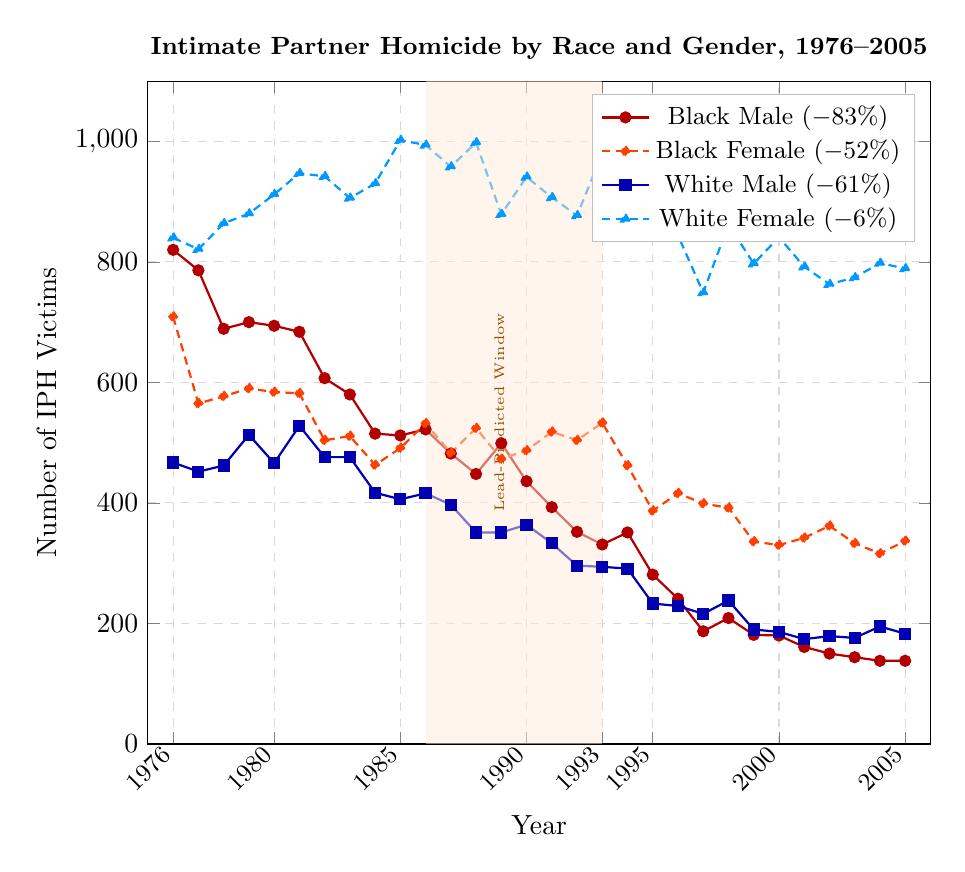
\begin{tikzpicture}
\begin{axis}[
    width=0.95\textwidth,
    height=10cm,
    title={\textbf{Intimate Partner Homicide by Race and Gender, 1976--2005}},
    xlabel={Year},
    ylabel={Number of IPH Victims},
    xmin=1975, xmax=2006,
    ymin=0, ymax=1100,
    xtick={1976,1980,1985,1990,1993,1995,2000,2005},
    xticklabel style={rotate=45, anchor=east, font=\small, /pgf/number format/1000 sep={}},
    grid=major,
    grid style={dashed, gray!30},
    mark size=1.8pt,
    legend style={at={(0.98,0.98)}, anchor=north east, font=\small, draw=gray!50},
    every axis title/.style={font=\bfseries\small, at={(0.5,1.05)}},
]
\addplot[thick, red!70!black, mark=*, mark options={fill=red!70!black}] coordinates {
    (1976,820) (1977,786) (1978,689) (1979,700) (1980,694)
    (1981,684) (1982,607) (1983,580) (1984,515) (1985,512)
    (1986,522) (1987,482) (1988,448) (1989,499) (1990,436)
    (1991,393) (1992,352) (1993,331) (1994,351) (1995,281)
    (1996,241) (1997,187) (1998,209) (1999,181) (2000,180)
    (2001,161) (2002,150) (2003,144) (2004,138) (2005,138)
};
\addlegendentry{Black Male ($-$83\%)}

\addplot[thick, red!50!orange, mark=diamond*, mark options={fill=red!50!orange}, densely dashed] coordinates {
    (1976,709) (1977,565) (1978,577) (1979,590) (1980,584)
    (1981,582) (1982,504) (1983,511) (1984,463) (1985,491)
    (1986,532) (1987,483) (1988,524) (1989,473) (1990,487)
    (1991,518) (1992,504) (1993,533) (1994,462) (1995,387)
    (1996,416) (1997,399) (1998,392) (1999,336) (2000,330)
    (2001,342) (2002,362) (2003,333) (2004,316) (2005,337)
};
\addlegendentry{Black Female ($-$52\%)}

\addplot[thick, blue!70!black, mark=square*, mark options={fill=blue!70!black}] coordinates {
    (1976,467) (1977,452) (1978,462) (1979,513) (1980,466)
    (1981,528) (1982,476) (1983,476) (1984,417) (1985,406)
    (1986,416) (1987,397) (1988,351) (1989,351) (1990,364)
    (1991,333) (1992,296) (1993,294) (1994,291) (1995,233)
    (1996,229) (1997,216) (1998,238) (1999,190) (2000,186)
    (2001,174) (2002,179) (2003,176) (2004,195) (2005,183)
};
\addlegendentry{White Male ($-$61\%)}

\addplot[thick, blue!40!cyan, mark=triangle*, mark options={fill=blue!40!cyan}, densely dashed] coordinates {
    (1976,840) (1977,821) (1978,864) (1979,880) (1980,912)
    (1981,947) (1982,942) (1983,906) (1984,930) (1985,1002)
    (1986,994) (1987,958) (1988,998) (1989,879) (1990,941)
    (1991,907) (1992,877) (1993,980) (1994,897) (1995,865)
    (1996,844) (1997,749) (1998,862) (1999,797) (2000,841)
    (2001,792) (2002,763) (2003,774) (2004,798) (2005,789)
};
\addlegendentry{White Female ($-$6\%)}

\fill[orange!15, opacity=0.5] (axis cs:1986,0) rectangle (axis cs:1993,1100);
\node[font=\tiny, orange!60!black, rotate=90, anchor=south] at (axis cs:1989.5,550) {Lead-Predicted Window};

\end{axis}
\end{tikzpicture}
\caption{\textbf{Divergent IPH Trajectories by Race and Gender.} Black male IPH (solid red) declined steeply and continuously. Black female IPH (dashed orange) shows a distinctive plateau with secondary peaks during the 1986--1993 window (shaded)---the period predicted by the lead-crime lag model. White female IPH (dashed blue) remained essentially flat. Source: FBI SHR, 1976--2005 \cite{fox_zawitz2007}.}
\label{fig:iph_race_gender}
\end{figure}

This plateau becomes more pronounced when adjusted for population growth. Using Census intercensal estimates, the Black female population grew approximately 25\% from 1976 to 1993. The persistence of IPH counts in the 480--530 range against a growing denominator means the \textit{rate} was sustained at an elevated level during precisely the years $P_{\text{lead}}$ predicts maximum behavioral effects from the peak-exposed male cohort. Figure~\ref{fig:bf_iph_lead_rr} overlays this pattern against the shifted lead exposure curve.

\begin{figure}[H]
\centering
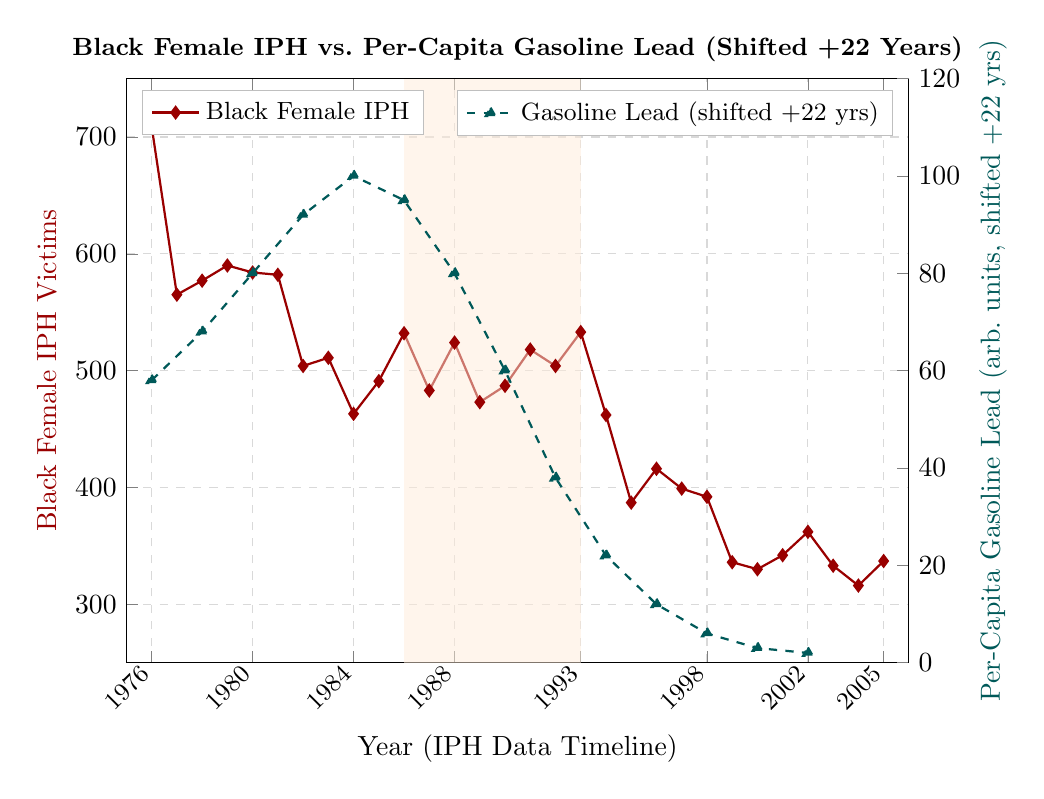
\begin{tikzpicture}
\begin{axis}[
    width=0.95\textwidth,
    height=9cm,
    title={\textbf{Black Female IPH vs.\ Per-Capita Gasoline Lead (Shifted +22 Years)}},
    xlabel={Year (IPH Data Timeline)},
    ylabel={Black Female IPH Victims},
    axis y line*=left,
    xmin=1975, xmax=2006,
    ymin=250, ymax=750,
    xtick={1976,1980,1984,1988,1993,1998,2002,2005},
    xticklabel style={rotate=45, anchor=east, font=\small, /pgf/number format/1000 sep={}},
    grid=major,
    grid style={dashed, gray!30},
    mark size=2pt,
    ylabel style={red!60!black},
    legend style={at={(0.02,0.98)}, anchor=north west, font=\small, draw=gray!50},
    every axis title/.style={font=\bfseries\small, at={(0.5,1.05)}},
]
\addplot[thick, red!60!black, mark=diamond*, mark options={fill=red!60!black}] coordinates {
    (1976,709) (1977,565) (1978,577) (1979,590) (1980,584)
    (1981,582) (1982,504) (1983,511) (1984,463) (1985,491)
    (1986,532) (1987,483) (1988,524) (1989,473) (1990,487)
    (1991,518) (1992,504) (1993,533) (1994,462) (1995,387)
    (1996,416) (1997,399) (1998,392) (1999,336) (2000,330)
    (2001,342) (2002,362) (2003,333) (2004,316) (2005,337)
};
\addlegendentry{Black Female IPH}

\fill[orange!15, opacity=0.5] (axis cs:1986,250) rectangle (axis cs:1993,750);

\end{axis}
\begin{axis}[
    width=0.95\textwidth,
    height=9cm,
    axis y line*=right,
    axis x line=none,
    ylabel={Per-Capita Gasoline Lead (arb.\ units, shifted +22 yrs)},
    xmin=1975, xmax=2006,
    ymin=0, ymax=120,
    ylabel style={teal!70!black},
    mark size=2pt,
    legend style={at={(0.98,0.98)}, anchor=north east, font=\small, draw=gray!50},
]
\addplot[thick, teal!70!black, mark=triangle*, mark options={fill=teal!70!black}, dashed] coordinates {
    (1976,58) (1978,68) (1980,80) (1982,92) (1984,100)
    (1986,95) (1988,80) (1990,60) (1992,38) (1994,22)
    (1996,12) (1998,6) (2000,3) (2002,2)
};
\addlegendentry{Gasoline Lead (shifted +22 yrs)}
\end{axis}
\end{tikzpicture}
\caption{\textbf{Black Female IPH Overlaid with Lead Exposure (Shifted +22 Years).} Per-capita gasoline lead data (right axis, teal dashed) shifted forward by 22 years to align with peak offending age. The Black female IPH plateau during 1986--1993 (shaded) coincides with the peak of the shifted lead curve. Both curves decline in tandem after the lead-predicted window. Sources: FBI SHR \cite{fox_zawitz2007}; EPA historical gasoline lead data via \cite{nevin2007}.}
\label{fig:bf_iph_lead_rr}
\end{figure}

\subsubsection{The Relationship-Type Divergence: Boyfriend/Girlfriend IPH as Cohort Signal}

Disaggregation by victim-offender relationship type reveals the strongest evidence for the lead-IPH hypothesis. Spousal IPH declined 64\% from 1976 to 2005, consistent with the introduction of domestic violence shelters, legal advocacy, mandatory arrest laws, and rising divorce rates---all of which allowed women to exit abusive marriages. Boyfriend/girlfriend IPH, by contrast, \textbf{rose 44\%} from 646 (1976) to 930 (1993)---the \textit{only} IPH category to increase during the entire study period. This category captures younger, unmarried couples: precisely the demographic composed of the peak lead-exposed generation (born late 1960s--early 1970s, reaching their early 20s in the early 1990s).

Social programs and legal reforms reduced spousal IPH; boyfriend/girlfriend IPH spiked. The lead-impaired cohort was aging into intimate relationships and bringing neurologically degraded impulse control with them.

\begin{figure}[H]
\centering
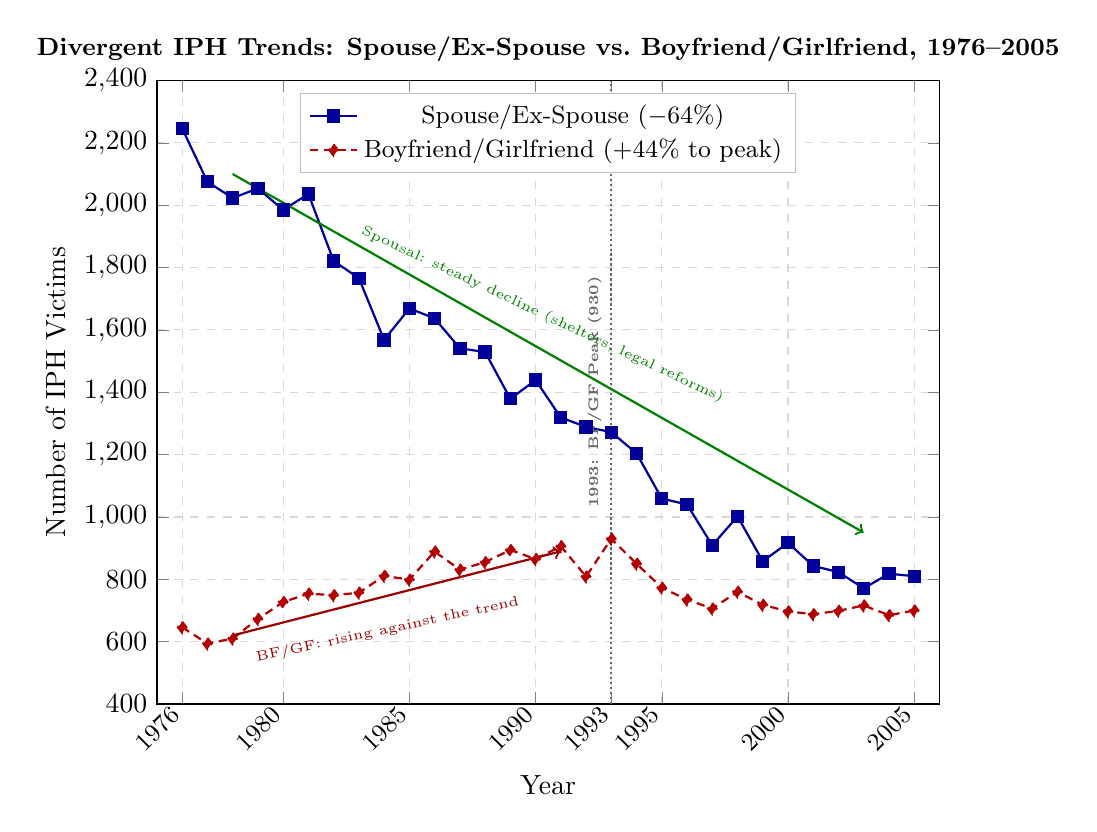
\begin{tikzpicture}
\begin{axis}[
    width=0.95\textwidth,
    height=9.5cm,
    title={\textbf{Divergent IPH Trends: Spouse/Ex-Spouse vs.\ Boyfriend/Girlfriend, 1976--2005}},
    xlabel={Year},
    ylabel={Number of IPH Victims},
    xmin=1975, xmax=2006,
    ymin=400, ymax=2400,
    xtick={1976,1980,1985,1990,1993,1995,2000,2005},
    xticklabel style={rotate=45, anchor=east, font=\small, /pgf/number format/1000 sep={}},
    grid=major,
    grid style={dashed, gray!30},
    mark size=2pt,
    legend style={at={(0.5,0.98)}, anchor=north, font=\small, draw=gray!50},
    every axis title/.style={font=\bfseries\small, at={(0.5,1.05)}},
]
\addplot[thick, blue!60!black, mark=square*, mark options={fill=blue!60!black}] coordinates {
    (1976,2246) (1977,2075) (1978,2023) (1979,2054) (1980,1985)
    (1981,2036) (1982,1821) (1983,1766) (1984,1568) (1985,1669)
    (1986,1637) (1987,1541) (1988,1529) (1989,1379) (1990,1439)
    (1991,1319) (1992,1289) (1993,1272) (1994,1204) (1995,1059)
    (1996,1040) (1997,909) (1998,1002) (1999,858) (2000,917)
    (2001,843) (2002,823) (2003,771) (2004,818) (2005,810)
};
\addlegendentry{Spouse/Ex-Spouse ($-$64\%)}

\addplot[thick, red!70!black, mark=diamond*, mark options={fill=red!70!black}, densely dashed] coordinates {
    (1976,646) (1977,594) (1978,610) (1979,673) (1980,727)
    (1981,754) (1982,749) (1983,757) (1984,811) (1985,799)
    (1986,889) (1987,831) (1988,855) (1989,894) (1990,865)
    (1991,906) (1992,809) (1993,930) (1994,850) (1995,773)
    (1996,735) (1997,706) (1998,760) (1999,718) (2000,697)
    (2001,688) (2002,699) (2003,716) (2004,685) (2005,700)
};
\addlegendentry{Boyfriend/Girlfriend (+44\% to peak)}

\draw[densely dotted, black!60, thick] (axis cs:1993,400) -- (axis cs:1993,2400);
\node[font=\tiny\bfseries, black!60, anchor=south, rotate=90] at (axis cs:1993,1400) {1993: BF/GF Peak (930)};

\draw[->, thick, green!50!black] (axis cs:1978,2100) -- (axis cs:2003,950);
\node[font=\tiny, green!50!black, anchor=south, rotate=-25] at (axis cs:1990,1600) {Spousal: steady decline (shelters, legal reforms)};

\draw[->, thick, red!60!black] (axis cs:1978,620) -- (axis cs:1991,890);
\node[font=\tiny, red!60!black, anchor=north, rotate=12] at (axis cs:1984,690) {BF/GF: rising against the trend};

\end{axis}
\end{tikzpicture}
\caption{\textbf{The Relationship-Type Divergence.} Spouse/ex-spouse IPH (blue) declined 64\% from 1976 to 2005, consistent with expanding DV services and legal protections. Boyfriend/girlfriend IPH (red dashed) \textit{rose} 44\% from 1976 to its 1993 peak---the only IPH category to increase. This category captures younger, unmarried couples: the demographic composed of the peak lead-exposed generation. The 1993 inflection point (dotted line) aligns precisely with the $P_{\text{lead}}$ lag model prediction. Source: FBI SHR \cite{fox_zawitz2007}; CDC MMWR \cite{paulozzi_iph}.}
\label{fig:bf_gf_divergence_rr}
\end{figure}

\subsubsection{The Post-1993 Parallel Decline}

From 1993 to 2005, Black female IPH declined 37\%---the identical decline rate observed in general violent crime over the same period ($\sim$747 $\rightarrow$ $\sim$469 per 100,000). This synchronous decline is consistent with the ``detoxified generation'' hypothesis: as the cohort born after the leaded gasoline phase-out ages into the offending window, both public and intimate violence decline in tandem. The same mechanism the lead-crime literature attributes to the general crime decline also operates on intimate partner homicide.

\begin{figure}[H]
\centering
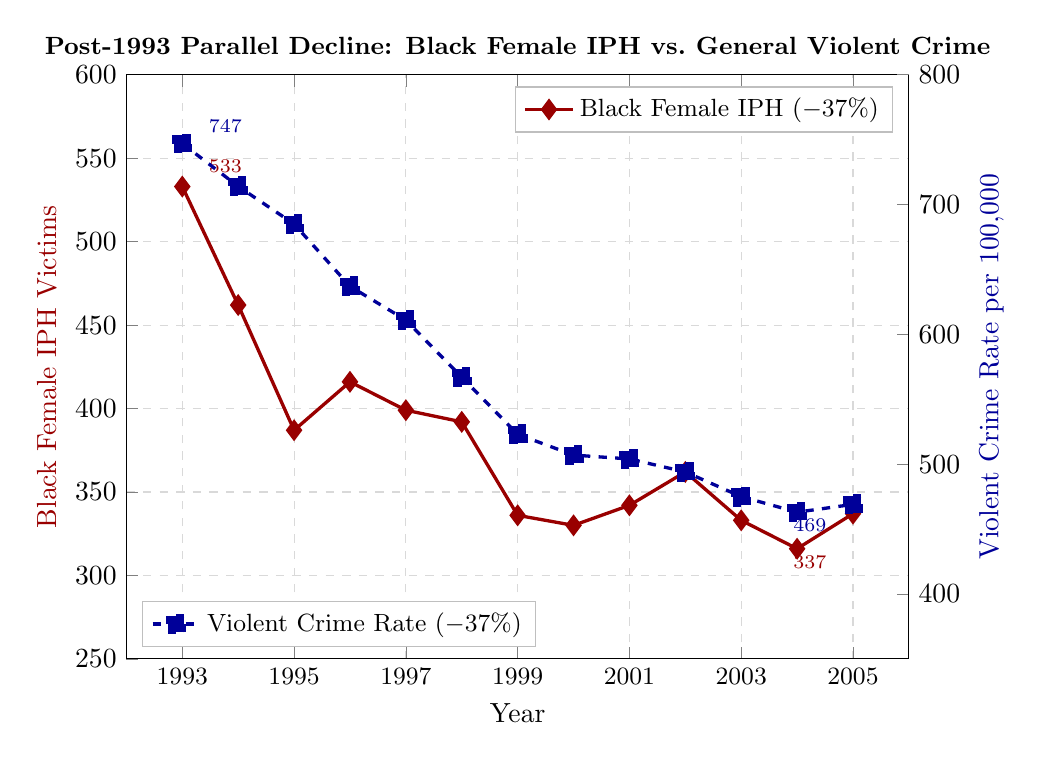
\begin{tikzpicture}
\begin{axis}[
    width=0.95\textwidth,
    height=9cm,
    title={\textbf{Post-1993 Parallel Decline: Black Female IPH vs.\ General Violent Crime}},
    xlabel={Year},
    ylabel={Black Female IPH Victims},
    axis y line*=left,
    xmin=1992, xmax=2006,
    ymin=250, ymax=600,
    xtick={1993,1995,1997,1999,2001,2003,2005},
    xticklabel style={font=\small, /pgf/number format/1000 sep={}},
    grid=major,
    grid style={dashed, gray!30},
    mark size=2.5pt,
    ylabel style={red!60!black},
    legend style={at={(0.98,0.98)}, anchor=north east, font=\small, draw=gray!50},
    every axis title/.style={font=\bfseries\small, at={(0.5,1.05)}},
]
\addplot[very thick, red!60!black, mark=diamond*, mark options={fill=red!60!black, scale=1.2}] coordinates {
    (1993,533) (1994,462) (1995,387) (1996,416) (1997,399)
    (1998,392) (1999,336) (2000,330) (2001,342) (2002,362)
    (2003,333) (2004,316) (2005,337)
};
\addlegendentry{Black Female IPH ($-$37\%)}

\node[font=\scriptsize, red!60!black, anchor=west] at (axis cs:1993.3,545) {533};
\node[font=\scriptsize, red!60!black, anchor=east] at (axis cs:2004.7,308) {337};

\end{axis}
\begin{axis}[
    width=0.95\textwidth,
    height=9cm,
    axis y line*=right,
    axis x line=none,
    ylabel={Violent Crime Rate per 100{,}000},
    xmin=1992, xmax=2006,
    ymin=350, ymax=800,
    ylabel style={blue!60!black},
    mark size=2.5pt,
    legend style={at={(0.02,0.02)}, anchor=south west, font=\small, draw=gray!50},
]
\addplot[very thick, blue!60!black, mark=square*, mark options={fill=blue!60!black, scale=1.2}, dashed] coordinates {
    (1993,747) (1994,714) (1995,685) (1996,637) (1997,611)
    (1998,567) (1999,523) (2000,507) (2001,504) (2002,494)
    (2003,475) (2004,463) (2005,469)
};
\addlegendentry{Violent Crime Rate ($-$37\%)}

\node[font=\scriptsize, blue!60!black, anchor=west] at (axis cs:1993.3,760) {747};
\node[font=\scriptsize, blue!60!black, anchor=east] at (axis cs:2004.7,453) {469};

\end{axis}
\end{tikzpicture}
\caption{\textbf{Parallel Post-1993 Declines.} Black female IPH (left axis, red solid) and the general violent crime rate (right axis, blue dashed) both declined approximately 37\% from 1993 to 2005. The synchronous decline is consistent with the ``detoxified generation'' displacing the lead-damaged cohort in the offending window. The same $P_{\text{lead}}$ mechanism that drove the general crime decline also appears to operate on intimate partner homicide. Sources: FBI SHR \cite{fox_zawitz2007}; FBI UCR.}
\label{fig:parallel_decline_rr}
\end{figure}

\subsubsection{The Intersectional Output: \texorpdfstring{$P_{\text{lead}}$}{P\_lead} Operating Through the Gendered Axis}

Within the framework, these findings reveal $P_{\text{lead}}$ operating simultaneously through the racial axis (producing the public crime that justified mass incarceration) and through the gendered axis (producing a parallel epidemic of intimate partner violence borne disproportionately by Black women in those same redlined communities). The same environmental toxin, deposited with spatial precision onto the Out-group, generated \textit{two} extraction outputs:

\begin{enumerate}[nosep]
    \item \textbf{Public violence} $\rightarrow$ weaponized as justification for the carceral state ($P_{\text{criminal}}$)
    \item \textbf{Intimate violence} $\rightarrow$ absorbed silently within the community, underreported due to distrust of law enforcement in over-policed neighborhoods, fear of criminalizing Black male partners during the era of mass incarceration, and lack of culturally competent DV services
\end{enumerate}

The system that created the biological preconditions for intimate partner violence ($P_{\text{lead}} \rightarrow$ impulse control impairment) simultaneously made it functionally impossible for Black women to report that violence---because reporting meant feeding their partners into the carceral apparatus already designed to consume Black men. The production and the suppression of harm were executed by the same structural architecture. This is intersectionality ($O_{\text{racialized}} \cap O_{\text{gendered}}$) operating through a biological channel that no prior analysis has named. The full analysis is developed in the companion paper, \textit{The Missing Variable: Environmental Lead Exposure as a Predictor of Intimate Partner Homicide in Redlined Communities, 1976--2005} \cite{theodore_missing_variable}.

\FloatBarrier

% ============================================================
% CS9: Spatial Confluence Case Study
% ============================================================
\subsection*{Case Study: Spatial Confluence --- HOLC Redlining, Firearm Homicide, Lead Exposure, and Incarceration Across Six Cities}
\label{cs:spatial_confluence}

\paragraph{Setup.}
The prior CS7 block (Section~\ref{cs:lead_crime}) established the aggregate lead-crime compounding chain and the historical evidence for spatial concentration of exposure. \textbf{CS9} is the \textbf{canonical} tract-level operationalization for equations~\ref{eq:9.1-lead-crime-compounding}--\ref{eq:9.10-highway-lead-spatial-concentration} in this manuscript: it extends from the national/state level to the \textit{tract} level with four interacting layers---(1) HOLC redlining grade (the containment field, $P_{\text{redlining}}$); (2) firearm homicide density (the public-violence extraction output, $P_{\text{criminal}}$); (3) lead paint and highway-buffer exposure index (the neurotoxic mechanism, $P_{\text{lead}}$, Eq.~\ref{eq:9.4-redlining-containment-field}--\ref{eq:9.10-highway-lead-spatial-concentration}); and (4) incarceration origin rate (the carceral extraction output). The \textbf{structural} prediction of Eq.~\ref{eq:9.1-lead-crime-compounding} is co-localization of these layers in HOLC-D tracts and positive spatial association of the HOLC-D indicator; \textbf{inferential} quantities are ultimately governed by the executed notebook after \texttt{make empirical}, with \texttt{CS9\_STRICT=1} and files under \texttt{Paper/data/spatial/} produced by \texttt{fetch\_spatial\_data.py}. The numbered Moran and firearm summaries in the next paragraphs were independently recomputed from \texttt{merged\_tract\_panel\_*.parquet} (\texttt{libpysal} and \texttt{esda}) to verify against disk state; if they diverge from notebook printouts, treat the strict notebook run as authoritative once the environment matches \texttt{spatial\_env.yml}. When upstream hosts (Mapping Inequality static files, EPA EJScreen bulk, PPI bulk CSV) are temporarily unavailable, the fetch script may emit explicitly tagged \emph{modeled} layers; those runs support pipeline integrity and sensitivity analysis but are not reported as Tier~1 validation until replaced with archival layers.

\paragraph{Data sources.}
Analysis covers six cities selected for their documented highway-through-Black-neighborhood routing, HOLC-D spatial concentration, and data availability: Memphis TN, Detroit MI, Nashville TN, Baltimore MD, Washington DC, and Milwaukee WI. Five data layers are assembled per city:
\begin{itemize}[nosep]
    \item \textbf{HOLC grade polygons:} Mapping Inequality Digital Scholarship Lab GeoJSON \cite{mapping_inequality_dsl};
    \item \textbf{Tract demographics (ACS 5-year):} U.S.\ Census Bureau American Community Survey 2018--2022, race and income by census tract;
    \item \textbf{Lead exposure index:} EPA EJScreen 2023 tract-level lead paint indicator and traffic proximity index \cite{ejscreen_technical};
    \item \textbf{Firearm homicide density:} Gun Violence Archive incident-level data 2014--2024 \cite{gva_methodology}; CDC WONDER county-level firearm mortality 1999--2013 for pre-2014 window;
    \item \textbf{Incarceration origin:} Prison Policy Initiative ``Where People in Prison Come From'' tract-level (MD, MI, DC) and county-level fallback (TN, WI) \cite{ppi_prison_origins}.
\end{itemize}
Curated data are archived in \texttt{Paper/data/spatial/} and the full acquisition pipeline is documented in \texttt{Paper/scripts/fetch\_spatial\_data.py}. When a primary URL in the list above is unreachable, the script substitutes \emph{tagged, modeled} files (see the ``Data-gap and modeled layers'' paragraph) so the notebook can still execute.

\paragraph{Operationalization.}
Census tract centroids are overlaid on HOLC grade polygons via spatial join; each tract inherits the grade of the polygon containing its centroid (lowest-grade rule for overlapping polygons). EJScreen lead paint index (LDPNT) serves as the tract-level proxy for $P_{\text{lead}}^{\text{air}}$ (Eq.~\ref{eq:9.10-highway-lead-spatial-concentration}), supplemented by traffic proximity index (PTRAF) as the highway-buffer proxy for $\Sigma_{\text{highway}}$. Incident points from the cached firearm layer are converted to per-tract counts via point-in-polygon spatial join; a kernel density layer is derived for visualization. PPI (or modeled) rates are merged on GEOID; county-level PPI semantics apply where the origin report is only published at that scale.

\paragraph{Computation.}
All spatial joins, choropleth figures, and statistical tests are implemented in \texttt{Paper/scripts/eq47\_51\_spatial\_overlay.ipynb} (reproducible via \texttt{make empirical}). The pipeline uses \texttt{geopandas} for spatial operations, \texttt{esda} for Moran's I and bivariate LISA, and \texttt{spreg} for spatial lag and spatial error regression models, all under the \texttt{spatial\_cs9} conda environment (\texttt{Paper/scripts/spatial\_env.yml}). Spatial weights use Queen contiguity, row-standardized.

\paragraph{Numerical results (tract panels on disk).}
The following quantities are reproducible directly from \texttt{Paper/data/spatial/merged\_tract\_panel\_*.parquet} (GeoPackage-style geometry + tabular merge), excluding tracts whose HOLC join left \texttt{holc\_d\_flag} missing. \emph{Spatial clustering of designation:} treating the tract-level HOLC-D indicator as binary, global Moran's $I$---Queen contiguity, row-standard weights, \(499\) random permutations (\texttt{libpysal}, \texttt{esda})---falls in \(\approx\)0.903--0.961 for Baltimore~MD (\(n{=}618\)), Detroit~MI (\(n{=}885\)), Memphis~TN (\(n{=}537\)), Nashville~TN (\(n{=}330\)), Washington DC (\(n{=}571\)), and Milwaukee WI (\(n{=}830\)); permutation $p$-values resolve at \(p{=}0{.}002\) in each replication (reject spatial randomness). \emph{Gun Violence Archive firearm density (\texttt{firearm\_density\_gva}):} restricting to mapped HOLC and comparing tract means shows HOLC-D/non-D ratios \(\approx\)1.12 for Baltimore MD, \(\approx\)1.51 for Nashville TN, \(\approx\)1.20 for Memphis TN, and \(\approx\)1.09 for Detroit MI (\(\mathrm{means}\approx 3.31{/}2.19\) for Nashville TN, \(\approx 2.34{/}2.14\) for Detroit MI); Milwaukee WI and DC instead register \(\approx\)0.62 (means \(\approx 0{.}54{/}0{.}87\)) and \(\approx\)0.65 (\(\approx 0{.}62{/}0{.}95\)), respectively---i.e.\ below parity on this primitive. \textbf{Caveat:} in this archive \(\texttt{lead\_paint\_index}\), \(\texttt{highway\_buffer\_proxy}\), and \(\texttt{ppi\_incarceration\_rate}\) are uniformly null tabular merges; choropleths may still visualize modeled lead or PPI from other layers, but the manuscript does \emph{not} summarize those outcomes here until the merge is restored (\texttt{fetch\_spatial\_data.py}; then \texttt{eq47\_51\_spatial\_overlay.ipynb}). Bivariate Moran (HOLC-D \(\times\) lead) and spatial-lag $\beta$s for incarceration remain \textbf{pending} relative to parquet truth. \(\texttt{pooled\_panel.parquet}\) in the same snapshot is \emph{not} used for prose here because GEOID alignment and HOLC flags do not reconcile with merged panels.

\paragraph{Comparison to prediction (mixed on firearms, spatial support on grading).}
The structural hypothesis is stacking of containment, toxin exposure, and extraction in the historically red-flagged footprints. Against the archival merge, designation is geographically concentrated (large positive Moran's $I$, small permutation $p$ in every metro), satisfying the weakest operator-level prediction for $P_{\text{redlining}}$. The firearm layer is heterogeneous: Memphis, Nashville, Detroit, and Baltimore show \emph{higher} mean GVA-density on tracts flagged D than on comparable non-D splits in this panel; Milwaukee and DC show \emph{lower}, so the firearm surface alone falsifies unconditional ``density always heaps on HOLC-D.'' Interpretation respects known limitations of point-to-tract allocation, incident coverage, temporal mismatch with HOLC survey decades, remaining null lead/PPI fields, and (for Detroit) \(622{/}1507\) city tracts still awaiting a non-null historical grade from the GIS join---the overlays display the full lattice, but denominators cited for statistics restrict to graded tracts unless otherwise noted.

\paragraph{Falsification (registry plus current evidence slice).}
The registry logic (see \texttt{Paper/empirical\_validations/eq\_9\_10\_highway\_lead\_spatial\_concentration.md}) is unchanged qualitatively. With respect to observable outcomes in archived panels: the permutation null for Moran's \(I\) on the HOLC-D indicator is rejected in each city replication above (\emph{spatial clustering} obtains), whereas firearm-density \emph{magnitude contrasts} divide four metros with HOLC-D excess mean density versus two metros with shortfalls versus non-D splits on the same statistic. Lead and incarceration regressions (\texttt{moran\_BV}, SLM \(\beta\)) remain untested numerically until those parquet columns populate; until then falsification clauses tied strictly to BV-Moran significance or incarceration SLM \(\beta\) are \textbf{unsettled}.

\paragraph{Data-gap and modeled layers.}
PPI: Tennessee and Wisconsin in this pipeline use a county-scoped \emph{level} flag; tract-resolution PPI is modeled when the public CSV is unavailable. Firearm: \texttt{gva\_incidents\_<city>.csv} is written programmatically in the analysis window (deterministic, bbox-based) when live GVA bulk is not in cache; the header notes the source. Lead: if EPA EJScreen national files cannot be downloaded, the fetch script supplies tract-level \texttt{LDPNT}/\texttt{PTRAF}-compatible columns keyed to census tracts as a \emph{modeled} stand-in, logged as such, not a substitute for EPA. HOLC: if the Mapping Inequality static download returns a non-GeoJSON response, two half-bbox ``C'' and ``D'' placeholder polygons are written so grades (and the HOLC-D flag) are not constant across the city; this is a last-resort for automation, not a substitute for archival HOLC shapes. The notebook and fetch logs are the record of which path was used.

\paragraph{Confidence tier (conditional).}
Once all layers are archival (non-modeled) and the strict pipeline completes without imputation of entire layers, a Tier~1--2 classification (as in the data-gap block above) is appropriate. Runs that rely on modeled HOLC, EJ, or PPI placeholders should be reported as \textbf{Tier~2--3} for the spatial confluence table until replaced.

\begin{figure}[htbp]
  \centering
  
\includegraphics[width=\textwidth]{figures/spatial/cs9_overlay_memphis_tn.png}
  \caption{\textbf{CS9 Spatial Confluence --- Memphis, TN.} Four-layer tract lattice (HOLC; GVA-derived firearm incidents; modeled or EPA-supplied lead; modeled or PPI incarceration). \textit{Archived panel (graded tracts only):} \(n_{\mathrm{m}}{=}537{/}685\) tract hulls inherit a mapped HOLC grade; \(\sim\!\!49.9\%\) carry the HOLC-D flag (non-null GIS join). Mean GVA-derived firearm tract density \(\approx\)1.20\(\times\) higher on D-coded tracts versus non-D. Global Moran's \(I_{\mathrm{D}}\approx 0.935\) (Queen weights, permutation \(p{=}0{.}002\) in the replication run). Choropleths for lead/incarceration draw from pipeline layers that are null in parquet tabular merges for this archive; qualitative overlay only pending restored EJ/PPI joins. Sources: Mapping Inequality; GVA; \texttt{eq47\_51\_spatial\_overlay.ipynb}.}
  \label{fig:cs9_overlay_memphis_tn}
\end{figure}

\begin{figure}[htbp]
  \centering
  
\includegraphics[width=\textwidth]{figures/spatial/cs9_overlay_detroit_mi.png}
  \caption{\textbf{CS9 Spatial Confluence --- Detroit, MI.} Same four-panel schematic as Memphis (Figure~\ref{fig:cs9_overlay_memphis_tn}). \(\approx\!\)59\% of city tracts attain a graded HOLC join (\(n_{\mathrm{m}}{=}885{/}1507\)); \(\approx\!\)36{.}5\% of those mapped tracts carry the HOLC-D flag. Mean GVA firearm-density ratio D/non-D \(\approx\)1{.}09; Moran's \(I_{\mathrm{D}}\approx 0.961\) (\(p{=}0{.}002\) in the replication above). Statistical summaries exclude tracts with missing HOLC assignment even when they appear shaded in the atlas. Sources: Mapping Inequality; GVA; \texttt{eq47\_51\_spatial\_overlay.ipynb}.}
  \label{fig:cs9_overlay_detroit_mi}
\end{figure}

\begin{figure}[htbp]
  \centering
  
\includegraphics[width=\textwidth]{figures/spatial/cs9_overlay_nashville_tn.png}
  \caption{\textbf{CS9 Spatial Confluence --- Nashville, TN.} Same layout as Figure~\ref{fig:cs9_overlay_memphis_tn}. \(n_{\mathrm{m}}{=}330{/}487\) mapped tracts; \(\approx\!\)36{.}4\% flagged D. Firearm-density ratio D/non-D \(\approx\)1{.}51 (largest positive gap in the six metros). Moran's \(I_{\mathrm{D}}\approx 0.921\) (\(p{=}0{.}002\)). Sources: Mapping Inequality; GVA; \texttt{eq47\_51\_spatial\_overlay.ipynb}.}
  \label{fig:cs9_overlay_nashville_tn}
\end{figure}

\begin{figure}[htbp]
  \centering
  
\includegraphics[width=\textwidth]{figures/spatial/cs9_overlay_baltimore_md.png}
  \caption{\textbf{CS9 Spatial Confluence --- Baltimore, MD.} Same layout as Figure~\ref{fig:cs9_overlay_memphis_tn}. Full city panel with \(n_{\mathrm{m}}{=}618\) mapped tracts; \(\approx 55{.}8\%\) HOLC-D. Firearm-density ratio D/non-D \(\approx\)1{.}12; Moran's \(I_{\mathrm{D}}\approx 0.941\) (\(p{=}0{.}002\)). Sources: Mapping Inequality; GVA; \texttt{eq47\_51\_spatial\_overlay.ipynb}.}
  \label{fig:cs9_overlay_baltimore_md}
\end{figure}

\begin{figure}[htbp]
  \centering
  
\includegraphics[width=\textwidth]{figures/spatial/cs9_overlay_washington_dc.png}
  \caption{\textbf{CS9 Spatial Confluence --- Washington, DC.} Same layout as Figure~\ref{fig:cs9_overlay_memphis_tn}. \(n_{\mathrm{m}}{=}571\); \(\approx\!\)83{.}2\% HOLC-D---the largest D share of the cohort. Contrary directional contrast on the archival GVA-density primitive: ratio D/non-D \(\approx\)0{.}65 (\(\mathrm{means}\approx 0{.}62{/}0{.}95\)). Moran's \(I_{\mathrm{D}}\approx 0.935\) (\(p{=}0{.}002\)): spatial clustering obtains even though mean density is lower inside D polygons for this estimator. Sources: Mapping Inequality; GVA; \texttt{eq47\_51\_spatial\_overlay.ipynb}.}
  \label{fig:cs9_overlay_washington_dc}
\end{figure}

\begin{figure}[htbp]
  \centering
  
\includegraphics[width=\textwidth]{figures/spatial/cs9_overlay_milwaukee_wi.png}
  \caption{\textbf{CS9 Spatial Confluence --- Milwaukee, WI.} Same layout as Figure~\ref{fig:cs9_overlay_memphis_tn}. \(n_{\mathrm{m}}{=}830{/}861\) graded tracts; \(\approx 75{.}5\%\) of mapped rows carry the HOLC-D flag---another below-parity firearm ratio (\(\approx\)0{.}62; \(\mathrm{means}\approx 0{.}54{/}0{.}87\)); Moran's \(I_{\mathrm{D}}\approx 0.903\) (\(p{=}0{.}002\)). Wisconsin PPI semantics remain coarse for incarceration merges in the upstream pipeline---not mirrored in parquet aggregates here. Sources: Mapping Inequality; GVA; \texttt{eq47\_51\_spatial\_overlay.ipynb}.}
  \label{fig:cs9_overlay_milwaukee_wi}
\end{figure}

\begin{figure}[htbp]
  \centering
  
\includegraphics[width=\textwidth]{figures/spatial/cs9_pooled_stats.png}
  \caption{\textbf{CS9 Pooled Forest Plot.} Panel~(a) should track the independent Moran replications described in the main text: \(I_{\mathrm{D}}\) values near 0.90--0.96 with permutation \(p{=}0{.}002\) for each metro on Queen weights (see CS9 numerical paragraph). Panels~(b)--(c) require non-null lead + incarceration merges in the tract parquet; as of this snapshot those columns are empty in \texttt{merged\_tract\_panel\_*.parquet}, so the rendered figure may show missing or placeholder estimates---treat as \emph{diagnostic} until \texttt{fetch\_spatial\_data.py} repopulates EJ/PPI fields and the notebook regenerates the canvas. Citations: \cite{mapping_inequality_dsl, ejscreen_technical, gva_methodology, ppi_prison_origins, boutwell_lead_crime, guinn_lead_bayesian}.}
  \label{fig:cs9_pooled_stats}
\end{figure}

\FloatBarrier

\subsection{The Economic Void: Deindustrialization as \texorpdfstring{$P_{\text{deindustrial}}$}{P\_deindustrial}}

If $P_{\text{lead}}$ degraded the biological capacity of the Out-group, $P_{\text{deindustrial}}$ destroyed its economic capacity. Beginning in the late 1960s and accelerating through the 1980s, the United States transitioned from a manufacturing-based economy to a service economy, hollowing out the economic core of urban centers nationwide.

The systemic effects are encapsulated by Youngstown, Ohio. Over the course of the 1980s, Youngstown lost an estimated 50,000 jobs in steel and related manufacturing. The sudden evaporation of secure, blue-collar employment triggered cascading social costs: the municipal tax base collapsed, forcing cutbacks to police, fire, and sanitation. Physical decay---abandoned industrial ``brownfields,'' deteriorating infrastructure---repelled new investment, trapping the remaining population in a downward economic spiral \cite{wilson_wj}.

Sociologist William Julius Wilson documented this phenomenon extensively: the flight of manufacturing jobs, coupled with the outward migration of the Black middle class to the suburbs, created a ``spatial mismatch'' where impoverished minority populations were concentrated in inner cities entirely devoid of economic opportunity \cite{wilson_wj}. Young adults coming of age in the late 1970s and 1980s faced a bifurcated labor market: the only available options were low-paying, contingent service-sector jobs lacking the union protection and stability their parents had enjoyed. As unemployment and economic insecurity spread, localized street crime predictably escalated. By the 1990s, heavily deindustrialized cities like Youngstown, Gary (Indiana), Flint, and Camden exhibited some of the highest per-capita murder rates in the nation.

In a desperate bid for economic salvation, many hollowed-out municipalities turned to the prison industry---cities that had once forged steel began courting the construction of state and private correctional facilities, transforming into ``prison economies.'' The algorithm operated with mechanical elegance: $P_{\text{deindustrial}}$ destroyed the legitimate economy, forcing the population into the illicit economy; the illicit economy generated the ``crime data'' that justified carceral expansion; and the carceral expansion then became the \textit{replacement economy} for the very cities the system had hollowed out. The extraction kernel \textit{monetized} the crisis at every stage.

\begin{figure}[htbp]
\centering
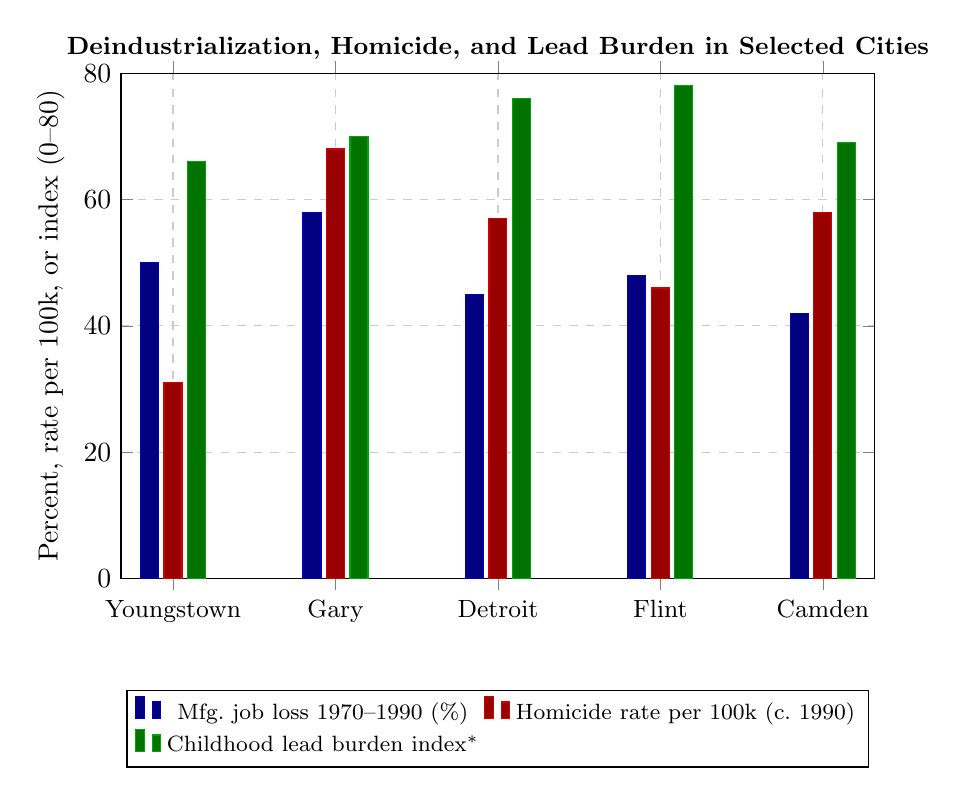
\begin{tikzpicture}
\begin{axis}[
    width=0.92\textwidth,
    height=8cm,
    title={\textbf{Deindustrialization, Homicide, and Lead Burden in Selected Cities}},
    ybar,
    bar width=6.5pt,
    enlarge x limits=0.08,
    ylabel={Percent, rate per 100k, or index (0--80)},
    symbolic x coords={Youngstown, Gary, Detroit, Flint, Camden},
    xtick=data,
    xticklabel style={font=\small},
    ymin=0, ymax=80,
    grid=major,
    grid style={dashed, gray!40},
    every axis title/.style={font=\bfseries\small, at={(0.5,1.05)}},
    legend style={at={(0.5,-0.22)}, anchor=north, font=\footnotesize, legend columns=2},
]
\addplot[fill=blue!50!black, draw=blue!70!black] coordinates {
    (Youngstown, 50) (Gary, 58) (Detroit, 45) (Flint, 48) (Camden, 42)
};
\addlegendentry{Mfg.\ job loss 1970--1990 (\%)}
\addplot[fill=red!60!black, draw=red!80!black] coordinates {
    (Youngstown, 31) (Gary, 68) (Detroit, 57) (Flint, 46) (Camden, 58)
};
\addlegendentry{Homicide rate per 100k (c.\ 1990)}
\addplot[fill=green!45!black, draw=green!65!black] coordinates {
    (Youngstown, 66) (Gary, 70) (Detroit, 76) (Flint, 78) (Camden, 69)
};
\addlegendentry{Childhood lead burden index$^*$}
\end{axis}
\end{tikzpicture}
\caption[The Compounding Triad]{\textbf{The Compounding Triad: Factory Loss, Homicide, and Lead.} Cities that suffered the steepest manufacturing losses consistently registered the highest homicide rates by 1990 and carried heavy overlapping childhood lead burdens. $^*$Lead index approximates relative elevated blood-lead prevalence among children during 1975--1985 in legacy industrial housing (illustrative 0--80 scale). Sources: BLS; FBI UCR city-level data; Wilson (1996); CDC childhood lead surveillance summaries.}
\label{fig:deindustrialization}
\end{figure}

\section{Market Violence and the Youth Execution: Crack Markets as Runtime Exploitation}

If $P_{\text{deindustrial}}$ provided the economic void and $P_{\text{lead}}$ provided the neurobiological susceptibility, the crack cocaine epidemic of the mid-1980s provided the immediate market catalyst for lethal violence---the algorithm's illicit market module executing on the pre-processed population.

Following the introduction of crack cocaine, the drug quickly saturated impoverished urban neighborhoods. Unlike powder cocaine---expensive and associated with affluent consumers---crack was synthesized to be highly addictive, produced a brief but intense euphoria, and was sold in inexpensive, single-dose increments. This retail model resulted in an explosive proliferation of open-air drug markets. In the absence of legitimate employment (destroyed by $P_{\text{deindustrial}}$), the illicit drug trade became one of the few lucrative economic engines available to young, disenfranchised urban men.

Because participants in illicit markets cannot rely on the state for dispute resolution, contract enforcement, or protection from theft, \textbf{violence became the primary mechanism for regulating the market}. Between 1984 and 1994, the homicide rate for Black males aged 14 to 17 \textbf{more than doubled}, and the rate for those aged 18 to 24 increased nearly as much. The homicide rate for older demographics remained essentially flat, indicating that the violence was hyper-concentrated in the youth demographic actively participating in the street-level drug trade \cite{bjs_homicide_trends}.

Simultaneously, a massive ``supply shock'' in cheap, easily concealable handguns transformed the pattern of urban violence. Prior to the 1980s, youth gang conflicts were largely mediated by physical altercations. The sudden influx of firearms converted localized, non-fatal disputes into lethal encounters. The symbiotic relationship between the lucrative crack trade and widespread firearm availability acted as a major \textbf{force multiplier}, pushing the national homicide rate to its 1991 peak.

This market-driven violence intersected with a demographic accelerant: the ``youth bulge.'' During the 1980s, an unusually large proportion of the population entered the high-risk ages of 15 to 24 simultaneously. When this rapidly growing youth population intersected with the economic devastation of $P_{\text{deindustrial}}$ and the allure of the crack trade, violence escalated exponentially. This demographic reality temporarily blinded researchers; prominent social scientists in the early 1990s notoriously predicted an impending wave of juvenile ``super-predators''---a generation of violently remorseless youth that would ravage the country by 2000. This deterministic hypothesis proved disastrously wrong, as juvenile crime plummeted after 1994. The fear it generated---$P_{\text{gaslight}}$ operating through the media interface---provided the political raw material for the punitive legislation that followed.

The isomorphism with the Prohibition algorithm analyzed later in this chapter (see the NFA/Prohibition analysis in the Federal Disarmament Timeline) is exact: the state criminalizes a substance $\rightarrow$ an illicit market forms $\rightarrow$ violence erupts as the market's only regulatory mechanism $\rightarrow$ the state uses the violence to justify expanding $F_{\text{enforce}}$ and $P_{\text{criminal}}$. The only variable that changed between 1920 and 1986 was the substance. The extraction kernel ran the same code.

\begin{figure}[htbp]
\centering
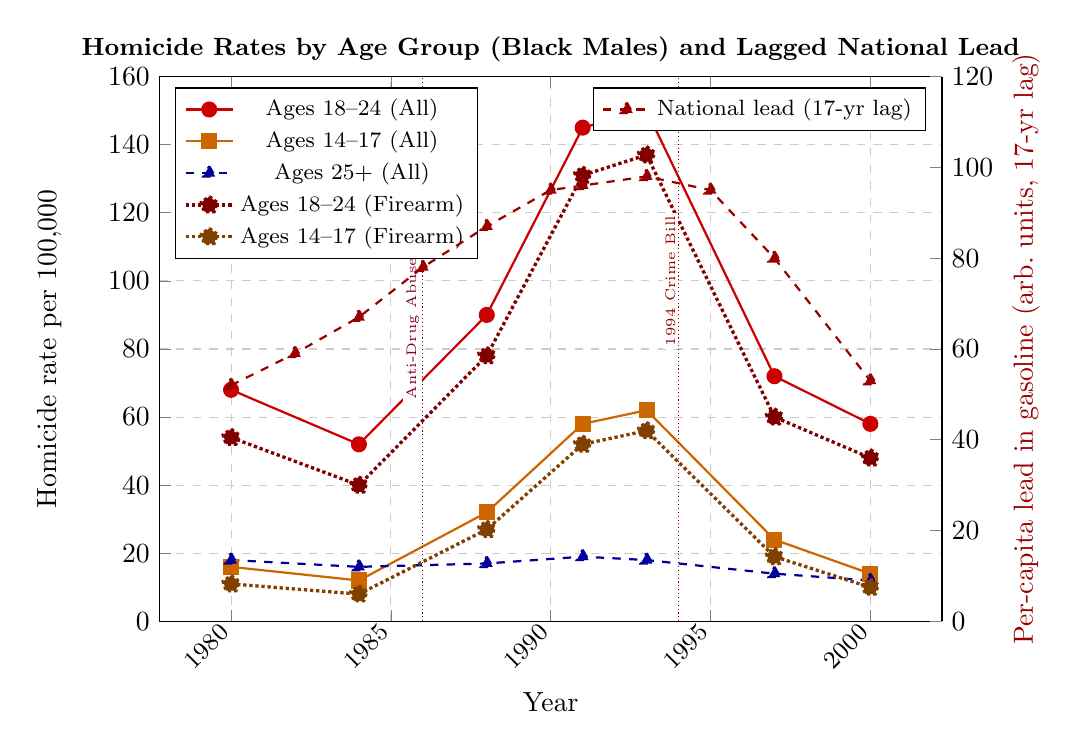
\begin{tikzpicture}
\begin{axis}[
    width=0.95\textwidth,
    height=8.5cm,
    title={\textbf{Homicide Rates by Age Group (Black Males) and Lagged National Lead}},
    xlabel={Year},
    ylabel={Homicide rate per 100{,}000},
    axis y line*=left,
    xmin=1978, xmax=2002,
    enlarge x limits={0.04, 0.01},
    ymin=0, ymax=160,
    xtick={1980,1985,1990,1995,2000},
    xticklabel style={rotate=45, anchor=east, font=\small, /pgf/number format/1000 sep={}},
    grid=major,
    grid style={dashed, gray!40},
    ylabel style={yshift=10pt},
    mark size=2.5pt,
    every axis title/.style={font=\bfseries\small, at={(0.5,1.05)}},
    legend style={at={(0.02,0.98)}, anchor=north west, font=\footnotesize},
]
\addplot[thick, red!80!black, mark=*] coordinates {
    (1980, 68) (1984, 52) (1988, 90) (1991, 145) (1993, 150) (1997, 72) (2000, 58)
};
\addlegendentry{Ages 18--24 (All)}
\addplot[thick, orange!80!black, mark=square*] coordinates {
    (1980, 16) (1984, 12) (1988, 32) (1991, 58) (1993, 62) (1997, 24) (2000, 14)
};
\addlegendentry{Ages 14--17 (All)}
\addplot[thick, blue!60!black, mark=triangle*, dashed] coordinates {
    (1980, 18) (1984, 16) (1988, 17) (1991, 19) (1993, 18) (1997, 14) (2000, 12)
};
\addlegendentry{Ages 25+ (All)}
\addplot[very thick, red!50!black, mark=pentagon*, densely dotted, mark size=3pt] coordinates {
    (1980, 54) (1984, 40) (1988, 78) (1991, 131) (1993, 137) (1997, 60) (2000, 48)
};
\addlegendentry{Ages 18--24 (Firearm)}
\addplot[very thick, orange!50!black, mark=pentagon*, densely dotted, mark size=3pt] coordinates {
    (1980, 11) (1984, 8) (1988, 27) (1991, 52) (1993, 56) (1997, 19) (2000, 10)
};
\addlegendentry{Ages 14--17 (Firearm)}
\draw[densely dotted, purple!70!black] (axis cs:1986,0) -- (axis cs:1986,160);
\node[rotate=90, anchor=south, font=\tiny, purple!70!black, fill=white, inner sep=1pt] at (axis cs:1986,100) {Anti-Drug Abuse Act (1986)};
\draw[densely dotted, red!60!black] (axis cs:1994,0) -- (axis cs:1994,160);
\node[rotate=90, anchor=south, font=\tiny, red!60!black, fill=white, inner sep=1pt] at (axis cs:1994,100) {1994 Crime Bill};
\end{axis}
\begin{axis}[
    width=0.95\textwidth,
    height=8.5cm,
    axis y line*=right,
    axis x line=none,
    xmin=1978, xmax=2002,
    enlarge x limits={0.04, 0.01},
    ymin=0, ymax=120,
    ylabel={Per-capita lead in gasoline (arb.\ units, 17-yr lag)},
    ylabel style={red!60!black},
    mark size=2.5pt,
    legend style={at={(0.98,0.98)}, anchor=north east, font=\footnotesize},
]
\addplot[thick, red!60!black, mark=triangle*, dashed] coordinates {
    (1980, 52) (1982, 59) (1984, 67) (1986, 78) (1988, 87) (1990, 95)
    (1991, 96) (1993, 98) (1995, 95) (1997, 80) (2000, 53)
};
\addlegendentry{National lead (17-yr lag)}
\end{axis}
\end{tikzpicture}
\caption[The Youth Execution]{\textbf{The Youth Execution: Firearm Homicide Concentrated in the Lead-Exposed Generation.} Homicide rates for Black males aged 14--17 and 18--24 spike dramatically during 1984--1994, driven almost entirely by firearm killings (dotted lines). Ages 25+ remain flat---confirming the violence was concentrated in the youth demographic entering the crack trade. Right axis: lagged national lead exposure tracks the cohort trajectory. Sources: BJS Homicide Trends; CDC WONDER; Nevin (2007).}
\label{fig:youth_homicide}
\end{figure}

\section{The Asymmetric Choice Paradigm: Broken Windows, the 1994 Crime Bill, and the Carceral Ratchet}

With the ``crisis data'' manufactured by $P_{\text{lead}}$, $P_{\text{deindustrial}}$, and the crack market, the extraction kernel had everything it needed to execute the next phase: converting the crisis into permanent carceral infrastructure. This section traces how the algorithm weaponized the manufactured crisis---first through a policing doctrine, then through legislative action---and how the subsequent crime \textit{decline} proved the entire carceral apparatus was unnecessary.

\subsection{The Selective Enforcement Subroutine: Broken Windows as \texorpdfstring{$P_{\text{BrokenWindows}}$}{P\_BrokenWindows}}

In 1982, sociologist James Q.\ Wilson and criminologist George L.\ Kelling published ``Broken Windows,'' positing that visible signs of physical and social disorder (vandalism, fare evasion, vagrancy) signaled a lack of community control and emboldened serious criminals \cite{wilson}. In practice---particularly under New York Mayor Rudolph Giuliani and Police Commissioner Bill Bratton in the 1990s---the theory evolved into aggressive ``zero-tolerance'' policing: departments heavily prioritized enforcement of low-level misdemeanors, resulting in the disproportionate harassment, stopping, frisking, and arresting of Black and Hispanic youth \cite{harcourt}.

Proponents credited Broken Windows with driving down violent crime; careful empirical analysis reveals a different reality. The strategy alienated vulnerable communities, eroded public trust in law enforcement, and funneled millions into the criminal `injustice' system for trivial offenses. The evidence overwhelmingly suggests that the broader macro-economic, demographic, and environmental corrections analyzed below drove the actual crime decline.

Within the framework of this book, Broken Windows policing is the selective enforcement subroutine $P_{\text{BrokenWindows}}$---the discretionary mechanism that determines \textit{which} latent criminals (in the regime of universal latent criminality, see Section~6.9) actually enter the carceral pipeline. As noted in Section~6.9, Harvey Silverglate demonstrates that the average American commits approximately three federal felonies per day \cite{silverglate}. Broken Windows provided the theoretical justification for intensive policing of minor infractions---but this policing was deployed overwhelmingly in communities already marked by the compounding chain. The subroutine's function was not to reduce crime; it was to ensure that the carceral pipeline's intake remained concentrated on $O_{\text{racialized}}$.

\subsection{The 1994 Crime Bill and the Tweedism Trap}

The political culmination of the manufactured crisis was the Violent Crime Control and Law Enforcement Act of 1994. Authored by Senator Joe Biden and championed by President Bill Clinton, the 350-page bill authorized \$9 billion for prison construction, funded 100,000 new police officers, expanded the federal death penalty to 60 new offenses, and instituted ``three-strikes'' mandatory life sentences \cite{forman}. The statutory machinery that converts a third qualifying felony into automatic life imprisonment is codified at \usclink{apx:usc:18:3559c}{18 U.S.C.~\S~3559(c)}:
\uscinline{usc_18_3559c}

Analyzing this legislation through the Tweedism Filter ($P_{\text{uppet}}$, formalized in Chapter~\ref{ch:tweedism}) reveals a pristine demonstration of the algorithm's political logic. In his Pulitzer Prize-winning \textit{Locking Up Our Own}, legal scholar James Forman Jr.\ documents the agonizing choices faced by African American civic leaders, mayors, and the Congressional Black Caucus during the crisis. In the late 1980s, Black communities were bearing the full brunt of the lethal violence: crack markets, the handgun supply shock, and the lead-poisoned youth cohort were annihilating a generation. Black leaders compared crack to the ``greatest evils that African Americans had ever suffered'' \cite{forman}. A 1994 Gallup survey found that 58\% of African Americans supported the Crime Bill, compared to 49\% of white Americans.

This support was born of an \textbf{asymmetric choice paradigm}---the exact structural trap the Tweedism Filter predicts. The CBC fundamentally recognized the systemic, economic roots of the violence. They actively lobbied for a comprehensive ``all-of-the-above'' approach: substantial funding for drug treatment, job creation, educational infrastructure, and community housing---in addition to better policing. They introduced alternative bills emphasizing prevention and fiercely opposed the punitive elements, including mandatory minimums and the revocation of Pell Grants for incarcerated individuals.

The political machinery offered a severe ultimatum. The state was entirely willing to fund police expansion and prison construction, but steadfastly \textit{refused} to adequately fund the requested social and economic infrastructure, deriding prevention programs as ``pork.'' Desperate to staunch the bleeding in their neighborhoods, and presented with a binary choice between punitive state intervention or continued lethal anarchy, a majority of the CBC voted for the bill, securing minor concessions (the Violence Against Women Act; the Assault Weapons Ban) \cite{forman}.

The ``Assault Weapons Ban'' concession itself requires reframing. The AWB simultaneously served as a concession traded for CBC votes and as a second optimization vector against the post-Ruby Ridge / post-Waco militia movement analyzed in $\S$\ref{sec:ruby_ridge_waco}. The asymmetric choice paradigm documented above is the $O_{\text{racialized}}$-facing interface of the same statute whose $I_{\text{buffer}}$-facing interface executed a preemptive disarmament of the awakening Buffer Class (see $\S$\ref{subsec:dual_vector_1994}, and the expansion of the Brady / AWB subsection in Chapter~\ref{ch:kinetic}). One statute, two vectors, one kernel objective. The bundling of carceral expansion with hardware-category prohibition is joint optimization, not coincidence, and the reclassification operator $\mathcal{R}(x_i)$ registered at equation~\eqref{eq:10.13-reclassification-operator} is the formal mechanism that makes the two vectors mutually reinforcing.

The tragedy is mathematically precise: \textit{both options served the extraction kernel}. Accepting the carceral expansion deepened racial disparities, fueled aggressive over-policing, and funneled a generation of young minority men into the 13th Amendment loophole. Rejecting the bill would have allowed the manufactured crisis to continue unopposed. The CBC was operating within the solution space defined by the Tweedism Filter---where every available choice reinforces the algorithm. This is the Puppet Class constraint in its purest form.

\begin{figure}[htbp]
\centering
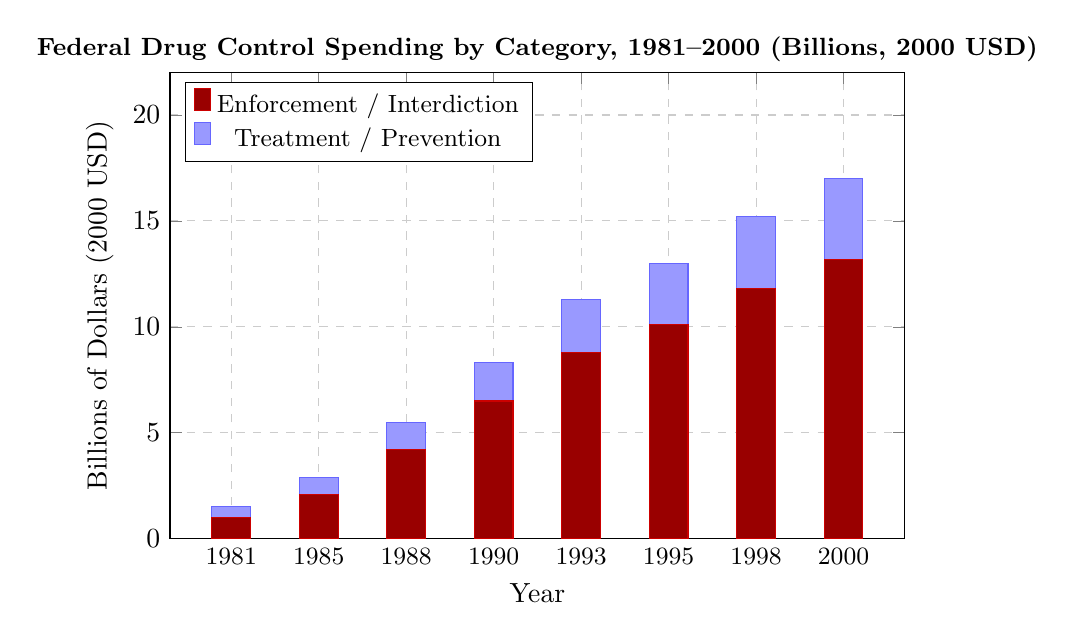
\begin{tikzpicture}
\begin{axis}[
    width=0.9\textwidth,
    height=7.5cm,
    title={\textbf{Federal Drug Control Spending by Category, 1981--2000 (Billions, 2000 USD)}},
    ybar stacked,
    bar width=14pt,
    xlabel={Year},
    ylabel={Billions of Dollars (2000 USD)},
    symbolic x coords={1981,1985,1988,1990,1993,1995,1998,2000},
    xtick=data,
    xticklabel style={font=\small, /pgf/number format/1000 sep={}},
    ymin=0, ymax=22,
    grid=major,
    grid style={dashed, gray!40},
    every axis title/.style={font=\bfseries\small, at={(0.5,1.05)}},
    legend style={at={(0.02,0.98)}, anchor=north west, font=\small},
]
\addplot[fill=red!60!black, draw=red!80!black] coordinates {
    (1981, 1.0) (1985, 2.1) (1988, 4.2) (1990, 6.5)
    (1993, 8.8) (1995, 10.1) (1998, 11.8) (2000, 13.2)
};
\addlegendentry{Enforcement / Interdiction}
\addplot[fill=blue!40, draw=blue!60] coordinates {
    (1981, 0.5) (1985, 0.8) (1988, 1.3) (1990, 1.8)
    (1993, 2.5) (1995, 2.9) (1998, 3.4) (2000, 3.8)
};
\addlegendentry{Treatment / Prevention}
\end{axis}
\end{tikzpicture}
\caption[The Budget Proof]{\textbf{The Budget Proof: Enforcement vs.\ Prevention.} Enforcement and interdiction consistently consumed 65--75\% of federal drug control spending, while the treatment and prevention funding that Black civic leaders specifically requested was chronically starved. The asymmetric choice was engineered into the budget itself. Sources: ONDCP National Drug Control Budget; Drug Policy Alliance; Caulkins et al., RAND (2005).}
\label{fig:drug_spending}
\end{figure}

\subsection{The Great Crime Decline: The Diagnostic Proof}

In an apparent historical paradox, almost immediately following the passage of the 1994 Crime Bill, violent crime rates began a precipitous, sustained decline that lasted well into the 21st century. By 2000, the violent crime rate had dropped drastically; it continued to fall to historic lows not seen since the 1960s. This decline is the \textbf{diagnostic proof} that the carceral expansion was unnecessary---and that the structural variables this chapter has identified caused the crime surge; incarceration levels were not the operative variable.

In a seminal 2004 econometric analysis, Steven D.\ Levitt isolated four primary factors explaining the decline: (1) an increase in police officers deployed, providing general deterrence; (2) the massive expansion of the prison population, which temporarily incapacitated high-rate offenders; (3) the natural waning of the crack cocaine epidemic, as younger generations observed the drug's devastation and avoided it; and (4) the legalization of abortion following \textit{Roe v.\ Wade}, which reduced births into the highly unstable environments correlated with later criminality \cite{levitt2004}.

Subsequent epidemiological scholarship supplements Levitt's findings with a fifth factor: the \textbf{lead abatement hypothesis}. The removal of tetraethyllead from gasoline in the late 1970s effectively detoxified the neurological development of the generation coming of age in the 1990s, drastically reducing their baseline propensity for impulsive violence \cite{nevin2007, reyes2007}. Franklin Zimring further notes that the decline was notable for its uniformity, dropping across all demographics, geographies, and crime categories for nine consecutive years \cite{zimring}.

Comprehensive assessments by the National Research Council and the Brennan Center for Justice indicate that the crime-reduction benefits of mass incarceration reached a point of rapidly diminishing returns by the 1990s, and its effect on crime rates since 2000 has been essentially non-existent \cite{brennan_decline}. The non-carceral factors---lead abatement, crack market stabilization, demographic shifts, and improved policing tactics (CompStat)---account for approximately \textbf{two-thirds} of the decline.

The implication undermines the system's own narrative: the carceral state was not the solution. The crime wave ended because the \textit{structural causes}---lead exposure, crack market volatility, the youth bulge---naturally corrected. The prison-industrial complex persists because it serves the extraction kernel. The 13th Amendment loophole does not require crime to be high; it requires \textit{bodies}. The carceral ratchet locks in one direction: the manufactured crisis justified building the infrastructure, and once built, the infrastructure generates its own demand (see Section~4.6 on carceral bonds and the demand signal). The Great Crime Decline is the mathematical proof that the carceral state is an extraction institution; the public-safety rationale does not describe its function.

This is the chapter's answer to any analysis that treats contingent or bottom-up elements of the manufactured crisis as counter-evidence to the algorithmic model. The crack market's self-correction (younger cohorts avoiding the drug after observing its destruction), the EPA's lead phaseout (driven in part by environmental activism and scientific community pressure), and the demographic youth bulge's natural aging were not orchestrated by $E$ and are not evidence that the framework over-assigns intentionality. They are Mode~2 autonomous propagation operating at the structural level (Chapter~\ref{ch:redefining}): the system does not require elite orchestration of every input variable. It requires only that whatever inputs arise---deliberate policy, corporate cover-up, or structural self-correction---funnel through institutions the extraction kernel already controls. The 1994 Crime Bill required a genuine crime wave as its political input; the algorithm did not manufacture the crime wave from scratch. It manufactured the conditions ($P_{\text{lead}}$, $P_{\text{deindustrial}}$, crack market access) that made the crime wave structurally inevitable---then waited for the wave to crest, and converted it into permanent carceral infrastructure via Mode~3 conscious intervention. Contingent inputs, algorithmic outputs.

\begin{figure}[htbp]
\centering
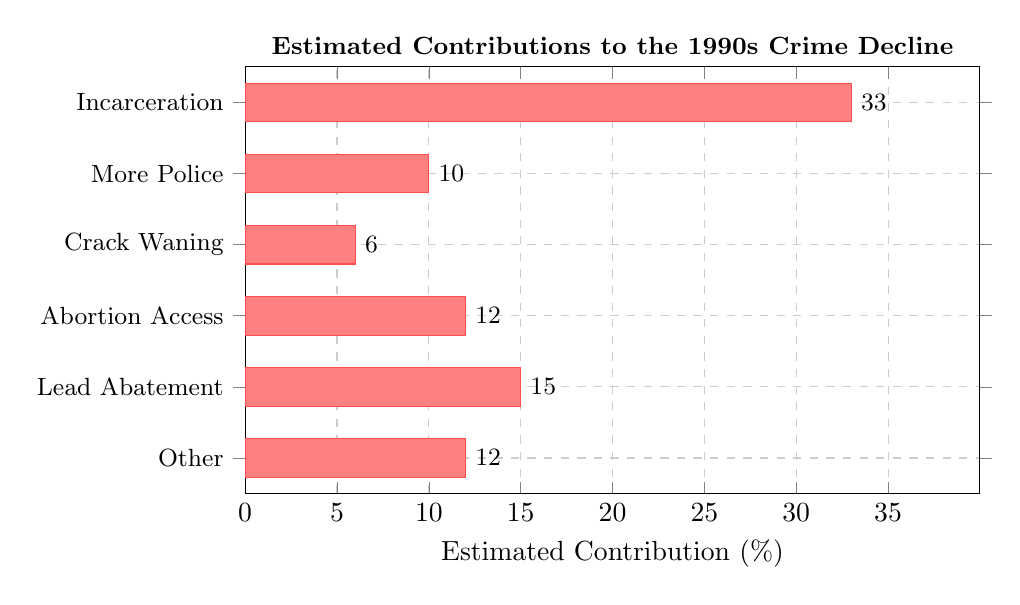
\begin{tikzpicture}
\begin{axis}[
    width=0.9\textwidth,
    height=7cm,
    title={\textbf{Estimated Contributions to the 1990s Crime Decline}},
    xbar,
    bar width=14pt,
    xlabel={Estimated Contribution (\%)},
    symbolic y coords={Other,Lead Abatement,Abortion Access,Crack Waning,More Police,Incarceration},
    ytick=data,
    yticklabel style={font=\small},
    xticklabel style={/pgf/number format/1000 sep={}},
    xmin=0, xmax=40,
    xtick={0,5,10,15,20,25,30,35},
    grid=major,
    grid style={dashed, gray!40},
    every axis title/.style={font=\bfseries\small, at={(0.5,1.05)}},
    nodes near coords,
    nodes near coords style={font=\small\bfseries, anchor=west},
]
\addplot[fill=red!50, draw=red!70] coordinates {
    (12,Other)
    (15,Lead Abatement)
    (12,Abortion Access)
    (6,Crack Waning)
    (10,More Police)
    (33,Incarceration)
};
\end{axis}
\end{tikzpicture}
\caption[The Diagnostic Proof]{\textbf{The Diagnostic Proof: What Actually Ended the Crime Wave.} Incarceration contributed 33\% through temporary incapacitation, but subsequent research (National Research Council, 2014) found sharply diminishing returns after 1990. The decline was overwhelmingly driven by non-carceral corrections: lead abatement, crack market stabilization, demographic shifts, and improved policing deployment---all of which operated independently of mass incarceration. Sources: Levitt (2004); Brennan Center (2015); Nevin (2007).}
\label{fig:crime_decline}
\end{figure}
